\documentclass {ctuthesis}
\usepackage{dirtytalk}
% \usepackage{listings}
\usepackage{float}
\usepackage{graphicx}
% \usepackage{glossaries}
\graphicspath{ {./img/} }

% \usepackage[table,xcdraw]{xcolor}
\usepackage{tabularx}

\usepackage{rotating}

\usepackage{nomencl}
\providecommand{\printnomenclature}{\printglossary}
\providecommand{\makenomenclature}{\makeglossary}
\renewcommand{\nomname}{Slovník}
\settowidth{\nomlabelwidth}{AAAAAAAA}
\makenomenclature

\usepackage{afterpage}

\newcommand\blankpage{
    \null
    \thispagestyle{empty}
    \addtocounter{page}{-1}
    \newpage
    }


\ctusetup{
    pkg-listings = true,
	doctype-czech = {Bakalářská práce},
	xfaculty = F3,
	mainlanguage = czech,
	titlelanguage = czech,
	title-english = {Competency-based employee search},
	title-czech = {Vyhledávání zaměstnanců dle kompetence},
	department-czech = {Katedra počítačů},
	author = {DOMINIK KOUBA},
	supervisor = {Ing. Lukáš Zoubek},
	supervisor-address = {Katedra ekonomiky, manažerství a humanitních věd},
	fieldofstudy-czech = {Softwarové inženýrství a technologie},
% 	subfieldofstudy-czech = {žádné},
	keywords-czech = {kompetence, vyhledávání, osoba, pracoviště, znalost, FEL, ČVUT, ontologie, SKOS}, %TODO
	keywords-english = {competence, search, people, workplace, knowledge, FEE, CTU, ontology, SKOS}, %TODO
	front-specification = true,
	specification-file = {zadani.pdf}, % PDF s tvym zadanim prace
	day = 21,
	month = 5,
	year = 2019,
}



% ===========================

% 
\nomenclature{FEL ČVUT}{Fakulta elektrotechnická Českého vysokého učení technického v Praze}
\nomenclature{FIT ČVUT}{Fakulta informačních technologií Českého vysokého učení technického v Praze}
\nomenclature{FOL}{Logika prvního řádu (angl. First order logic)}
\nomenclature{CRUD}{Operace vytvoření, čtení, změna a vymazaní (angl. create, read, update a delete)}
\nomenclature{SKOS}{Systém pro organizaci znalostí (angl. Simple Knowledge Organization System)}
\nomenclature{OWL}{Webový ontologický jazyk (angl. Web Ontology Language)}
\nomenclature{SPARQL}{Protokol a RDF dotazovací jazyk (angl. Protocol and RDF Query Language)}
\nomenclature{RDF}{Framework pro popis zdrojů (angl. Resource Description Framework)}
\nomenclature{XML}{Rozšiřitelný značkovací jazyk (angl. Extensible Markup Language)}
\nomenclature{UFO}{Unifikovaná základní ontologie (angl. Unified Foundational Ontology)}
\nomenclature{URI}{Uniformní identifikátor zdroje (angl. Uniform Resource Identifier)}
\nomenclature{JSON-LD}{Javascriptová objektová notace pro propojená data (angl. JavaScript Object Notation for Linked Data)}
\nomenclature{UML}{Unifikovaný modelovací jazyk (angl. Unified Modelling Language)}
\nomenclature{API}{Rozhraní pro programování aplikací (angl. Application Programming Interface), v našem kontextu spíše webová služba nebo rozhraní pro poskytování dat}
\nomenclature{SPI}{Rozhraní poskytovatele služby (angl. Service Provider Interface)}
\nomenclature{HTTP}{Hypertext Transfer Protokol}
\nomenclature{REST}{Representational State Transfer (bez překladu)}
\nomenclature{GDPR}{Obecné nařízení o ochraně osobních údajů (angl. General Data Protection Regulation)}
\nomenclature{URL}{Jednotná adresa zdroje (angl. Uniform Resource Locator)}
\nomenclature{IdM}{Správa identit (angl. Identity Management)}
\nomenclature{HTML}{Hypertextový značkovací jazyk (angl. Hypertext Markup Language)}
\nomenclature{CSS}{Kaskádové styly (angl. Cascading Style Sheets)}
\nomenclature{ORM}{Objektově-relační mapování (angl. Object-relational mapping)}
\nomenclature{OOM}{Ontologicko-relační mapování (angl. Object-ontological mapping)}

\printnomenclature


% =========================

\ctuprocess

\addto\ctucaptionsczech{%
	\def\supervisorname{Vedoucí}%
}

%===================================================================
% \afterpage{\blankpage}
% Podekovani
\begin{thanks}
    Při své cestě jsem měl dva hlavní průvodce vedoucího Lukáše Zoubka a konzultanta Denise Baručiće. Těmto dvěma patří velké díky za příjemnou spolupráci a rady, které mě vedly k cíli.\par
	\noindent Další díky patří vyučujícím a spolužákům, kteří mi pomohli a byli ochotní věnovat mi svůj drahocenný čas. V neposlední řadě bych chtěl poděkovat mé rodině a kamarádům, kteří mě při psaní této práce podporovali. Obzvlášť mé drahé Terezce, která mi byla oporou při všech chvílích.
\end{thanks}

% Prohlaseni
\begin{declaration}
	Prohlašuji, že jsem předloženou práci vypracoval
samostatně a že jsem uvedl veškeré použité informační zdroje v souladu
s Metodickým pokynem o dodržování etických principů při přípravě vysokoškolských
závěrečných prací.\par
	\vspace{5mm}
	\noindent V Praze, \ctufield{day}.~\monthinlanguage{title}~\ctufield{year}
	\par
	\vspace{5mm}
	\noindent............................................
\end{declaration}




%Abstrakt
% Abstrakt v anglictine
\begin{abstract-english}
         In this work, we dealt with competency-based people and workplace search at the CTU FEE.\par
First, we discussed the problem in general. In this part of the thesis, we decided that ontology would be a suitable representation of competencies. Mainly because, as the only formal language for knowledge representation, it has practical support for technologies such as RDF, OWL and SKOS. Furthermore, we analyzed possible data sources, especially the sources of people knowledge and the knowledge base. Finally, we dealt with data processing. We analyzed transformation into ontologies using tools such as OntoRefine. Then we described work with SPARQL.\par
In the second part of the thesis, we have designed a system that solves the competency-based search. We decided to use the hexagonal architecture, which is sufficiently modular for this use case. Moreover, in the second part of the thesis, we dealt with the situation at the CTU FEE. First, we discussed the data sources of knowledge, people and workplaces. We found Usermap and V3S the most important systems.\par
Last part of this work is a prototype, on which we demonstrate the suitable design of the system. We used existing \textit{triple-store} GraphDB with SKOS ontology extended by several entities to store ontological data. The server part of the prototype is implemented in JAVA using the Spring Boot framework. The prototype also includes a client application that demonstrates the communication with the server side. At the end of this work, we discussed the testing of hexagonal architecture and applied some of the presented techniques to the prototype.
\newpage
\end{abstract-english}


% Abstrakt v cestine
\begin{abstract-czech}
    	V této práci jsme se zabývali vyhledáváním osob a pracovišť dle kompetencí na FEL ČVUT.\par
    	Nejdříve jsme celý problém rozebrali obecně. V této části práce jsme rozhodli, že vhodnou reprezentací kompetencí budou ontologie. Hlavně proto, že jako jediný formální jazyk pro reprezentaci znalostí mají praktickou podporu technologií jako jsou RDF, OWL a SKOS. Dále jsme zanalyzovali možné datové zdroje, zejména zdroje znalostí osob a znalostní báze. Nakonec jsme se zabývali zpracováním dat, rozebrali jsme jejich transformaci do ontologií pomocí nástrojů jako je OntoRefine a následnou práci s nimi za pomoci jazyka SPARQL.\par
    	V druhé části práce jsme navrhli systém, který problematiku vyhledávání dle kompetencí řeší. Využili jsme k tomu hexagonální architekturu, která je pro náš případ užití dostatečně modulární. Dále jsme se v druhé části práce věnovali situaci na FEL ČVUT. Nejdříve jsme rozebrali datové zdroje znalostí, osob a pracovišť. Jako nejvýznamnější jsme vyhodnotili systémy Usermap a V3S.\par 
    	Součástí této práce je také implementovaný prototyp, na kterém demonstrujeme funkčnost navrženého systému. Pro ukládání dat pomocí ontologií jsme využili existující \textit{triple-store} GraphDB, jako schéma jsme použili existující ontologii SKOS rozšířenou o několik našich entit. Serverová část prototypu je implementovaná v jazyce JAVA za použití frameworku Spring Boot. Součástí prototypu je také klientská aplikace, která demonstruje průběh komunikace se serverem. V závěru této práce jsme rozebrali testování hexagonální architektury a některé z představených technik jsme aplikovali i na prototyp.
    	\newpage
    	
    % 	Celý problém jsme rozebrali nejdříve obecně, následně jsme navrhli systém, který tuto problematiku řeší.\par
    % 	Pro reprezentaci kompetencí jsme se rozhodli využít ontologie. Následně jsme zanalyzovali různé zdroje dat, které jsou pro náš případ potřeba
    % 	Na prototypu, který jsme v rámci této práce implementovali, demonstrujeme, že navržený systém lze po dalších rozšířeních použít v praxi. 
    % 	Navržený systém je vhodný například pro průmyslové partnery FEL ČVUT, kteří hledají odborníky v konkrétním oboru.
\end{abstract-czech}

%===================================================================


\begin{document}
	\maketitle
    % \afterpage{\blankpage}
	\chapter{Úvod}
\section{Předmluva}
%  Dále je slovo kompetence rozebráno podrobněji, nicméně v krátkosti se jedná o schopnost osoby vykonat danou činnost správně (tj. uspokojivě popř. efektivně).\cite{cite:01}
V této práci se budeme zabývat problematikou vyhledávání osob a pracovišť dle jejich kompetencí.
% Kompetence osoby jsou podmíněny hned několika vlivy, zejména potom znalostmi a dovednostmi. V práci rozebereme primárně znalosti osob, jejich reprezentaci a možnosti vyhledávání.\par
Problém budeme nejdříve řešit naprosto obecně - vyhledávání osob dle kompetencí v obecné organizaci (firma, vědecký ústav, škola). Následně rozebereme konkrétní případ takového vyhledávání na Fakultě Elektrotechnické ČVUT v Praze (FEL ČVUT).\par
% V práci se budeme zmiňovat o problematice vyhledávání osob a pracovišť dle kompetencí, případně o tvorbě databáze kompetencí osob a pracovišť. Tyto dva problémy pro tuto práci považujeme za identické.
% Důvodem je, že předpokládáme, že entity budeme muset nějakým způsobem uchovávat, abychom je mohli vyhledávat. Samozřejmě jedním z požadavků na způsob uchovávání bude kvalitně zajištěné vyhledávání.
\section{Cíle a výstupy práce}
\begin{itemize}
    % \item Shrnout celý problém a dekomponovat jej na dílčí úkoly
    % \item Provést rešerši teorie nutné pro pochopení zkoumané problematiky, definovat pojmy
    % \item Dílčí úkoly vyřešit obecně a následně konkrétní případ na FEL ČVUT
    \item Zanalyzovat problematiku vyhledávání osob a pracovišť dle kompetencí (výstup: dokument analýzy)
    \item Navrhnout systém pro vyhledávání osob a pracovišť dle kompetencí a provést rešerši dostupných dat (výstup: dokument návrhu systému a rešerše zdrojů)
    \item Implementovat prototyp systému pro vyhledávání osob a pracovišť dle kompetencí pro FEL ČVUT (výstup: zdokumentovaný a otestovaný prototyp navržené aplikace)
\end{itemize}
V pokynech k vypracování této práce jsou zmíněny další dílčí cíle, které navazují na výše zmíněné, hlavně potom na poslední dva. První cíl je přítomen kvůli systematickému přístupu k problému, který je netriviální a je třeba zhodnotit všechny okolnosti.\par
V jednotlivých kapitolách této práce budeme cíle dále rozpracovávat.
\section{Motivace}
Problematika reprezentace znalostí, jejich získávání a interpretace je v dnešní době velmi rozvinutá, hlavně v oblasti umělé inteligence. Je důležité říct, že tato práce se nezabývá znalostmi přímo v kontextu umělé inteligence, použité principy však staví na stejných základech. Zejména se potom jedná o ontologie a sémantický web \cite{Stephan2007}, jakožto rychle se rozvíjející oblast datových věd.\par
Bez pochyby nelze popřít fakt, že vyhledávání osob dle jejich kompetencí (znalostí) je snem každého pracovníka HR oddělení. Tato problematika má velké komerční využití. Jedním příkladem za všechny může být síť LinkedIn (dostupná z: \url{https://www.linkedin.com/}), pomocí které je možné nalézt odborníky z mnoha oblastí, čehož HR oddělení firem hojně využívají.\par
Tato síť staví kompetenční podklad na profilech vytvořených samotnými vlastníky a částečně na doporučení ostatních lidí. V této práci jsme se na celý problém zaměřili s větším nadhledem. Zkoumali jsme mimo jiné i způsob, jak informace o znalostech čerpat strojově z díla dané osoby (vědecké články, patenty aj.), jelikož takové zdroje můžeme považovat za věrohodnější než ručně vyplněné profily.\par
Na druhé straně se naskýtá i nekomerční využití, například v univerzitním prostředí je velmi typické hledat kompetentní osoby k vybraným činnostem - vedoucí závěrečné práce, konzultant k výzkumu a jiné.

\section{Struktura práce} 
Práci jsme rozdělili do dvou celků, v každém z nich rozpracováváme některé z výše uvedených cílů. Tyto cíle případně dílčí úkoly jsou definovány vždy v úvodu každé části.\par
V první části (\ref{part:general}) rozebíráme obecný problém, který máme v rámci práce řešit. Tento problém v úvodu nejdříve rozdělíme na dílčí úkoly a ty následně v jednotlivých kapitolách rozebíráme podrobněji. Cílem této části je rozebrat každý z dílčích úkolů a navrhnout způsob řešení, přidružené technologie a další podrobnosti.\par
Ve druhé části (\ref{part:fel}) navazujeme na první a celý problém již konkretizujeme. Převážně se věnujeme návrhu systému, kterým chceme náš problém řešit. Dále se věnujeme popisu implementovaného prototypu pro konkrétní případ užití na FEL ČVUT.

% [TODO - dodělat až si budu jist, co v práci finálně zůstane]
% Jak jsme již zmínili v úvodu, práce je rozdělena na dvě hlavní části.\par
% - OBECNÁ ČÁST
% - FEL ČVUT
% [TODO rozepsat se o náplni případně i o sekcích jednotlivých částí]

\section{Rozsah práce}
Rozsah této práce je větší než je u bakalářské práce obvyklé. Důvodem je, že očekáváme další navazující bakalářské, diplomové, disertační či jiné práce. V rámci této práce jsme se rozhodli rozebrat teoretický podklad a implementovat prototyp, na kterém jsme ověřili, že navazující práce mohou téma dále rozvíjet. 
% Celé téma je velmi obsáhlé, rozsah práce je tedy větší.
% 	\afterpage{\blankpage}
	\part{Obecný problém} \label{part:general}
% 	\afterpage{\blankpage}
    \chapter{Dekompozice problému} \label{chap:decompisition} %PROVED
% V následující kapitole jsme se zaměřili na dekompozici obecného problému, který v rámci této práce řešíme. Jednotlivým dílčím problémům se budeme věnovat v této části práce.
% \section{Rozbor zadání}
Konečným cílem naší práce je navrhnout na FEL ČVUT řešení pro vyhledávání osob a pracovišť dle jejich kompetencí. Předtím než přistoupíme k tomuto konkrétnímu problému, je třeba se na celou záležitost podívat obecněji. Zcela obecným problémem, který je třeba vyřešit, je vyhledávání osob a pracovišť dle jejich kompetencí ze specifikované množiny lidí (např. firma, stát, univerzita). Na dekompozici tohoto obecného problému se zaměříme v následující sekci. Situací na FEL ČVUT se budeme zabývat v další části práce (\ref{part:fel}).\par
% \section{Rozpad na dílčí problémy}
% Na první pohled je zjevné, že úkol nemá pouze jedno možné řešení a že se skládá z několika neméně náročných úkolů.\par
\section{Seznam dílčích úkolů}
\begin{enumerate}
\item Datový model a datová struktura používaná pro uložení dat
\begin{itemize}
\item Která data potřebujeme?
\item Jak budeme data ukládat?
\end{itemize}
\item Zdroj potřebných dat
\begin{itemize}
\item Kde data získáme?
\item Jak je získáme?
\end{itemize}
\item Zpracování získaných dat
\begin{itemize}
\item Jak data transformujeme do příslušné datové struktury?
\item Jak data dále zpracujeme, abychom získali naší přidanou hodnotu (všechny potřebné metriky a přídavné informace)?
\item Jakým způsobem budeme provádět operace s daty (vyhledávání, editace, vytváření, mazání)?
\item Jakým způsobem budeme data poskytovat?
\end{itemize}
\end{enumerate}
V následujících kapitolách rozebereme jednotlivé problémy podrobněji.
% Poté, co budeme znát řešení jednotlivých částí, budeme schopni dílčí řešení zakomponovat do jednoho celistvého řešení.


    \chapter{Pojmy v kontextu této práce}\label{sec:terms} %PROVED
V této kapitole definujeme základní pojmy v kontextu této práce. Pojmy, jako kompetence, často nemají jen jednu definici, proto je nutné vybrat právě tu, v jejíž souvislosti budeme daný pojem používat. Ve většině případů se jedná o stručné definice, někdy je však potřeba pojem definovat podrobně a zmínit i další okolnosti.
\section{Kompetence}
Pojem kompetence se vyskytuje v literatuře hned v několika významech. Dva nejdůležitější jsou: kompetence ve smyslu oprávnění a kompetence ve smyslu schopnost. Oba významy jsou si velmi podobné.\par
První význam je dostupný např. v českém slovníku cizích slov. Tento slovník mimo jiné uvádí, že kompetence je definována jako pravomoc nebo rozsah pravomocí.\cite{cite:06}\par
Druhý význam, který uvádí Cambridge dictionary je následující: Kompetence je schopnost osoby vykonat danou činnost správně (tj. uspokojivě popř. efektivně) \cite{cite:01} (překlad autor).\par
První případ, tedy kompetence ve smyslu oprávnění, se v našem případě nehodí. Zkoumáme totiž více kompetence ve smyslu způsobilosti v rámci nabitých dovedností a znalostí, nikoliv získaných oprávnění. Na druhou stranu oprávnění člověk často nabývá na základě svých znalostí a dovedností, takže jsou si významy opravdu velmi blízké. Přesto v této práci vezmeme za svou druhou definici.\par
Z upřednostněné definice plyne, že kompetence vždy souvisí s danou činností - tu nazveme předmětem kompetence. Dále si ještě definujeme slovní spojení \textit{být kompetentní}. Tím navážeme na samotnou definici kompetence. Být kompetentní znamená: Mít schopnost vykonat danou činnost správně (tj. uspokojivě, efektivně).\par
Poslední pojem spojený s kompetencemi je míra kompetence. Míra kompetence je metrika vyjadřující, jak moc je osoba kompetentní.
\subsection{Složení kompetencí}
Každá osoba má sadu svých kompetencí podmíněnou mnoha faktory. Menší část těchto faktorů lze poměrně jednoznačně (i když složitě) popsat~-~obr.~č.~\ref{fig:competence_structure}, část nad hladinou ledovce, tedy znalosti a dovednosti. Naproti tomu větší část, bližší k osobnosti člověka a jeho vnitřnímu vnímání, je velmi těžké popsat a získat~-~obr.~č.~\ref{fig:competence_structure}, část pod hladinou ledovce.
\begin{figure}[htbp!]
	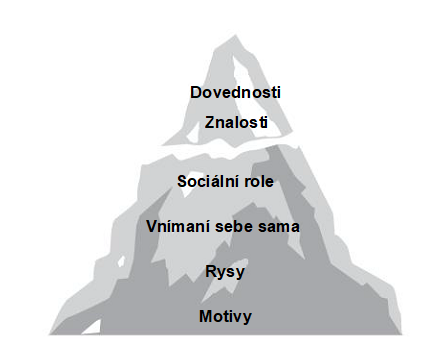
\includegraphics[width=0.65\linewidth]{competence_structure.png}
	\caption{Složení kompetencí znázorněná pomocí ledovce (zdroj \cite{cite:02})}
	\label{fig:competence_structure}
\end{figure}

\section{Znalosti a dovednosti}
Znalosti a dovednosti jsou ze všech složek  kompetencí nejlépe uchopitelné. To však není, vzhledem k jejich komplexnosti, nijak uspokojivé. Důvodem je, že u nich lze předpokládat, že je buď sám vlastník umí popsat, nebo je možné je poměrně jednoznačně vyčíst z jeho činů (např. z jeho vědeckých prací, z potvrzených referencí zaměstnavatelem). Na rozdíl od rysů, motivů a sociálních rolí (obr. č. \ref{fig:competence_structure}), které ani samotný vlastník často nedokáže přesně definovat.\par
Je tedy velmi pravděpodobné, že optimální cesta za vyhledáváním dle kompetencí povede okolo znalostí a dovedností. Pro začátek si je definujeme.
\subsubsection*{Znalost}
 Pochopení určité informace, které osoba získá zkušeností nebo studiem. \cite{cite:01} (přeložil autor) \par
\paragraph{Typy znalostí:}
\begin{itemize}
\item Deklarativní
\begin{itemize}
\item Popisují, jaké věci známe a co o nich víme; např. pes je zvíře, pes má ocas
\item Mohou být popsány pomocí grafů a podobných struktur
\end{itemize}
\item Procedurální
\begin{itemize}
\item Popisují, jak věci fungují, např. jestliže je pes hladový, najde si jídlo a sní ho
\item Mohou být popsány pomocí pravidel \cite{cite:11}
\end{itemize}
\end{itemize}
Znalosti ještě v kontextu jejich vyvozování dělíme na \textit{explicitní} a \textit{implicitní}.  \textit{Explicitní} znalosti jsou znalosti, které byli objektu (počítači, osobě) přímo sděleny, libovolnou formou. \textit{Implicitní} znalosti je poté objekt schopen sám vyvodit na základě znalostí explicitních (např. pomocí logiky).\cite{Stephan2007}\par
Často používaným pojmem je \textit{znalostní báze}, která se nejčastěji pojí k nějakému seskupení lidí, komunitě, popř. k jinému jednotícímu prvku. V podstatě se jedná o množinu znalostí a jejich propojení, které se vztahují ke zvolené jednotící entitě např. firmě, vědeckému výzkumu, nebo i k určitému vědnímu oboru. Například součástí znalostní báze oboru informatika by mohly být všechny známé pojmy s jejich definicemi, propojené různými sémantickými vazbami (nadřazenost, podřazenost, souvislost a jiné).
\subsubsection*{Dovednost}
Dovednost je učením a praxí získaná dispozice ke správnému, kvalitnímu, rychlému a úspornému vykonávání určité činnosti vhodnou metodou \cite{cite:03}. Jinými slovy je to schopnost využít znalosti efektivně k vykonávání určité činnosti \cite{cite:04}.
\section{Další pojmy}
\subsection*{Osoba}
V kontextu této práce je osoba jakýkoliv člověk.
\subsection*{Pracoviště}
Pracoviště je v kontextu této práce seskupení osob. Obvykle má název, místo působení a vedoucí osobou. Dále se dělí na týmy, které pracují společně na cílech definovaných vedoucím.\par
V této práci pojednáváme o vyhledávání osob a pracovišť dle kompetencí. Proto je nutné definovat, co znamená pojem kompetence pracoviště. Pracoviště je kompetentní k určitému předmětu kompetence v případě, že je kompetentní osoba, která je jeho součástí. Váha dané kompetence pracoviště je potom určena součtem váh dané kompetence přes všechny osoby na daném pracovišti.
\subsection*{Data}
Fakta či fikce zapsané v čitelné podobě, čitelné pro stroje či lidi.
\subsection*{Informace}
Informace jsou data o něčem nebo o někom. Jinými slovy jsou to data, která mají daný význam.
% \subsection*{Databáze kompetencí}
% Systém pro ukládání pracovišť, osob a jejich kompetencí, navržený takovým způsobem, který optimálně vyhovuje pozdějšímu efektivnímu zpracování těchto dat (např. vhodná reprezentace). Zpracováním je myšleno: vytváření, čtení (vyhledávání), editace, mazání.\par
% Databáze kompetencí musí mít vždy pevně definovanou množinu osob, kteří se v ní nacházejí (např. zaměstnanci konkrétní organizace, vědecké týmy, akademičtí pracovníci).
\subsection{Jazyk} \label{sec:jazyk}
Obecný jazyk definujme jako prostředek komunikace mezi dvěma a více objekty, nebo jejich částmi. Jazyk je používán k reprezentaci informací.
\subsubsection*{Přirozený jazyk}
Znaky, symboly, zvuky a metody předávání informací, pocitů nebo nápadů.\cite{cite:05} Tento jazyk se vyvinul postupně a přirozeně jako způsob komunikace mezi lidmi.\cite{cite:07}  
\subsubsection*{Formální jazyk}
Tento jazyk je určený pro situace, kdy přirozený jazyk nestačí např. v matematice, logice a informatice. Symboly a vzorce mají mezi sebou přesně definované syntaktické a sémantické vztahy. \cite{cite:07}\par
Přesná syntaxe a sémantika jsou důvodem, proč jsou tyto jazyky obecně v oborech jako je informatika upřednostňovány. Na rozdíl od přirozeného jazyka není formální jazyk tolik zatížen následujícími vlastnostmi:
\begin{itemize}
\item \textbf{Nejednoznačnost} - formální jazyky jsou navrhovány tak, aby buď minimálně nebo vůbec neobsahovali nejednoznačné symboly a vzorce
\item \textbf{Redundance} - pro vyrušení nejednoznačnosti přirozené jazyky zapojují redundanci (popisují jednu skutečnost více způsoby); formální jazyky se tomuto vyhýbají a díky tomu jsou stručnější
\item \textbf{Literárnost} - ve formálních jazycích neexistují idiomy, metafory a podobné jevy \cite{cite:08}
\end{itemize}
Výše zmíněné vlastnosti obvykle přirozený jazyk má, tím pádem je obtížně použitelný v informatice, matematice a podobných oborech.
\section{Shrnutí}
Na první pohled se může zdát, že vysvětlené pojmy spolu příliš nesouvisí. Později se v této práci budeme k některým zmíněným pojmům vracet, případně je budeme již jen používat. Přestože některé pojmy nezmíníme explicitně, v této kapitole mají své místo, tvoří totiž teoretický podklad pro lepší pochopení celé problematiky.

%TODO obrázek pro ilustraci provázanosti pojmů

%ZBYTKY
% \subsection*{Slovo}
% Základní jednotka přirozeného jazyka. \cite{cite:05}
    % \chapter{Datový model}
% Chceme-li dle kompetencí vyhledávat je třeba definovat, jaká data potřebujeme. Druhá neméně důležitá otázka je, jak nejlépe tyto data reprezentovat v strojově čitelné podobě. Na obě tyto otázky se pokusíme odpovědět v této kapitole.
\chapter{Konceptuální datový model} \label{chap:data_model} 
V následující kapitole rozebereme zkoumanou doménu. Tím mimo jiného odpovíme i na otázku \textit{Která data potřebujeme?} (definovanou v kapitole č. \ref{chap:decompisition}).
Ujasníme si, které entity se v naší doméně vyskytují, jaké mají vlastnosti a jaké jsou mezi nimi vztahy.\par 
\noindent Ze zadání vyplývají základní řešené entity – osoby, pracoviště, kompetence. 
% Všechny tyto se vždy vztahují k dané organizaci, ve které vytváříme databázi kompetencí.
\section{Osoby}
% Osoby .
% Uvádíme i atributy, které se obecně považují za osobní údaje. Tyto údaje jsou typicky uchovány v interní databázi organizace a není třeba s nimi manipulovat. Pro naše účely poslouží jen obecný identifikátor v rámci organizace.
% \par
\paragraph{Vlastnosti:}
\begin{itemize}
\item Identifikátor v rámci organizace
\item Jméno
\item Příjmení
\item Pracoviště
\item \textit{Abstraktní hodnocení} - vědecké (např. h-index), pracovní (roky zkušeností) a jiné
\item Znalosti a dovednosti
\item Osobnost - společenské vnímáni, vnímání sebe sama (viz obr. č. \ref{fig:competence_structure} pod hladinou)
\end{itemize}
\section{Pracoviště}
% Jedná se o množinu osob s definovaným vedoucím.\par
\paragraph{Vlastnosti:}
\begin{itemize}
\item Identifikátor v rámci organizace
\item Název
\item Skupina osob
\item Vedoucí
\end{itemize}
\section{Kompetence}
Kompetence je klíčovým prvkem naší domény, její popis je úzce provázán s její reprezentací. To je důvod, proč nemusí být na první pohled zjevné, jak budou její atributy vypadat. Jedná se však jen o konceptuální model, podrobnosti týkající se reprezentace těchto dat připojíme v pozdějších kapitolách. \par
\paragraph{Vlastnosti:}
\begin{itemize}
\item Formální název popř. popis
\item Zdroje - znalosti/dovednosti, povahové rysy (viz obr. č. \ref{fig:competence_structure})
\end{itemize}
\section{Diagram konceptuálního modelu}
Diagram (příloha č. \ref{fig:conceptual_appendix}) zobrazuje vztahy entit mezi sebou a násobnosti těchto vztahů. \par
\noindent Levá část diagramu týkající se osobnosti je pouze schematicky naznačena bez hlubšího rozebrání její vnitřní struktury. Tuto část bereme spíše jako tzv.~\textit{černou skřínku}, neuváděli jsme ani násobnosti vazeb.\par
Cílem konceptuálního modelu je co nejlépe zachytit naší interpretaci skutečnosti. Interpretací může existovat nespočet, tento náš model je výsledkem několika iterací.\par
% Jedná se pouze o konceptuální model, jde tedy výhradně o model interpretace reálného světa, ne o technickou reprezentaci.
% \begin{figure}[htbp!]
% 	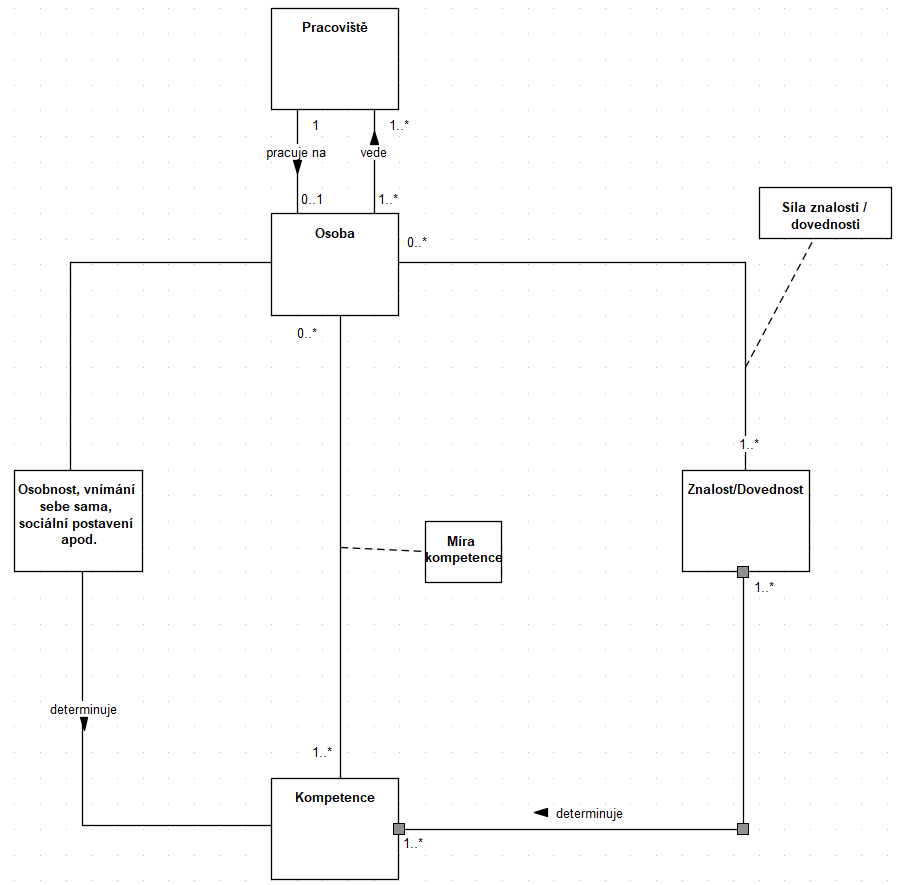
\includegraphics[width=\linewidth]{img/data_diagram.png}
% 	\caption{Diagram konceptuálního modelu}
% 	\label{fig:conceptual_inline}
% \end{figure}
\section{Shrnutí}
Účelem této sekce bylo odpovědět na otázku \textit{Která data potřebujeme?}. Víme, že budeme muset získávat data o osobách, pracovištích a kompetencích. Přibližně víme i jaké atributy můžeme u těchto entit očekávat, z čeho se dále skládají a jaké jsou mezi nimi vazby. Nedozvěděli jsme se přesnou povahu dat, například jejich formu, to rozebereme až v následujících kapitolách.


    \chapter{Reprezentace dat} \label{chap:data_representation}
V této kapitole odpovíme na otázku \textit{Jak budeme data ukládat?}. Rozebereme tedy možnosti reprezentace jednotlivých entit z konceptuálního modelu (obr. \ref{fig:conceptual_appendix}). V závěru této sekce bude jasné, která reprezentace je pro náš případ nejvhodnější a proč.\par
Některé entity z konceptuálního modelu je možné reprezentovat poměrně jednoduše~-~osoby a pracoviště. Stačí nám na to objektové paradigma \cite{Wegner:object_oriented}, které se obvykle při modelování systémů používá.\par
Naproti tomu pracujeme s kompetencemi, znalostmi, dovednostmi a osobností. Modularita těchto entit je větší než u osob a pracovišť. Reprezentovat je klasickým objektovým způsobem může být velmi komplikované. U těchto entit je třeba jít do většího detailu. Reprezentaci osob a pracovišť můžeme později přizpůsobit dle zvolené reprezentace ostatních entit.\par
% \paragraph{Dílčí otázky}:
% \begin{itemize}
%     \item [] \textit{U kterých entit rozebereme reprezentaci dopodrobna?}
%     \item [] \textit{Jaké jsou varianty reprezentace těchto entit a jaké jsou jejich klady a zápory?}
%     \item [] \textit{Jaké existují praktické realizace - implementované formální jazyky, notace apod.?}
% \end{itemize}

\section{Kompetence}
Kompetence osoby, jak je vidět z konceptuálního modelu (příloha \ref{fig:conceptual_appendix}), podmiňují dva vlivy, osobnost a znalosti (resp. dovednosti). Tyto dvě oblasti určují jaké kompetence daná osoba má a v jaké míře.\par
\subsection{Vymezení}
Reprezentace osobnosti tvoří velmi komplikovanou problematiku, na toto téma odkážeme v sekci budoucí práce (kapitola \ref{future}), jelikož stojí za další zkoumání. V této práci se tímto však nebudeme více zabývat, místo toho se zaměříme na znalosti.\par
Omezíme se na reprezentaci kompetencí pomocí znalostí a dovedností a připodobníme míru kompetence k síle znalosti popř. dovednosti, z diagramu (příloha \ref{fig:conceptual_appendix}). 
% Přestože se jimi nebudeme přímo zabývat, budeme v této práci stále brát v úvahu pozdější rozšiřitelnost o další vlivy na kompetence.
\par
Dále problematiku zúžíme pouze na znalosti, jelikož z definice dovednosti plyne, že je závislá na znalosti. Není správné dovednosti úplně vyloučit, i na ně odkážeme v kapitole budoucí práce (kapitola \ref{future}). Společně se zkušenostmi by měly být dalším důležitým okruhem, který staví na znalostech a mimo jiné popisuje, jak je osoba umí využívat.\par
Otázku jsme tedy zúžili z reprezentace kompetencí na reprezentaci znalostí, na tu se zaměříme v další sekci.
\section{Znalosti} \label{sec:knowledge_representation}
Reprezentace znalostí (angl. \textit{knowledge representation}) je společně s uvožováním (angl. \textit{reasoning}) prudce se rozvíjejícím oborem umělé inteligence. V této sekci popíšeme, co vůbec reprezentace znalostí je a představíme si vybrané formální jazyky, které pro tuto reprezentaci lze využít (v některých zdrojích se mluví o formalismech, v jiných o formách, my jim budeme říkat formální jazyky, protože, to je zdaleka nejjednoznačnější pojmenování).
\subsubsection{Co je reprezentace znalostí}
Dříve než přistoupíme ke konkrétním formálním jazykům, musíme si ujasnit termín reprezentace znalosti. Reprezentace znalostí se dá shrnout do čtyř základních charakteristik:
\begin{itemize}
\item Náhrada reality
\item Množina ontologických závazků
\item Fragmentární teorie inteligentního uvažování
\item Prostředek pro počítač i člověka \cite{cite:09}
\end{itemize}
\subsubsection{Náhrada reality}
Pod touto charakteristikou leží základní filozofický předpoklad, že realita existuje nezávisle na jakémkoliv pozorovateli - počítači, člověku aj.\par
Náhrada reality, tedy reprezentace znalosti, nám umožňuje uvažovat a modelovat situace. Základem uvažování je vyvozování závěrů bez samotných činů. Příkladem může být plán stavby domu. Aniž bychom do ruky vzali jediný nástroj či materiál, jsme schopni dům zkonstruovat v rozsahu svých znalostí pouze ve vlastní hlavě.\par
Kvalita a rozsah naší reprezentace se vždy odvíjí od přesného účelu, pro který znalosti používáme/uchováváme. Je velmi nepravděpodobné, že by se nám podařilo reprezentovat naprosto všechno bez rozdílu od reality, je proto důležité vědět, jak moc a čím se reprezentace od reality liší.\cite{cite:10}
\subsubsection{Ontologické závazky} \label{ontological_commitments}
Předpokládáme, že nelze reprezentovat vždy všechno, každá reprezentace je v podstatě jen aproximací reality. Reprezentaci volí sám pozorovatel, tím dělá rozhodnutí, které znalosti bude reprezentovat a jak. Volba nejpříhodnější reprezentace je tedy množinou takových rozhodnutí - přesněji ontologických závazků.\cite{cite:09}
\subsubsection{Fragmentární teorie inteligentního uvažování}
Reprezentace znalostí je známka inteligentního chování. Existují nejméně dva pohledy na to, co je inteligentní chování. První z nich odkazuje na logiku a říká, že cokoliv, co se chová podle logických pravidel, je inteligentní. Druhý pohled nahrazuje logická pravidla množinou mechanizmů inspirovaných procesem poznáváním.\cite{cite:10} \par 
Oběma těmito přístupy se existující formální jazyky inspirují, některé využívají logiku, některé proces poznávání. \cite{cite:10}
\subsubsection{Prostředek pro počítač i člověka}
Počítačové zpracování znalostí reprezentovaných formálními jazyky pro to určenými musí být efektivní. Často platí, že čím je jazyk složitější, tím je složitější jej zpracovat.\cite{cite:10} \par 
Naproti tomu musí být jazyk dobře pochopitelný pro člověka. Zde se nabízí přirozený jazyk, ten však díky svým vlastnostem (kapitola č. \ref{sec:terms} sekce č. \ref{sec:jazyk}) není vhodný. Bude-li jazyk špatně pochopitelný pro člověka, nebude možné rychle ověřit pravdivost/důvěryhodnost sdělení vyjádřeného pomocí tohoto jazyka. Takový jazyk vědecká ani komerční komunita nepřijme. \cite{cite:10}

\section{Formální jazyky pro reprezentaci znalostí}
V této sekci shrneme existující formální jazyky pro reprezentaci znalostí. Každý z nich zevrubně popíšeme, abychom v závěru této kapitoly mohli rozhodnout, který se pro naše účely hodí nejvíce.

% \subsection{Rozdělení formálních jazyků}
% Formální jazyky pro reprezentaci znalostí lze rozdělit na dvě skupiny - \textit{logic-based} a \textit{non-logic-based}. (nevhodné překládat z angličtiny)\par
% \textit{Non-logic-based} jazyky nemají tak silné sémantické hranice, dá se říci, že jsou "méně formální". Jedná se například o sémantické sítě (popsány níže).\par
% % Naproti tomu \textit{Logic-based} mají díky logice sémantiku přesně danou. Můžeme tedy říct, že z hlediska vlastností formálních jazyků, popsaných v sekci \ref{sec:jazyk}, jsou "více formální". Jedná se například o jazyk ALC - jazyk deskripční logiky. (popsán níže) \par
% Speciálním případem jsou ontologie, které rozebíráme v dalších sekcí. Ontologie, jelikož staví na základech více jazyků pro reprezentaci znalostí, mají úroveň "formálnosti" modulárnější. Tato "formálnost" se často odvíjí od konkrétního případu užití a zvoleného způsobu řešení. 
\subsection{Sémantické sítě}
Sémantická síť je graf, jehož uzly reprezentují koncepty a individuality, hrany potom reprezentují vztahy mezi nimi.\cite{cite:10}\par
\begin{figure}[htbp!]
	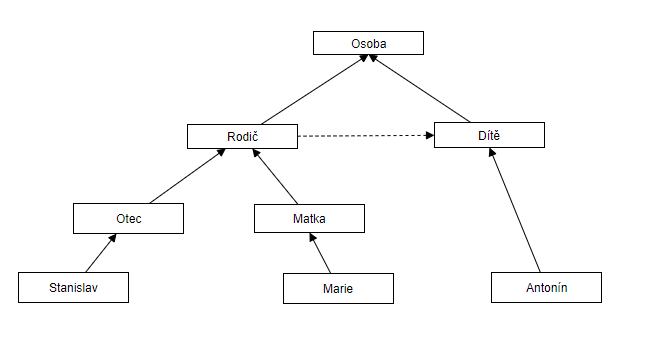
\includegraphics[width=0.8\linewidth]{img/semantic_network.png}
	\caption{Příklad sémantické sítě popisující některé rodinné vztahy (zdroj \cite{Stephan2007}, přeložil autor)}
	\label{fig:semantic_network}
\end{figure}
\noindent \textbf{Individuality} reprezentují konkrétní objekty ze zkoumané domény, na obrázku č. \ref{fig:semantic_network} jsou to např. otec Stanislav nebo dítě Antonín.\par
\noindent \textbf{Koncepty} jsou množiny individualit. Na obrázku č. \ref{fig:semantic_network} jsou to např. rodič a osoba, které reprezentují všechny rodiče a všechny lidi ve sledované doméně.\cite{cite:10}\par
\par Každý uzel má své vlastnosti, jsou jimi atributy a relace. Atributem může být např. věk u osoby. Základními relacemi jsou IS-A a \textit{instance-of}. Relace IS-A definuje hierarchii konceptů (tvz. taxonomii), v obrázku č.\ref{fig:semantic_network} platí, že matka IS-A rodič. Vztah IS-A indikuje dědění všech vlastností nadřazeného konceptu konceptem podřízeným (např. matka dědí všechny vlastnosti rodiče). Vztah \textit{instance-of} je vždy mezi konceptem a individualitou, v obr. č. \ref{fig:semantic_network} platí Stanislav \textit{instance-of} otec.\cite{cite:10} Nejedná se samozřejmě o všechny druhy vazeb, jen o ty klíčové.\par
Sémantické sítě se nejčastěji používají pro modelování deklarativních znalostí, lze je však použít i pro procedurální znalosti.\cite{cite:11}\par
Původní význam slova \textit{sémantická sít} je \textit{fyzický model lidské paměti} \cite{cite:12}. Sémantické sítě se člověku snadněji chápou a práce s nimi je přirozenější než u dalších modelů, hlavně u těch logických.\par
Nevýhodou sémantických sítí je, že neexistuje jednotný standard pro interpretaci a jednotný standard pro hodnoty uzlů a hran - tedy neexistuje jednotná sémantika. Další nevýhodou je dědičnost, která nepodporuje žádné výjimečné stavy (např. tučňák je pták, tedy měl by mít všechny vlastnosti ptáků, ale nelétá). \cite{cite:12}
\subsection{Rámce}
Síť rámců (angl. frames) lze považovat za jeden z typů sémantických sítí. Vedle deklarativních znalostí, které reprezentuje obecná sémantická síť, reprezentují rámce i procedurální znalosti.\par
Základním stavebním kamenem této sítě jsou rámce. Ty v sobě uchovávají proceduru a skupinu atributů, které popisují danou situaci. Rámce se inspirují v lidské paměti, která si uchovává situace - kombinace procedurálních a deklarativních znalostí. Tak může lidský mozek například na dvě, na první pohled rozdílné, situace reagovat stejným způsobem, protože nalezne podobnost.\cite{cite:11}\par
Rámce řeší některé nedostatky sémantických sítí jako je: řešení výjimečných stavů, kontrola vnitřní konzistence a zamezení konfliktům atributů při dědičnosti. Hlavní nevýhodou je složitost použití.\cite{cite:12}
\subsection{Pravidla}
Deklarativní i procedurální znalosti lze reprezentovat jako množinu pravidel. Typický tvar těchto pravidel je tzv. JESTLIŽE-PAK (angl. IF-THEN), například \textit{jestliže je nalezena odpověď, pak jí přestaň hledat, jinak pokračuj v hledání}\cite{cite:11}. Takovou reprezentaci využívají např. logické programovací jazyky.\cite{cite:12}\par
Výhodou pravidel je, že jsou modulární a zároveň jsou poměrně prostorově nenáročná. Jednotlivá pravidla mohou být přidávána a odebírána bez ovlivnění zbylých. Mezi nevýhody patří hlavně složitost odhalení rozporu mezi pravidly a složitost reprezentace složitějších strukturovaných znalostí (svazuje nás přesná forma). V neposlední řadě je velmi složité předpovědět akce, které na základě pravidel nastanou, a tak se pravidla mohou nekonečně řetězit.\cite{cite:12}\par
Pravidla se samozřejmě (např. v programovacích jazycích) aktivně využívají, ale nehodí se pro reprezentaci komplexních znalostí. V programovacích jazycích se používají velmi hojně pro řízení toku programu, ale oproti reprezentaci celé zkoumané domény znalostí je to stále poměrně málo.
\subsection{Logika}
Logika mezi ostatními formálními jazyky pro reprezentaci znalostí převládá \cite{Stephan2007}. V této sekci projdeme klíčové koncepty logiky, nejdříve se zaměříme na obecnou rovinu, poté popíšeme více do detailu deskripční logiku.\par
Logika má mnoho forem, některé z nich se používají, nebo alespoň byly použity, pro reprezentaci znalostí. \cite{cite:12} Jen některé z těchto vyzkoušených forem se osvědčily. \par
V předchozích způsobech reprezentace, zejména potom u sémantických sítí, chyběla jednotně definovaná sémantika, proto je velmi komplikované tyto způsoby přímo aplikovat. \cite{Stephan2007} Znalosti vyjádřené pomocí sémantických sítí mohou být jednoduše vyjádřeny formou logiky, která sítím přidává potřebnou sémantiku. \cite{cite:12}\par
\noindent Následující dvě zobrazení reprezentují totéž:\par
\vspace{3mm}
\noindent\fbox{Zaměstnanec} $\xrightarrow{\text{\textit{je druhem}}}$ \fbox{Osoba} \indent
$\forall x: (Zaměstnanec(x) \to Člověk(x))$
\par\vspace{4mm}
\noindent Stejně jako je tomu u sémantických sítí, tak i u logiky platí, že jsme pomocí ní schopni vyjádřit naprostou většinu přirozeného jazyka. Je důležité si uvědomit, že přestože má logika v sémantice navrch nad sítěmi, sítě jsou intuitivnější pro lidské chápání. \par
Formální jazyky založené na logice obvykle zakládají na logice prvního řádu (predikátové logice), zkratka FOL.\cite{cite:12}\par

\subsubsection{Deskripční logika}
Deskripční logika je natolik expresivním jazykem, že se v dnešní době stala nejčastějším logickým paradigmatem pro reprezentaci znalostí, zejména potom v sémantickém webu. \cite{Stephan2007}.\par
Deskripční logika je téměř výhradně podmnožinou logiky prvního řádu (FOL), tedy logiky predikátové \cite{Stephan2007}. FOL popisuje doménu pomocí objektů (entity mající vlastní identitu), okolo těchto entit jsou konstruovány, pomocí funkcí, proměnných a logických spojek, logické vzorce (predikáty) \cite{Russell:2009:AIM:1671238}. Deskripční logika je typicky omezena pouze na unární a binární predikáty z FOL. \cite{Stephan2007}\par
\paragraph{Základními konstrukty jsou:}
\begin{itemize}
\item Atomické koncepty
\begin{itemize}
\item reprezentují pojmenované unární predikáty
\item např. \textit{Rodič}
\end{itemize}
\item Atomické role
\begin{itemize}
\item reprezentují pojmenované binární predikáty
\item např. \textit{má dítě, je dítětem}
\end{itemize}
\item Individuality
\begin{itemize}
\item reprezentují prvky konceptů, tzn. jednotlivce
\item např. \textit{Jiří} \cite{Kremen2011}
\end{itemize}
\end{itemize}
\paragraph{Znalostní báze většiny deskripčních logik se skládá z \cite{Stephan2007}:}
\begin{itemize}
\item \textit{T-Box} - reprezentuje axiomy obecně platné v dané doméně
\begin{itemize}
\item např. \textit{Muž je osoba}
\end{itemize}
\item \textit{A-Box} - reprezentuje konkrétní relační strukturu
\begin{itemize}
\item např. \textit{Jiří je muž} \cite{Kremen2011}
\end{itemize}
\end{itemize}
Jednotlivé deskripční logiky se liší v možnostech tvořit složitější koncepty případně role a v typech axiomů \cite{Kremen2011}.
Jeden z nejdůležitějších a nejpoužívanějších jazyků deskripční logiky je ALC. \cite{Stephan2007}

\section{Ontologie} \label{ontologies}
Všechny jazyky pro reprezentaci znalostí, které nejsou založeny na logice mají své nedostatky. Nejčastěji je problém v nedostatku sémantiky. Logika těmto jazykům potřebnou sémantiku dodala a můžeme jí díky tomu prohlásit za nejpřesnější způsob, jak znalosti formálně reprezentovat. (ne nutně nejefektivnější)\par
V této sekci přejdeme od konkrétních jazyků ke komplexnějšímu pohledu na reprezentaci znalostí. Ontologie lze také považovat za formální jazyk reprezentace znalostí. Jsou  však spíše realizací předchozích formálních jazyků než-li nový teoretický pohled na reprezentaci znalostí.\par
\subsection{Význam a Definice}
Význam slova ve filozofii odkazuje na tzv. "jsoucno", tedy zkoumání existence. Se zkoumáním existence úzce souvisí otázka: \textit{Co existuje?}. K odpovědi na tuto otázku je nutný systematický postup. Potřebujeme definovat tzv. ontologické kategorie, do kterých všechny zkoumané objekty rozdělíme. Příkladem takových ontologických kategorií mohou být: \textit{lidé, zvířata, věci}. Konkrétní existující instance 
% (nazveme je \textit{individuality} jako v případě předchozích formálních jazyků) 
jsou potom např. \textit{člověk Jiří, pes Alík, česká královská koruna}. Přesně z této ideje ontologických kategorií vychází význam slova ontologie v počítačových vědách. \cite{Stephan2007} Nejedná se tedy o stejné zkoumání jako v případě filosofie, ale stále se pohybujeme ve stejné oblasti.\par
Ontologickými kategoriemi obecně určujeme, které znalosti budeme schopni reprezentovat - určujeme specifickou doménu, pro kterou znalosti modelujeme. Tvoříme tak tzv. \textit{ontologický slovník}.\par
% Zde je možné najít souvislost s ostatními formálními jazyky - ontologie v podstatě popisují názvy hran v sémantických sítích, popř. logické vzorce, používané pro reprezentaci znalostí.\cite{Stephan2007}\par
Obecně ontologie tedy popisují, co v dané doméně existuje. Ontologie jako konkrétní počítačový artefakt (např. soubor) kóduje danou znalost o doméně v počítačem zpracovatelné formě.\cite{Stephan2007}\par
\noindent Doslovná definice ontologie dle \cite{gruber1993translation} je:\par
\begin{quote}
    \textit{Ontologie je explicitní specifikace konceptualizace.}
\end{quote}\par
\noindent Později byla tato definice rozšířena dle \cite{Borst97} na:\par
\begin{quote}
    \textit{Ontologie je formální specifikace sdílené konceptualizace.}
\end{quote}\par
\subsection{Základní charakteristiky}
\begin{enumerate}
\item Formální
\begin{itemize}
\item Ontologie musí být vyjádřena formálním jazykem (výhody těchto jazyků jsou popsány v kapitole č. \ref{sec:terms} sekce č. \ref{sec:jazyk}).
\end{itemize}
\item Explicitní
\begin{itemize}
\item Znalost musí být vyjádřena maximálně explicitně, pro optimální strojové zpracování.
\end{itemize}
\item Sdílené
\begin{itemize}
\item Ontologie vždy reflektuje dohodu skupiny lidí v dané doméně, v podstatě se jedná o kolektivní ontologické závazky (viz sekce č. \ref{ontological_commitments}).
\end{itemize}
\item Konceptuální
\begin{itemize}
\item Ontologie popisuje znalosti pomocí symbolů, které reprezentují koncepty a relace mezi nimi. Konceptualita spočívá v tom, že jsou ontologie intuitivně uchopitelné pro člověka, protože odpovídají lidskému mentálnímu modelu znalostí. Jako protipříklad lze uvést neuronové sítě, které též reprezentují určité znalosti, ale přirozenému lidskému chápání je to již vzdáleno.
\end{itemize}
\item Doménově specifická
\begin{itemize}
\item Ontologie je vždy omezena na určitou oblast - doménu.\cite{Stephan2007}
\end{itemize}
\end{enumerate}

% Ontologie jsou v praxi používány v informačních systémech pro rozhodování a vyvozování (angl. reasoning) v dané doméně.\cite{Stephan2007}\par

\subsection{Základní stavební kameny}
\begin{itemize}
\item Koncepty
\begin{itemize}
\item V sémantických sítích i v deksripční logice se tento konstrukt nazývá stejně
\item Reprezentují ontologické kategorie
% \item V příloze na obrázku č. \ref{fig:ontology_example} např. City
\end{itemize}
\item Relace
\begin{itemize}
\item Analogicky se jedná o hrany sémantické sítě nebo role v deskripční logice
\item Propojují koncepty a instance - reprezentují vazby mezi nimi
% \item V příloze na č. \ref{fig:ontology_example} např. locatedIn
\end{itemize}
\item Instance
\begin{itemize}
\item Individuality v sémantické síti nebo v deskripční logice
\item Reprezentují konkrétní objekty v doméně \cite{Stephan2007}
% \item V příloze na obrázku č. \ref{fig:ontology_example} např. Berlin
\end{itemize}
\end{itemize}
%Ontologii si lze také představit jako množinu výroků (axiomů) např. \textit{OsobaX je člověk} apod.  \cite{Stephan2007}\par
\subsection{Zápis ontologií}
Ontologie lze zapisovat několika způsoby. Například pomocí sémantických sítí, které typicky neobsahují všechny důležité informace, jelikož nejsou tak expresivní (viz sekce č. \ref{fig:semantic_network}). Toto zobrazení je příznivé hlavně pro pochopení lidmi. Dále je zapisujeme pomocí serializovaného formátu (např. XML), vhodného pro strojové zpracování. Dále pomocí logických vzorců, to je vhodné pro další vyvozování (angl. reasoning). \cite{Stephan2007}.

\subsection{Použití ontologií}
\begin{itemize}
\item \textbf{Propojení znalostí} - jednotný znalostní slovník napříč aplikacemi, datový zdroj znalostí
\item \textbf{Abstrakce znalostí} - zdroj schématu znalostí (hierarchie a vztahy konceptů) pro budoucí využití
\item \textbf{Automatizace zpracování znalostí} - automatické vyvozování závěrů z platných axiomů (angl. reasoning)
\item \textbf{Integrace informací} - integrace na úrovni různých datových schémat a interpretace získaných dat z jednoho zdroje v rozdílném schématu
\item \textbf{Získávání informací} - zdokonalování modelu znalostí s důrazem na jeho prohledávání
\item \textbf{Sémantická správa obsahu} - přidávání metadat k datům, která později slouží k jejich lepší identifikaci a lepšímu přístupu k nim
\item \textbf{Organizace znalostí} - sdílený znalostní model daného seskupení lidí (např. firma, škola)
\item \textbf{Expertní systémy} - systémy schopné řešit komplikované otázky (úlohy) - např. i v medicíně \cite{Stephan2007}
\end{itemize}
\subsection{Typy ontologií}
Existují čtyři základní typy ontologií. Jednotlivé typy se od sebe liší úrovní abstrakce reprezentovaných znalostí. \cite{Stephan2007}\par
\begin{itemize}
\item \textbf{Top-level}
\begin{itemize}
\item Abstraktní a obecné koncepty (např. \textit{fyzický objekt, abstraktní objekt}) s velkým potenciálem znovupoužití v mnoha doménách
% \item typicky se přímo nenachází v aplikacích - spíše ontologie, které se jimi řídí
\item Typicky se používají jako předloha pro tvorbu ontologií zmíněných níže
\item Příklady UFO \cite{Guizzardi2005}, SUMO \cite{Niles:2001:TSU:505168.505170}, DOLCE \cite{Dolce}
\end{itemize}
\item \textbf{Doménové a úkolové ontologie}
\begin{itemize}
\item Zachytávají znalost ve specifické doméně - např. medicíně, geografii; nebo znalost o specifickém úkolu - např. diagnostika, konfigurace
% \item Doménové ontologie se zaměřují na "statické" znalosti o doméně, úkolové potom na postupy, plánování, monitoring apod. - "dynamické" znalosti
\end{itemize}
\item \textbf{Aplikační ontologie}
\begin{itemize}
\item Propojují doménové a úkolové ontologie pro účely konkrétní aplikace
\end{itemize}
\end{itemize}
Jedná se o inkluzivní hierarchii, nižší ontologie přejímají a konkretizují obecné koncepty a relace vyšších ontologií. \cite{Stephan2007}
\begin{figure}[htbp!]
	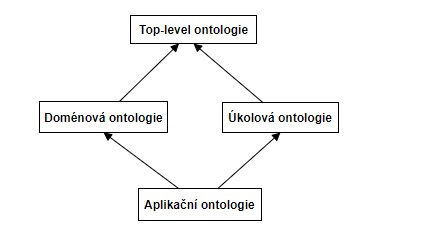
\includegraphics[width=0.7\linewidth]{img/ontology_types.png}
	\caption{Typy ontologií (zdroj \cite{Stephan2007}, přeložil autor)}
	\label{fig:ontology_types}
\end{figure}


\subsection{Přidružené technologie, standardy a další}
% Existuje několik jazyků, které jsou určené pro zápis a jednoznačnou reprezentaci ontologií ve strojově čitelné formě. Uvedeny jsou pouze ti nejpoužívanější kandidáti.
\subsubsection{RDF}
V doslovném překladu se jedná o framework pro popis zdrojů. RDF je standardizovaný jazyk pro reprezentaci znalostí (informací) na webu. Tento jazyk lze však použít pro reprezentaci libovolných znalostí.\par
\paragraph{Základními elementy jsou:}
\begin{itemize}
\item URI (Uniformní identifikátor zdroje) - slouží k pojmenování a identifikaci individualit, konceptů a jejich vlastností (příklad je \textit{urn:isbn:0451450523}, což je URI knihy)
\item Věty ve tvaru: \fbox{Podmět} $\xrightarrow{\text{\textit{Predikát}}}$ \fbox{Předmět} (jednotlivé členy jsou ve tvaru URI)
% \begin{itemize}
% \item []\textbf{Příklad} \fbox{http://web.de/MrX.html}$\xrightarrow{\text{\textit{btr:maAutora}}}$ \fbox{btr:PanX} \cite{Stephan2007}
% \end{itemize}
\end{itemize}
RDF je typicky zpracováváno v serializované podobě v XML formátu (viz příklad níže) \cite{Stephan2007}. Poměrně populární variantou pro serializaci RDF je též JSON-LD \cite{JSON_LD} nebo Turtle \cite{TURTLE}.\par

\begin{lstlisting}[caption= Příklad syntaxe RDF XML, captionpos=b]
<rdf:Description rdf:about="http://ubiqbiz.com/web/MrX.html">
    <btr:hasAuthor rdf:resource="btr:PanX"/>
</rdf:Description>
<rdf:Description rdf:about="btr:PanX">
    <btr:employedAt rdf:resource="btr:UbiqBiz"/>
</rdf:Description>
\end{lstlisting} 

RDF je framework pro prostý popis zdrojů, pokud chceme datům dávat význam a s tímto významem pracovat, musíme využít další rozšíření. Typicky datům dodáváme soubor axiomů pro další vyvozování (angl. inference) popř. uvažování (angl. reasoning), které nám umožní je dále rozvíjet a efektivně s nimi pracovat. V následujícím seznamu uvádíme příklady takových rozšíření.
\begin{itemize}
\item Vyvozování dalších znalostí, popis schématu
\begin{itemize}
\item \textbf{RDFS} - omezené prostředky na rozdíl od pokročilejších \par(zdroj: \url{https://www.w3.org/TR/rdf-schema/})
\item \textbf{OWL} - ve své podstatě univerzální jazyk pro popis ontologií \par(zdroj: \url{https://www.w3.org/TR/owl2-primer/}, podrobněji níže)
\end{itemize}
\item Validace modelu
\begin{itemize}
\item \textbf{SHACL} - validace RDFS (zdroj: \url{https://www.w3.org/TR/shacl/})
\end{itemize}
\end{itemize}

\subsubsection{SPARQL}
\noindent Dotazovací jazyk standardizovaný pro vyhledávání a další operace v RDF \cite{SPARQL}.\par
\subsubsection{OWL}
\noindent Web Ontology Language (OWL) je  standardizovaným jazykem pro sémantickou anotaci webového obsahu. Jazyk má 3 varianty, my se zaměříme pouze na nejčastěji používanou a to je OWL-DL (z angl. \textit{OWL description logic}).\par
Syntaxe OWL zakládá na RDF a rozšiřuje jej. Větám (trojicím) dává ve své podstatě další sémantiku, kterou lze později interpretovat.\par
% \paragraph{Základními konstrukty jsou:}
% \begin{itemize}
% \item Třídy (koncepty z DL)
% \item Vlastnosti (role z DL)
% \item Individuality (v DL stejně)
% \item Konstruktory tříd (slouží k tvorbě složitějších tříd)
% \end{itemize}
Dokument v jazyce OWL je v podstatě množina výroků, které mohou být interpretovány jako axiomy v deskripční logice. OWL je mocný nástroj, jelikož vychází z deskripční logiky a převzalo její výhody - je možné kontrolovat konzistenci a vyvozovat implicitní znalosti. \cite{Stephan2007}

\subsubsection{OntoUML}
Rozšíření jazyka UML určené pro modelování ontologií. Toto rozšíření je založeno na top-level ontologii UFO \cite{Guizzardi2005}.

\subsubsection{SKOS}
SKOS (z angl. Simple knowledge organization system) je standard pro sdílení strojově čitelných dat. Tento standard řeší základní problém systémů pro organizaci znalostí (zkratka KOS). Tyto systémy operují se znalostmi v různé formě~-~např. obecné slovníky, thesauri, taxonomie, klasifikační schémata. SKOS standardizoval sdílení těchto dat v jednotné formě, která zachovává výhody původních forem (slovníky, thesauri...). Cílem je mít data dostupná v jednotném formátu - RDF. \cite{SKOS}\par 
% OWL Full ontologie \cite{OWL_FULL}.
Standard SKOS klade menší důraz na formálnost, míří více na přímou konverzi dat na znalosti a jejich použití v různých situacích. Neklade takový důraz na uvažování (angl. reasoning) a vysokou přesnost dat. \cite{isaac2009skos}\par 
SKOS je ve své podstatě ontologií, jak je možné vidět na obrázku v příloze \ref{fig:SKOS-ontology}. 

% Bližší specifikace SKOS je dostupná zde https://www.w3.org/TR/2005/WD-swbp-skos-core-guide-20051102/#secabout.\cite{SKOS}

%TODO příklad OWL














\subsection{Reprezentace a datová struktura}
Každá reprezentace je nakonec realizována pomocí některé známé datové struktury. Například u sémantické sítě je to typicky graf. Je důležité striktně dodržovat sémantiku dané reprezentace, která ne vždy platí obecně pro použitou datovou strukturu. Například sémantická síť popisující rodinné vztahy v sobě netoleruje cykly, to ale pro obecný graf neplatí. \cite{cite:09}




% TODO: 
% jednotlivé zhodnotit - napsat vhodné použití apod., zkusit se zaměřit na ohledy vyhledávání v těchto informacích pomocí fulltextu...(snad)



\section{Shrnutí}
Cílem této kapitoly bylo odpovědět na další z dílčích otázek našeho problému: \textit{Jak budeme data ukládat?}. Rozebrali jsme tedy možnosti reprezentace jednotlivých entit a nyní můžeme rozhodnout, která je pro naše účely nejvhodnější.\par 
Je důležité zmínit, že námi zvolený postup jistě není jediný možný. Přestože v této kapitole vybereme jednu z představených možností, nadále budeme pracovat tak, aby naše řešení bylo modulární. Budeme jej navrhovat tak, aby jeho části bylo možné nahrazovat vylepšenými případně změněnými (hlavně při návrhu systému - kapitola č. \ref{chap:app-design}).\par
Klíčovou částí této kapitoly byly formální jazyky pro reprezentaci znalostí. Jazyky byly představeny s vzestupnou tendencí, co se týká praktického použití. První představené, hlavně sémantické sítě, byly lépe pochopitelné pro člověka, ale postrádaly dostatečně definovanou sémantiku pro praktické aplikace. Naproti tomu později představená deskripční logika je kvalitnějším jazykem, jelikož předchozím formálním jazykům dodává zmíněnou potřebnou sémantiku.\par
Nakonec jsme se v této kapitole zabývali ontologiemi. Ontologie jsou více realizací zmíněných formálních jazyků, než že by do této problematiky přinášeli něco úplně nového. Ontologie staví na deskripční logice a přebírají expresivitu tohoto jazyka, zároveň jsou vizualizovány pomocí sémantických sítí, které jsou pro práci přehlednější pro člověka. V kontextu ontologií existují konkrétní jazyky (RDF, OWL) a praktické aplikace (SKOS), které jsou již ověřené.\par
Vzhledem k vlastnostem, které jsme zmínili, jsou ontologie a množina přilehlých technologií v našem případě vhodnou volbou pro reprezentaci znalostí.\par

% Volba ontologie, pro tuto práci, shrnuli jsme však teoretický základ pro další směry
% Zmínit se o osobách a pracovištích

% Následujícím úkolem je zajistit, jak data, která máme k dispozici, transformovat do zvolených reprezentací - ontologií. Této výzvě však předchází ještě analýza datových zdrojů, která by nám měla ukázat, jakou povahu naše data budou typicky mít. Na základě této znalosti budeme schopni rozhodnout o transformaci. Na datové zdroje se zaměříme v další kapitole.

% POZOR - měli bychom si uvědomit nejdříve proč ty data chceme vůbec reprezentovat - to nám v pozdější sekci pomůže říct, co je pro nás lepší (https://www.matthewrenze.com/presentations/transforming-data-into-knowledge.pdf) Náš účel bude data exploration (úzce propojeno s vizualizací.
% \section{Osoby a pracoviště}
% Tyto dvě třídy mají pouze prosté atributy a neměl by být problém je reprezentovat různými způsoby. Osoba samozřejmě vlastní kompetence, znalosti a osobnost, proto bude n


    \chapter{Zdroj dat} \label{chap:sources}
V této kapitole rozebereme další dílčí problematiku, která je součástí našeho komplexního problému - zdroje dat.\par
Nejdříve se zaměříme na zdroje dat o pracovištích a osobách. Poté rozebereme zdroje znalostí s důrazem na strojovou zpracovatelnost.\par

\section{Forma dat a přístup k nim}
Přístup k datům je obvykle realizován pomocí webových rozhraní (tzv. API). Pro komunikaci s tímto API se obvykle využívá protokol HTTP. Velmi často používaným konceptem pro návrh rozhraní je REST \cite{REST}. Rozvíjejícím se dotazovacím jazykem se díky své modularitě stává GraphQL \cite{GRAPHQL}, který operuje také nad zmíněným HTTP protokolem. \par
Přístup k datům je typicky zabezpečen a není možné, aby jej získal kdokoliv. Často je nutné zažádat o přístup a poskytnout přesný účel, pro který data chceme získat. Každý datový zdroj má obvykle svou autentizační proceduru, tu je třeba vyjednat s poskytovatelem dat.\par
Po překonání autentizační procedury jsou data přístupná, obvykle v serializovaném formátu. Nejčastější serializované formáty jsou JSON \cite{JSON} a XML \cite{XML}. V těchto formátech lze serializovat libovolná strukturovaná data například i RDF (viz kapitola č. \ref{sec:knowledge_representation}).\par
Získaná data jsou samozřejmě strukturována dle datového schématu poskytovatele. Pokud se naše schéma liší od schématu poskytovatele, musíme data příslušným způsobem transformovat, tento problém vyřešíme v pozdějších kapitolách. Možností, jak data získat, je nespočet, zmínili jsme jen neobvyklejší metody.

\section{Osoby a pracoviště}
Data o těchto entitách jsou typicky dostupná v databázi/evidenci pracovníků resp. členů daného seskupení (firma, škola aj.). \par
\noindent S daty o osobách je nutno pracovat dle směrnice GDPR \cite{GDPR}.
% Pro účely databáze kompetencí bude nutné o osobách získat následující informace - jméno, příjmení, id v rámci organizace, pracoviště. Tyto informace jsou zmíněnou směrnicí považovány za osobní údaje.




\section{Znalosti} %[TODO: pohovořit o strojovém zpracování dat]
Znalosti mají v databázi kompetencí velmi důležitou roli. Komplexita této entity ve své podstatě určuje i práci s ostatními entitami a fungování celého systému.\par
\noindent V kontextu znalostí musíme vyřešit následující problémy:
\begin{itemize}
    \item Znalosti osob
    \item Znalostní báze
\end{itemize}
% [TODO: rozmyslet, jestli toto nedat ještě do nějaké sekce zvláštní ohledně obecného procesu vyhledávání dle kompetencí a způsobů (viz níže), možná by se to dalo demonstrovat na obrázku]
Při vyhledávání osob dle znalostí můžeme zvolit různé přístupy v závislosti na získávaných znalostech. Identifikovali jsme dvě kategorie řešení:
\begin{itemize}
    \item Se sémantikou - pracuje s významem vyhledávaných konceptů
    \item Bez sémantiky - pracuje na jiném principu, nebere v úvahu sémantiku
\end{itemize}
Na základě tohoto rozdělení můžeme konstatovat, že pokud se jedná o řešení bez sémantiky, z pravidla toto řešení nebude potřebovat znalostní bázi. Jedná se například o fulltextový vyhledávač přes danou sadu dokumentů a jednoduchá interpretace výsledku.\par
V případě řešení se sémantikou je třeba znalostní bázi vytvořit a udržovat. Příkladem takového řešení může být znalostní báze uložená pomocí ontologií a následné vyhledávání konceptů v tomto ontologickém slovníku.\par
\section{Znalosti osob}
Pro vyhledávání osob dle jejich znalostí je třeba tyto znalosti získat. Datový zdroj takových znalostí musí poskytovat minimálně následující atributy:
\begin{itemize}
    \item Osobu
    \item Znalost %(koncept)
    \item Sílu znalosti
\end{itemize}
Znalosti osob je možné získat například z podpůrných systémů dané organizace (systémy pro organizaci znalostí, osobní profily zaměstnanců a jiné). Další možné zdroje jsou: knihovní systémy, vědecké registry, databáze vědeckých článků a výstupů vědecké činnosti (v organizaci, popřípadě světové).\par
Co se týká formy dat, tak jsou to například: vědecké publikace, výsledky experimentů, patenty, vyučované předměty, vedené práce, zaměření studia, pracovní zkušenosti, specifikace výzkumné činnosti, osobní stránky (sekce dovedností a znalostí) a životopisy.\par
Důležitá je vždy informace, o jakou množinu osob se jedná. U akademických organizací (vysoké školy apod.) budou nejspíš lépe dostupná data vědeckého a vzdělávacího charakteru (články, studované předměty). V neakademických organizacích s vyhovující infrastrukturou lze předpokládat existenci systému pro organizaci znalostí.\par
\section{Znalostní báze} 
% [TODO: možná nějaké lehké shrnutí, jak předpokládáme, že může vyhledávání probíhat]
Znalostní bází myslíme množinu znalostí, kterou bude systém disponovat. V minulých kapitolách jsme shledali jako nejlepší jazyk pro reprezentaci znalostí ontologie. V kontextu ontologií je znalostní báze v podstatě množina konceptů, individualit a vazeb mezi nimi. Jedná se zkrátka o slovník, se kterým při vyhledávání znalostí pracujeme. \par
\noindent Datový zdroj znalostní báze musí poskytovat minimálně následující:
\begin{itemize}
    \item Koncept s jeho atributy (název, id...)
    \item Vazby na jiné koncepty (potažmo význam těchto vazeb)
\end{itemize}
Konceptem je v tomto kontextu myšleno ve své podstatě cokoliv, co lze pojmenovat a definovat.\par
\noindent Zdrojem znalostí pro účely robustní znalostní báze by se mohla stát jakákoliv volně přístupná data ve vyhovujícím formátu (nejlépe RDF).\par
\paragraph{Příklady takových zdrojů:}
\begin{itemize}
\item CoceptNet - http://conceptnet.io/
\item DBpedia - https://wiki.dbpedia.org/
\item Yago - https://datahub.io/collections/yago
\item WordNet - https://wordnet.princeton.edu/
\item Popř. Systémy pro organizaci znalostí přímo v organizaci
\end{itemize}
Je důležité si uvědomit, že jeden fyzický datový zdroj může sloužit jako zdroj znalostí osob a zároveň znalostní báze.\par
\section{Shrnutí}
V této kapitole jsme rozepsali datové zdroje, které je možné použít při řešení problému vyhledávání osob dle kompetencí. Klíčovými jsou datové zdroje znalostí, které jsme rozdělili do dvou základních kategorií - znalosti osob a znalostní báze.\par
Četnost datových zdrojů může být v jednotlivých případech různá (různé organizace, různé infrastruktury). Kvalita zdrojů a jejich četnost rozhoduje o tom, v jaké míře bude třeba získaná data dále zpracovat. Problematiku zpracování dat rozebereme v následující kapitole.


% Dnes populárním pojmem v oblasti webových zdrojů dat výše zmíněné povahy jsou tzv. Linked data \cite{LINKED_DATA}. \par

% Je důležité brát v úvahu, že každý zdroj má svůj stupeň důvěryhodnosti, tím se ale budeme zabývat v dalších kapitolách podrobněji.




% Znalostní báze tvořená otevřenými zdroji X KB tvořená zdroji navázanými na organizaci
% Pokud bude znalostní báze tvořena pouze osobními, bude přesně uzpůsobená dané organizaci, pro kterou databázi znalostní tvoříme. Bude tedy přesně mapovat znalosti a jejich provázanost, která může v organizaci být velmi originální. Např. na FEL ČVUT mají spojitost koncepty jako je \textit{Poker} a \textit{Umělá inteligence}, nicméně na jiných univerzitách toto platit nemusí. Nevýhodou takového řešení může být robustnost znalostní báze. Již z definice znalosti v podstatě vyplývá, že konceptů, kterých se znalost může týkat, je obrovské množství. To znamená, že znalostní báze musí obsahovat dostatek konceptů, aby bylo možné zakládat mezi nimi vazby, a tak čerpat ze sémantiky jejich vztahu potřebné informace - pro účely databáze. Osobní znalosti je náročné získávat, je jich k dispozici tedy typicky méně. Malé množství konceptů ve znalostní bázi, může způsobit nedostatečnou provázanost báze. To by znamenalo, že by se v databázi nedalo využívat sémantiky konceptů, což by bylo velmi omezující v kontextu vyhledávaní lidí dle znalostí (v podstatě dle konceptů). Na druhou stranu můžeme říct, že jedna organizace resp. firma aj. se typicky orientuje omezeným počtem znalostních směrů. To by znamenalo, že získané koncepty budou často souviset mezi sebou.\par
% Teoreticky je možné aby znalostní báze byla tvořena pouze obecnými znalostmi. V takovém případě bychom museli získávat znalosti osob jiným způsobem a znalostní bázi používat jako "slovník" konceptů. Získané koncepty\par
% Jako optimální se jeví vhodná kombinace obou druhů znalostí.



% Znalosti se v našem systému vážou na osoby. Hlavním úkolem pro efektivní práci se znalostmi tedy je, zajistit maximální množství znalostí všech osob, které jsou součástí dané organizace, pro kterou tvoříme databázi kompetencí.\par
% Druhý dílčí úkol je znalostní báze, kterou musí systém disponovat. Tato báze může být přímo vázána na osoby v organizaci, tzn. že bude vznikat pouze ze znalostí členů dané organizace. Výhodou tohoto řešení je, že dodržuje specificitu znalostní báze v dané organizaci, tzn. že znalosti budou strukturovány specificky pro každou organizaci a udrží se tak originalita modelu. Nevýhodné může být, že znalostní báze musí být dostatečně robustní pro efektivní práci s ní. To se nám nemusí podařit, pokud budeme brát v úvahu pouze velmi omezenou množinu znalostí osob v dané organizaci. Tento problém se dá vyřešit tak, že budeme čerpat znalosti ještě z dalšího zdroje. Tento zdroj by poskytoval znalosti bez vlastníků. Sloužil by primárně pro tvorbu robustní znalostní báze.\par

    \chapter{Zpracování dat} \label{chap:processing}
% Při řešení problému tvorby databáze osob, pracovišť a jejich kompetencí jsme v této práci udělali již několik závěrů:\par
% \begin{itemize}
% \item Omezili jsme svou snahu z databáze kompetencí na databázi znalostí
% \item  Znalosti chceme reprezentovat pomocí ontologií
% \item Potřebná data jsou obvykle k dispozici ve formátu XML nebo JSON přes webové API v nejednotném datovém schématu
% \end{itemize}
Jak jsme již předestřeli v závěru minulé kapitoly, dalším velkým úkolem, který jsme si vytyčili, je rozhodnout o zpracování dat.\par
\noindent V kapitole č. \ref{chap:decompisition} jsme zmínili následující celky:
\begin{itemize}
    \item Transformace dat do vybrané datové struktury
    \item Další zpracování získaných dat
    \item Operace nad daty (CRUD)
    \item Poskytování dat
\end{itemize}
Každé z těchto témat má jistě další dílčí části, ty budeme rozebírat v následujících sekcích této kapitoly. Je důležité zmínit, že problematika zpracování dat naší povahy je velmi složitá. Cílem této kapitoly je, více než nalezení odpovědí na všechny otázky, kompletace maximálního množství otevřených bodů, které musí konkrétní řešení brát v úvahu. Ke každé dílčí problematice doplníme příklady technologií, které tuto problematiku řeší, nebo alespoň nastíníme možnosti řešení.
\par
V této části je naše zkoumání dosti technologicky závislé. Jak a proč se rozhodneme konkrétní postup využít, záleží vždy na zvoleném řešení. Neprovedeme tedy volbu jednoho z možných přístupů, ale zhodnotíme spíše kladné a záporné vlastnosti každého z nich.\par
% Také jsme si jisti, že jsme nevyřešili všechny otázky, které mohou při tvorbě databáze kompetencí vyvstat. 
V další části práce, převážně v kapitole implementace (kapitola \ref{chap:implementation}), na tuto kapitolu navážeme.

\section{Transformace dat}
V kapitole č. \ref{chap:data_representation} jsme zvolili jako nejvhodnější reprezentaci znalostí pro naše účely ontologie. Do této reprezentace budeme data transformovat. S tímto problémem souvisí následující:
\begin{itemize}
    \item Volba ontologie
    \item Transformace dat do ontologií (resp. do přidružených formátů)
\end{itemize}
\subsection{Volba ontologie}
Existují dva základní přístupy. Prvním přístupem je vybrat existující ontologii a tu použít. Druhý přístup je vytvořit ontologii novou. Oba přístupy lze kombinovat, tedy vybrat existující ontologii a v případě nutnosti jí vhodným způsobem rozšířit.\par
\subsubsection{Existující ontologie}
Ontologie se mezi sebou liší a každá má případ užití, pro který se hodí. Například ontologie SKOS je určená pro tvorbu slovníků, thesauri a podobně. Důležitým kritériem při výběru je poměr expresivity a formálnosti. SKOS dle specifikace \cite{SKOS} zcela postrádá formálnost, přesto se však hojně používá.\par
\subsubsection{Návrh nové ontologie}
Druhý možný přístup je navrhnout ontologii vlastní. Čistě pro potřeby databáze kompetencí.\par
V takovém případě je nutno brát v úvahu, že existují tzv. top-level ontologie (viz kapitola \ref{sec:knowledge_representation}), dle kterých je možné navrhovat vlastní ontologie nižšího řádu. Takovou ontologií může být např. ontologie UFO \cite{Guizzardi2005}.

\subsection{Transformace}
V kapitole č. \ref{sec:knowledge_representation} jsme již konstatovali, že používaným formátem pro ontologická data jsou tzv. RDF triply. Dále jsme v kapitole č. \ref{chap:data-sources-analysis} konstatovali, že nejčastějšími formáty získaných dat jsou formáty XML a JSON. Je nutné dodat, že velké množství dat je stále nestrukturovaných (například prostý text).\par
V rámci transformace je tedy třeba zajistit převod získaných dat do RDF (RDF XML, JSON-LD, turtle).\par
RDF triply jsou však jen začátek, je důležité zmínit, že další rozšíření (OWL, RDFS) vyžadují ještě vyšší kvalitu dat a jejich dodatečná anotace je často nevyhnutelná.
% Obecně o převodu strukturovaných dat hovoří tento článek - https://www.w3.org/TR/2015/REC-csv2rdf-20151217/
\subsubsection{Strukturovaná data}
\paragraph{Existující řešení:}
\begin{itemize}
\item Ontorefine - převod strukturovaných dat (.CSV, .JSON, .XML) do formátu RDF, podpora filtrování dat a dalších funkcí (zdroj: \url{http://graphdb.ontotext.com/documentation/free/loading-data-using-ontorefine.html})
\item URIBurner (zdroj: \url{http://linkeddata.uriburner.com/})
\item Tarql (zdroj: \url{http://tarql.github.io/})
\item Implementace RML (zdroj: \url{http://rml.io})
\end{itemize}
\subsubsection{Nestrukturovaná data}
Jsou-li data, která máme k dispozici nestrukturovaná, je potřeba přistoupit ke složitějším technikám - anotace dat, zpracování přirozeného jazyka a podobně.\par

\section{Operace nad daty}
S tímto problémem souvisí následující:
\begin{itemize}
    \item Databáze
    \item CRUD operace
\end{itemize}

\subsection{Databáze}
Ukládání dat v podobě RDF je realizováno speciálním druhem grafových databází tzv. \textit{triple-store}. Lze samozřejmě použít libovolnou grafovou databázi, avšak \textit{triple-store} je přímo určen pro práci s RDF triply.\par
\noindent Implementací těchto databází je samozřejmě nespočet, uvedeme nejznámější z nich:\par
\begin{itemize}
\item GraphDB - \url{http://graphdb.ontotext.com/}
\item Allegrograph - \url{https://allegrograph.com/}
\item JENA APACHE - \url{https://jena.apache.org/index.html/}
\item Virtuoso - \url{https://virtuoso.openlinksw.com/}
\end{itemize}

\section{CRUD operace}
Každá databáze má k dispozici data a zároveň nástroj, který uživateli umožňuje k datům přistupovat a pracovat s nimi. Typicky jsou tímto nástrojem dotazovací jazyky. U relačních databází je to jazyk SQL, u grafových jazyk CYPHER a u \textit{triple-store} databází je to obvykle jazyk SPARQL \cite{SPARQL}.\par
Dotazovací jazyk SPARQL má šest základních dotazů - SELECT, ASK, CONSTRUCT, DESCRIBE, INSERT a DELETE. Pomocí těchto šesti dotazů jsme schopni v \textit{triple-storu} provádět základní CRUD operace.\par

\begin{lstlisting}[language=SPARQL, caption= Příklad SELECT dotazu v jazyce SPARQL (zdroj: \url{https://www.w3.org/2009/Talks/0615-qbe/}), captionpos=b]
PREFIX foaf:  <http://xmlns.com/foaf/0.1/>
PREFIX card: <http://www.w3.org/People/Berners-Lee/card#>
SELECT ?homepage
FROM <http://www.w3.org/People/Berners-Lee/card>
WHERE {
    card:i foaf:knows ?known .
    ?known foaf:homepage ?homepage .
}
\end{lstlisting} 
Vyhledávání, které je pro nás důležité, je zajištěno převážně dotazem SELECT.\par
Při vyhledávání pracovišť a lidí dle kompetencí je jednou z variant použití klíčových slov, případně i fulltextové vyhledávání. Toto ponecháváme otevřeným bodem, který závisí na konkrétní realizaci.
% S tím souvisí celková práce s textem - analýza, lematizace, zkratky a jiné. Tato problematika je velmi rozsáhlá a je nutné se jí zabývat podrobněji a konkrétněji při realizaci takového řešení.\par 

\section{Zpracování dat}
V případě, že se nám podaří data transformovat a uložit, máme za sebou nejnáročnější část tvorby databáze znalostí. V tu chvíli budeme mít, ať už jakýmkoliv způsobem, k dispozici databázi osob, pracovišť a jejich znalostí.\par
Dle konceptuálního modelu (příloha \ref{fig:conceptual_appendix}) se na vazbu mezi osobou a znalostí váže atribut \textit{síla znalosti}.\par 
Existence této vazby již sama reprezentuje, že daná osoba znalost vlastní. 
% To jinými slovy znamená, že z dostupných zdrojů víme, že osoba zná daný koncept.
Sama tato existence nám již dává přidanou hodnotu, kterou lze využít. Není tedy nutné dále vazbu rozvíjet.\par
Pokud však půjdeme více do hloubky, zanedbali jsme několik informací, které pro nás mohou být užitečné. Zanedbali jsme například četnost výskytů této vazby v externích zdrojích (je-li zdrojů více), nebo důvěryhodnost těchto zdrojů - jinými slovy všechny vazby mezi osobou a znalostí jsou rovnocenné. To ale ve skutečném světe tak není, osoby mají různé úrovně znalostí. V modelu, kde jsou všechny vazby rovnocenné, nelze porovnávat znalosti více osob, v případě, že se váží ke stejnému konceptu.\par
Zaměříme se tedy ještě na tuto problematiku. Uvedeme jeden z možných způsobů, jak přistoupit k výpočtu síly znalosti.\par
\subsection{Síla znalosti}
Síla znalosti $I_K$ je metrika vyjádřená pomocí desetinného čísla, která se váže ke každé vazbě mezi osobou a znalostí. Předpokládáme, že máme $k$ datových zdrojů, které nám poskytují parametry: síla znalosti v rámci datového zdroje $w$ a identifikátor vlastníka pro danou znalost $K$. Tutéž vazbu nám datový zdroj může vrátit několikrát, počet těchto výskytů jedné vazby v konkrétním zdroji značíme $q$. Výpočet $I_K$ je poté realizován pomocí následujícího vzorce:
$$I_K=\sum_{i=1}^{k}\sum_{j=1}^{q}r_i w$$
Konstanta $r_i$  určuje spolehlivost popř. důvěryhodnost datového zdroje. Pokud jsou zdroje kategorizovány, lze jej vypočítat jako: $r_i=R_{kat} R_{zdroj}$, kde $R_{kat}$ je důvěryhodnost kategorie zdrojů a $R_{zdroj}$ důvěryhodnost zdroje, obě jsou to konstanty.\par
Síla znalosti v rámci datového zdroje $w$ se pro každý datový zdroj může určovat jiným způsobem. Například v případě vědeckých článků se může odvíjet od některých uznávaných vědeckých indexů a podobně.\par
V oblasti zpracování dat mohou jistě vznikat další úskalí, která bude nutné během konkrétní realizace řešit. V této sekci jsme se pouze pokusili obecně nastínit postup při odvozování síly znalosti.

\section{Poskytování dat}
Data z \textit{triple-store} databází jsou obvykle k dispozici jako tzv. SPARQL endpoint. Jak vyplývá z názvu \textit{SPARQL Protocol and RDF Query Language}, SPARQL je i komunikační protokol. Pomocí tohoto protokolu je možné provádět dotazy v jazyce SPARQL, typicky na vzdálené endpointy. Data je možné pomocí tohoto rozhraní poskytovat dalším stranám ve zvoleném formátu pro RDF triply. Protokol SPARQL staví na HTTP protokolu, endpoint je tedy identifikován pomocí URL (Uniform Resource Locator).

\section{Shrnutí}
V této kapitole jsme odpověděli na otázky ohledně zpracování získaných dat. Provedli jsme rešerši existujících postupů a technologií. Dále jsme v některých případech upozornili na otevřené body, které je nutno vyřešit při návrhu konkrétního řešení. Na toto téma navážeme v druhé části práce a k některým otevřeným bodům se vrátíme.









%TODO nastudovat semináře z OSW, datová uložiště RDF/OWL/SKOS - GraphDB...


% \paragraph{Konkrétně jsou to následující:}
% \begin{itemize}
% \item Kde budeme data ukládat?
% \item Jak data zpracujeme, abychom měli všechny potřebné metriky a přidané informace?
% \item Jak budou poté probíhat CRUD operace s daty? S důrazem na to, jak v nich budeme vyhledávat.
% \item Jakým způsobem budeme data poskytovat?
% \end{itemize}
    \chapter{Shrnutí první části}
V rámci první části této práce jsme naplnili první z cílů, který jsme stanovili - \textit{Zanalyzovat problematiku vyhledávání osob a pracovišť dle kompetencí}.\par
V úvodu této části jsme celý problém uchopili. V kapitole \ref{chap:data_model} jsme potom popsali jednotlivé zkoumané entity pomocí konceptuálního modelu (\ref{fig:conceptual_appendix}). Stěžejním bodem této části byla kapitola \ref{chap:data_representation}, ve které jsme rozhodli o reprezentaci kompetencí v našem systému. Rozhodli jsme se kompetence (resp. znalosti) reprezentovat pomocí ontologií, vzhledem k jejich vyhovujícím vlastnostem. V druhé polovině této části jsme provedli rozbor dalších dílčích úkolů a rešerši existujících technologií.\par
Každá kapitola měla svůj cíl a má daný závěr. V druhé části práce na tyto závěry navážeme a rozvedeme problematiku jednotlivých dílčích úkolů do konkrétního případu užití. 
% To že námi zvolené řešení staví na ontologiích neznamená, že neexistuje jiné, elegantnější řešení - to je třeba někde vymezit, možná tady

% Navázat na otázky, které jsme na začátku položili
    % \afterpage{\blankpage}
	\part{FEL ČVUT} \label{part:fel}
% 	\afterpage{\blankpage}
    \chapter{Úvod}
V následující části práce navážeme na předchozí obecnou část a zaměříme se na dva zbylé cíle, které jsme definovali v úvodu.\par
\paragraph{Jsou jimi:}
\begin{itemize}
    \item Navrhnout systém pro vyhledávání osob a pracovišť dle kompetencí a provést rešerši dostupných dat
    \item Implementovat prototyp systému pro vyhledávání osob a pracovišť dle kompetencí pro FEL ČVUT 
    % \item Analýza datových zdrojů osob, pracovišť a znalostí 
    % % (FEL, světové)
    % \item Popis návrhu systému pro vyhledávání osob a pracovišť dle jejich kompetencí
    % \item Popis implementace a testování prototypu řešení
\end{itemize}
Nejdříve shrneme aktuální situaci týkající se strukturalizace a kategorizace znalostí a informací na FEL ČVUT. Na to navážeme analýzou datových zdrojů. Dále rozebereme návrh systému a v poslední fázi rozebereme implementaci prototypu za použití zvolené technologie, testování tohoto prototypu a další implementační detaily.

\section{Informační infrastruktura Fakulty elektrotechnické ČVUT}
České vysoké učení technické v Praze se skládá z osmi fakult a dalších přidružených pracovišť. Jednotlivé fakulty se skládají z dalších podřazených jednotek - kateder, center a podobně.\par
Informační infrastruktura ČVUT je tvořena od katederních systémů přes fakultní až k těm univerzitním. Komunikace mezi systémy probíhá typicky jen směrem dolů (tedy od systémů výše putují data k systémům níže). Takový způsob integrace je pro toto uspořádání poměrně vyhovující.\par
\begin{figure}[htbp!]
	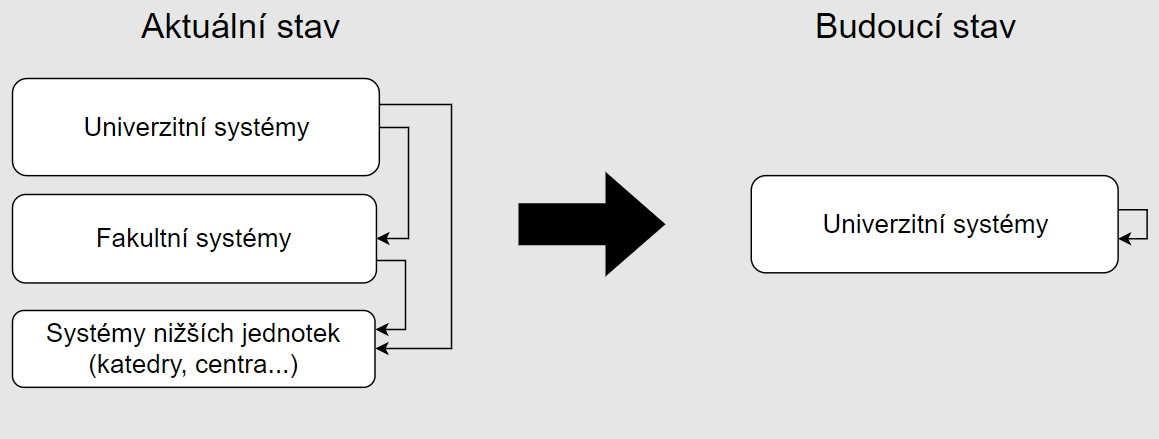
\includegraphics[width=\linewidth]{img/ctu-infrastructure.png}
	\caption{Schematické zobrazení informační infrastruktury ČVUT a komunikace systémů (zdroj autor)}
	\label{fig:ctu-infrastructure}
\end{figure}
Z dlouhodobého hlediska je tendencí strukturu zjednodušovat, tedy přesouvat kompetenci správy systémů na vyšší úrovně v hierarchii. Například tedy zamezit vzniku katederním systémům a místo toho zakládat centrální fakultní systémy. Toto řešení má výhody při změnách (ať už metodických, tak implementačních). Na druhou stranu může být toto řešení dosti personálně náročné, jelikož by se univerzita musela v budoucnu starat o všechny systémy. Zároveň by se tímto způsobem však měla spousta systémů eliminovat. Přechod na takové vnitřní uspořádání nelze provést skokově. Vhodnější jsou pozvolné změny, které však trvají velmi dlouho. \par
\noindent O jednotlivých systémech, které budou relevantní v kontextu této práce, se zmíníme v následujících kapitolách.





% a.	Úvod o fakultě, co je to za organizaci, jak zachází se znalostmi, jak je na tom informační infrastruktura.... – AS-IS
% případně navázat i TO-BE stavem - přínos pro školu
    \chapter{Analýza datových zdrojů} \label{chap:data-sources-analysis}
V následující kapitole shrneme výstupy analýzy datových zdrojů pro FEL ČVUT, která je jedním z cílů této části práce. Obecně jsme datové zdroje řešili v kapitole č. \ref{chap:sources}, nyní na tuto kapitolu navážeme a budeme řešit konkrétní příklady. Zdroje budeme dále kategorizovat do různých skupin. Důležité je zmínit, že v této kapitole nepopíšeme přesný způsob využití jednotlivých zdrojů. Spíše popíšeme, v jaké formě jsou data dostupná a jak by mohla být užitečná.\par
\section{Kategorizace datových zdrojů}
Datové zdroje můžeme rozdělit dle různých kritérií. V této sekci shrneme kategorie, které budeme používat v naší práci.
\paragraph{Dle typu obsahu na:}
\begin{itemize}
    \item Osoby a pracoviště
    \item Znalosti
\end{itemize}
\paragraph{Dle typu znalosti (viz kapitola č. \ref{chap:sources}) na:}
\begin{itemize}
    \item Znalostní báze
    \item Osobní znalosti
    \item Obojí
\end{itemize}
\paragraph{Dle příslušnosti datového zdroje na:}
\begin{itemize}
    \item Externí zdroj (případně globální)
    \item Interní zdroj pro danou organizaci - v našem případě pro ČVUT FEL
\end{itemize}

\section{Datové zdroje ČVUT}
% [TODO: obecně ještě zhodnotit ty zdroje, co se týká toho, jak jsou vhodné pro nás]
\subsection{Osoby a pracoviště}
% Co se týká dat o osobách, je důležité zmínit, že můžeme získávat buď jen data veřejně dostupná, nebo je nutné sbírat souhlasy od dotyčných osob.\par
\begin{table}[H]
\begin{ctucolortab}
% \begin{tabular}{|l|l|m{3cm}|l|m{2,75cm}|}
\begin{tabularx}{0.95\linewidth}{l|X|X|X}
\bfseries  & \bfseries Forma dat & \bfseries Dostupnost dat  & \bfseries Správce\\\hline 
    % \hline
    %  & Forma dat & Dostupnost dat & Aktualizováno & Správce \\ \hline
    \textbf{Usermap} & REST API (JSON) & veřejná data o zaměstnancích, po domluvě dostupná & ČVUT spravuje systém, FIT spravuje API \\\hline
    \textbf{UDB} & LDAP (LDIF) & veřejná data o zaměstnancích, po domluvě dostupná & FEL \\
\end{tabularx}
\end{ctucolortab}
	\caption{Tabulka dostupných zdrojů osob a pracovišť FEL (zdroj autor)}
	\label{tab:data-sources-people-fel}
\end{table}

\subsubsection{Usermap}
Usermap je centrální systém ČVUT pro správu identit. Jsou zde uloženy informace o osobách, organizační struktuře, pracovištích a jiné. Databáze Usermap má dvě části - LDAP databáze a přidružená relační databáze \cite{usermap-db}. Databáze Usermap je spravována jednotně na úrovni celé univerzity.\par
\begin{figure}[htbp!]
	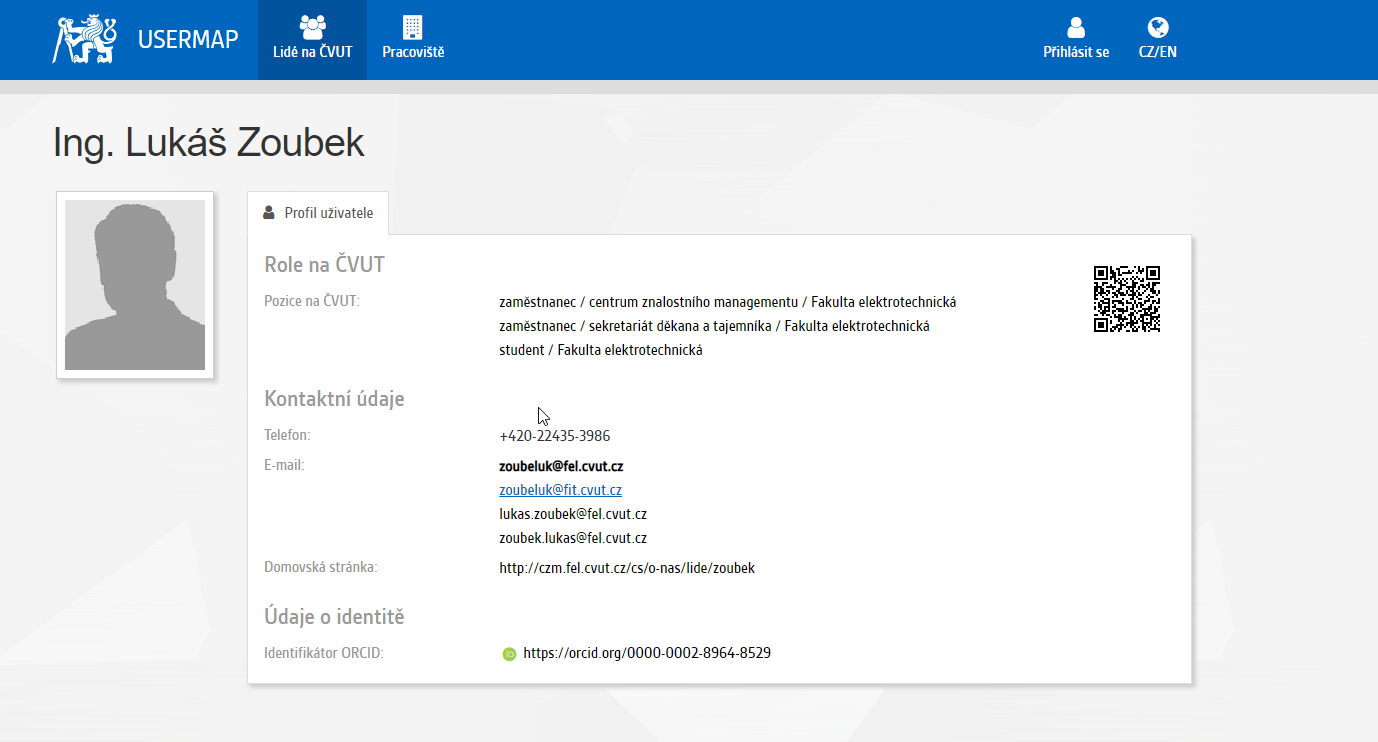
\includegraphics[width=\linewidth]{img/usermap.png}
	\caption{Webové rozhraní systému usermap (Dostupné z:  \url{https://usermap.cvut.cz/search})}
	\label{fig:usermap}
\end{figure}
\noindent REST rozhraní (\textit{Usermap API}) k této databázi je oproti tomu spravováno FIT ČVUT, konkrétně Ing. Jakubem Jirůtkou.
\begin{quote}
 \textit{Usermap API (pracovní název) je agregátor údajů o identitách lidí na ČVUT, který vyvíjíme na FIT. Poskytuje základní informace o osobě jako je jméno, uživatelské jméno, emailové adresy, telefony, … a tzv. byznys role (z IDM). Dále obsahuje informace o organizačních jednotkách ČVUT a místnostech (vč. adresy).} \cite{usermap-api}
\end{quote}
Identifikace v rámci tohoto zdroje probíhá pomocí uid, uživatelského jména v rámci ČVUT. Ve webovém rozhraní aplikace usermap lze též získat ORCID dané osoby - jednoznačný identifikátor vědeckých a dalších akademických autorů\cite{orcid}.
\subsubsection{UDB}
Narozdíl od systému usermap systém UDB je spravován fakultou FEL. Typy obsahu jsou ve své podstatě totožné, nicméně v UDB se nacházejí některá data navíc (fakultního charakteru). K systému neexistuje žádná veřejně dostupná dokumentace.
\subsection{Znalosti}
Již v kapitole č. \ref{chap:sources} jsme zmínili, že jeden fyzický zdroj může být jak zdrojem osobních znalostí, tak zdrojem znalostní báze. V této kapitole jsme se pokusili tyto dvě kategorie od sebe oddělit, nicméně se dá předpokládat, že zdroj nemusí mít vždy jedno diskrétní využití.
\subsubsection{Osobní znalosti}
\begin{table}[h!]
\begin{ctucolortab}
\begin{tabularx}{0.95\linewidth}{l|X|X|X}
\bfseries  & \bfseries Forma dat & \bfseries Dostupnost dat  & \bfseries Správce\\\hline 
    \textbf{V3S} & REST API (XML) & veřejná část & ČVUT spravuje systém, FIT spravuje API \\ \hline
    \textbf{KOS} & REST API (XML) & veřejná část & ČVUT spravuje systém, FIT spravuje API
\end{tabularx}
\end{ctucolortab}
	\caption{Tabulka dostupných zdrojů osobních znalostí na ČVUT (zdroj autor)}
	\label{tab:data-sources-people-fel}
\end{table}
\paragraph{Systém V3S:} V naší práci, jak jsme zmínili již v úvodu, se zabýváme více formálními zdroji znalostí (např. vědecké články, patenty). Předpokládáme, že systém V3S je pro data tohoto typu klíčový. Pokud bychom řešení opřeli o tento systém, množinu vyhledávaných bychom omezili na ty, kteří jsou vědecky aktivní. Má tedy smysl se zabývat i ostatními zdroji.\par
Aplikace V3S obsahuje záznamy o veškeré vědecké činnosti na univerzitě. Záznamy obsahují metadata o publikovaných článcích, autorech a dalších souvisejících entitách. Plné texty některých článků jsou k dispozici v digitální knihovně ČVUT (Dspace - https://dspace.cvut.cz/\url{https://dspace.cvut.cz/}). Nejedná se však o všechny články, ne všechny může ČVUT takto ukládat a poskytovat.\par
\noindent REST rozhraní \textit{V3S API} k této databázi je spravováno FIT ČVUT, konkrétně Ing. Jakubem Jirůtkou.\par
\paragraph{KOS (Komponenta studia):} KOS je centrálním informačním systémem pro podporu výuky na ČVUT. Studenti ČVUT přistupují do tohoto systému pomocí webového rozhraní, které obsahuje pouze zlomek dat, které jsou ve skutečnosti v systému k dispozici (v jeho databázi). REST rozhraní \textit{KOS API} k této databázi je správováno FIT ČVUT, konkrétně Ing. Jakubem Jirůtkou.\par
 KOS by mohl být potenciálně zdrojem obsahu jako: studované a vyučované předměty, vedené a nabízené závěrečné práce.\par
\paragraph{Ostatní:} Pracovníci FEL ČVUT mohou sami sloužit jako zdroj jejich znalostí - jejich životopisy, osobní stránky a jiné. Tyto zdroje typicky postrádají jakoukoliv jednotnou strukturu či rozhraní, jsou tedy špatně strojově zpracovatelné.
 \begin{figure}[htbp!]
	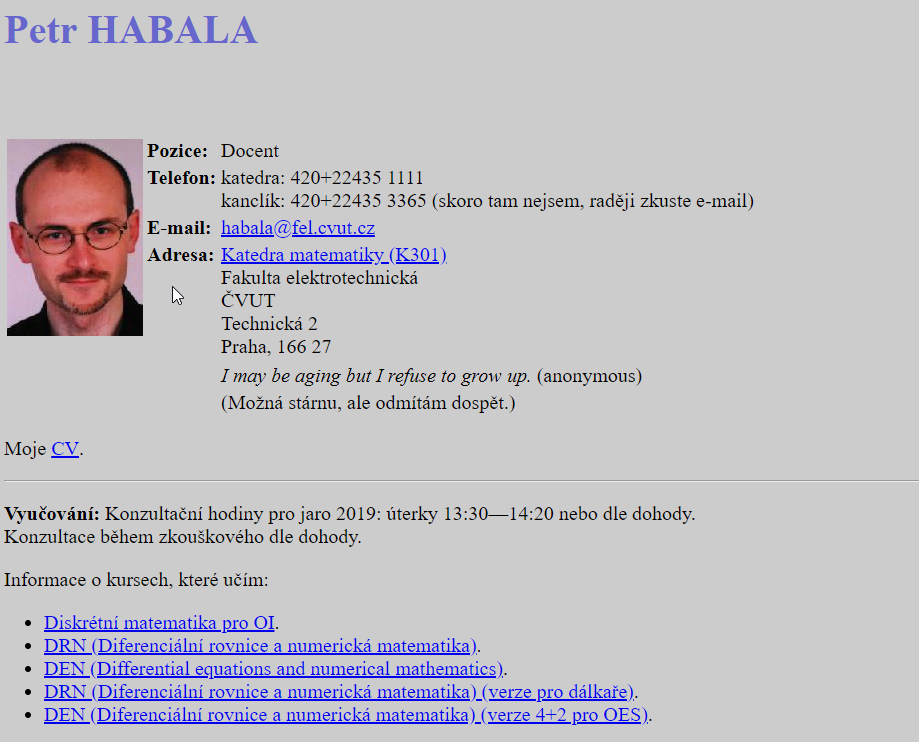
\includegraphics[width=\linewidth]{img/personal-pages.png}
	\caption{Webové stránky pracovníka katedry matematiky, docenta Habaly (Dostupné z:  \url{https://math.feld.cvut.cz/habala/indexc.htm})}
	\label{fig:personal-pages}
\end{figure}
 Při rešerši možných zdrojů jsme narazili ještě na systém DNEP (databáze nabídek, expertů a přístrojů), který nejspíše spravuje ČVUT. Systém obsahuje expertů pouze 93 (zjištěno z aplikace), na základě tohoto faktu jsme konstatovali, že není dále aktualizován a používán.

\subsubsection{Znalostní báze}
Potenciálně využitelným zdrojem znalostní báze přímo na ČVUT by mohl být systém V3S potažmo digitální knihovna DSpace. Data v těchto zdrojích (hlavně texty) by se po anotaci \cite{semantic-annotation} mohla použít při plnění ontologií, slovníků a jiných.\par 
Sémantická anotace textu je jednou z možných technik pro obohacování textu o význam, což je při tvorbě znalostní báze dosti klíčové. Sémantická anotace textu není triviální činnost, ruční provedení může trvat velmi dlouho a semi-automatické či automatické necháme na budoucí práci (zabývají se jí například nástroje jako je Tagtog - dostupné z: \url{https://www.tagtog.net/}, nebo LightTag dostupné z: \url{https://www.lighttag.io/}).

\section{Externí (globální) datové zdroje}
Při získávání informací o osobách a pracovištích jsme odkázáni na interní zdroje, externí zdroje můžeme použít pro znalosti. 
\subsection{Znalosti}
\subsubsection{Osobní znalosti}
Systém V3S považujeme za nejdůležitější a nejobjektivnější zdroj znalostí vědeckých pracovníků FEL. Další podobné zdroje jsou zmíněny v této sekci, jedná se však již o systémy, které nejsou ve správě fakulty/univerzity.
%  Jak jsme již zmínili v úvodu této sekce a v sekci zabývající se systémem V3S, nejkvalitnější data týkající se znalostí jsou pro nás výstupy vědecké činnosti. 
 %Dalšími potenciálními zdroji by pochopitelně mohli být některé veřejně dostupné informace např. sociální sítě aj., ty jsme však v této práci vynechali, soustředíme se více na oficiální zdroje. 
\begin{table}[h!]
\begin{ctucolortab}
\begin{tabularx}{0.95\linewidth}{X|p{5cm}|X}
\bfseries  & \bfseries Forma dat &  \bfseries Správce\\\hline 
    \textbf{Scholar, google patenty} & oficiální API chybí & Google\\ \hline
    \textbf{Scopus} & REST API (různé formáty) & Elsevier B.V. \\ \hline
    \textbf{Science Direct} & REST API (různé formáty, též fulltext search) & Elsevier B.V.\\ \hline
    \textbf{Springer} & REST API (různé formáty & Springer Nature \\ \hline
    \textbf{IEEE explore} & REST API (různé formáty) & IEEE \\ \hline
    \textbf{Web of Science} & REST API (různé formáty) & Clarivate Analytics \\ \hline
    \textbf{IS výzkumu, experimentálního vývoje a inovací} & API \cite{rvvi} & Úřad vlády České republiky \\ \hline
\end{tabularx}
\end{ctucolortab}
	\caption{Tabulka některých veřejně dostupných zdrojů osobních znalostní (zdroj autor)}
	\label{tab:data-sources-public}
\end{table}

 V rámci veřejných rozhraní je třeba vyřešit identifikaci osob z FEL ČVUT. Vzhledem ke zdrojům které máme k dispozici, se zaměřujeme nejvíce na vědecky aktivní část FEL ČVUT. Existují různé způsoby, jak identifikovat vědce či vědkyně.\par
 \paragraph{Příklady identifikátorů:}
 \begin{itemize}
     \item ORCID - Open Research and Contributor ID (neproprietární)
     \item RID - ResearcherID (proprietární Web of Science)
     \item Scopus Author ID (proprietární Scopus)
 \end{itemize}

\subsubsection{Znalostní báze}
% [TODO: možná zmínit, co od takového zdroje očekáváme]
Je důležité zmínit, že množství dostupných strukturovaných dat, které lze považovat za znalosti, je omezené. Existující datové množiny jsou mezi sebou provázány. Nejčastějšími primárními zdroji jsou Wordnet a Wikipedia (případně její strojově lépe čitelná verze DBPedia). Navazující projekty s těmito zdroji pracují a přidávají další, často užitečné, informace (aktivní přispívání znalostí však často neprobíhá).\par
\noindent Na základě tohoto kritéria datové zdroje rozdělíme do dvou skupin:
\begin{itemize}
    \item Primární zdroje - DBPedia, Wordnet
    \item Agregátory a procesory znalostí - ConceptNet, Yago, Datamuse, Twinword API, WordsAPI
\end{itemize}
% Uvádíme pouze příklady datových zdrojů znalostní báze. Další dostupné zdroje mohou být dostupné například u velkých poskytovatelů jako je Google (dostupné na: \url{https://console.cloud.google.com/apis}) aj.

\paragraph{DBpedia:}
DBpedia extrahuje informace z Wikipedie a následně data propojuje s ostatními získanými daty. Tímto způsobem vzniká jednotná znalostní báze \cite{db-pedia-article}. Tato znalostní báze je dostupná buď ve formě RDF s definovaným OWL schématem ke stažení, přes SPARQL rozhraní nebo též přes webové REST rozhraní \cite{db-pedia-web}. V roce 2014 měla DBpedia 3 miliardy RDF triplů. \cite{db-pedia-web}
\begin{figure}[htbp!]
	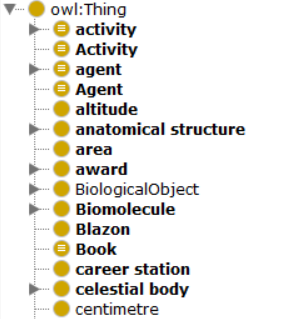
\includegraphics[width=0.45\linewidth]{img/db-pedia.png}
	\caption{Část ze schématu DBpedia v programu Protégé \url{https://protege.stanford.edu/} (zdroj autor)}
	\label{fig:dbpedia}
\end{figure}
\paragraph{WordNet:}
Dalším významným datovým setem je Wordnet. Jedná se o rozsáhlou lexikální databázi anglického jazyka. Slova jsou seskupována do množin synonym. Tyto množiny jsou později propojeny do sítí na základě významových a lexikálních vztahů. Wordnet neřeší slova pouze jako množinu znaků, orientuje se na jejich význam a pracuje například s podobností významu různých slov. \cite{princeton-wordnet} \par
\noindent Data jsou dostupná volně ke stažení, případně přes REST API \cite{princeton-wordnet}.
\paragraph{Agregátory a procesory:} \par
ConceptNet je volně dostupná sémantická síť čerpající mimo jiné z projektů DBpedia a Wordnet. Jedním ze zdrojů dat byla též komunita lidí, projekt Open Mind Common Sense. ConceptNet má API s výstupním formátem JSON-LD. \cite{ConceptNet} 
% [možná odcitovat ještě stránky, ten paper je odkazován na stránkách, ale nevím, co v něm je]
\par
Yago je rozsáhlá sémantická znalostní báze, která čerpá mimo jiné z Wikipedie a Wordnetu. Yago má více než 10 milionů entit. \cite{yago} Yago ontologie je k dispozici ke stažení, například ve formátu TURTLE. Software Yago je k dispozici ve formě zdrojového kódu též volně ke stažení.\cite{yago-web}\par
Dalšími datovými zdroji spadajícími do této kategorie mohou být například Datamuse \cite{datamuse}, Twinword API \cite{twinword} nebo Words API \cite{words-api}. Funkce, kterými disponují jsou typicky hledání slov s podobným významem, hledání slov souvisejících, hledání definic, lematizace (postup převádějící slova na základní gramatický tvar). \par
\section{Shrnutí}
V této kapitole jsme se zabývali rešerší datových zdrojů na FEL ČVUT, tím jsme navázali na kapitolu \ref{chap:sources}, kde jsme tuto problematiku řešili obecně.\par
Datové zdroje jsme rozdělili do kategorií a u každého jsme zmínili důležité parametry. Tím jsme naplnili jeden z cílů této práce.

% [TODO: obecný úvod - co je to za zdroje, co poskytují]


% \begin{table}[h!]
% \begin{tabular}{|m{3cm}|l|m{3cm}|l|m{2,75cm}|}
%     \hline
%     \cellcolor[HTML]{FFFFFF} & Forma dat & Správce \\ \hline
%     \textbf{CoceptNet} & oficiální API chybí & Google\\ \hline
%     \textbf{DBpedia} & REST API (různé formáty) & Elsevier B.V. \\ \hline
%     \textbf{Yago} & REST API (různé formáty, též fulltext search) & Elsevier B.V.\\ \hline
%     \textbf{WordNet} & REST API (různé formáty & Springer Nature \\ \hline
%     \textbf{Google data} & REST API (různé formáty) & IEEE \\ \hline
%     \textbf{Graphwords} & REST API (různé formáty) & Clarivate Analytics \\ \hline
%     \textbf{Datamuse} & API \cite{rvvi} & Úřad vlády České republiky \\ \hline
%     \textbf{Twinword} & API \cite{rvvi} & Úřad vlády České republiky \\ \hline
%     \textbf{Wordapi} & API \cite{rvvi} & Úřad vlády České republiky \\ \hline
% \end{tabular}
% 	\caption{Tabulka některých veřejně dostupných zdrojů znalostní báze (zdroj autor)}
% 	\label{tab:data-sources-public-knowledge.base}
% \end{table}


% %  - https://aleph.nkp.cz/F/DST1KFNIRM63S8U5SV5FJ9CF73L4H7PL9CR7Q4RUYBAKXG85BK-30094?func=file&file_name=find-b
% CoceptNet - http://conceptnet.io/
% DBpedia - https://wiki.dbpedia.org/
% Yago - https://datahub.io/collections/yago
% WordNet - https://wordnet.princeton.edu/ (případně jiné slovníky - Collins, https://onelook.com, Oxford, Wordnik, )
% google.com - translator
% https://graphwords.com/word#wood
% % https://en.wiktionary.org/wiki/deep_learning#English
% http://www.wiksearch.com/?s=buttock
% http://www.datamuse.com/api/
% https://www.twinword.com
% https://www.wordsapi.com


%  [Potenciálně do této kapitoly dodat tabulku s přehledným srovnáním aplikací, potenciálně jejich srovnání v rámci vlastností dobrých datových zdrojů pro ontologické zpracování]

 
 
 
 







%  \section{Datové zdroje dostupné pro ČVUT FEL}
%  Datové typy, které jsou potřeba pro tvorbu databáze znalostí jsou: \textit{Osoby, pracoviště a znalosti}. Tyto entity lze v každé organizaci získat různými způsoby. V kapitole o obecných datových zdrojích [TODO: odkaz] jsme konstatovali, že \textit{Osoby a pracoviště} jsme schopni získat poměrně přímočarým způsobem. \textit{Znalosti} jsou na rozdíl od těchto dvou entit velmi komplikovaným datovým typem. V sekci [TODO: odkaz], o reprezentaci dat, jsme rozebrali různé způsoby, jak znalosti reprezentovat. V závěru jsme se rozhodli, že nejvýhodnější bude použít reprezentaci pomocí ontologií. V dalších sekcích [TODO: sekce odkaz] jsme řešili, v jaké podobě jsou většinou data dostupná (XML, JSON) a do jaké podoby je chceme dostat (jakýkoliv typ serializace RDF - RDF XML, JSON LD, Turtle).\par


% \par
%  Důležité je brát v úvahu, že znalosti jsou velmi abstraktní pojem, i přesto že jsme si zvolili formu jejich reprezentace. V této sekci zmíníme i zdroje, které nejsou aktuálně uchopitelné pro přímou transformaci do ontologického schematu. Momentálně je takových zdrojů většina, protože FEL ČVUT neudržuje anotovaná dat na tak vysoké úrovni. Často tedy budeme zmiňovat zdroje, které momentálně nelze vzít, tak jak jsou, a přetransformovat do ontologického schematu.
%  \subsection{Znalosti vázané na osoby FEL ČVUT}
%  Takový datový zdroj musí znalost (v libovolné formě) poskytovat i s vlastníkem. Jinými slovy se jedná o zdroje, kde vlastník figuruje v libovolné spojitosti s entitou, kterou budeme považovat za znalost (resp. budeme počítat, že půjde vhodným definovaným způsobem transformovat na znalost). Zároveň musí takový zdroj vracet sílu znalosti v rámci daného datového zdroje (TODO: odkaz na data-processing), což je atribut vazby mezi znalostí a vlastníkem (TODO: odkaz na diagram, možná ještě nakreslit obrázek sem ve větším detailu, který shrnuje ten úvod celé té kapitoly).\par


%  -	Usermap
% o	Lidé a role, pracoviště
% o	https://kosapi.fit.cvut.cz/usermap/doc/rest-api-v1.html#
% o	Měl bych mít přístup ke všemu – read.

% -	https://udb.fel.cvut.cz/
% o	Po přihlášení!
% o	Vyhledávání dle username, jméno, příjmení
% o	Vyhledávání pracovišť
    \chapter{Návrh aplikace} \label{chap:app-design}
% Jedním z cílů této části práce je obecný návrh systému pro vyhledávání osob a pracovišť dle jejich kompetencí.
V následující kapitole rozebereme zevrubně návrh systému pro vyhledávání osob a pracovišť dle kompetencí. Budeme postupovat od nejobecnějšího (cíle a požadavky) ke konkrétnímu (případy užití, volba architektury). Stále se budeme pohybovat po technologicky nezávislé rovině, tu rozebereme až v následující kapitole při popisu prototypu. Stejně tak otázky reprezentace jsou na této rovině irelevantní, přestože ty jsme již rozhodli.
% Přestože jsme v první části této práce zmínili jako vhodnou reprezentaci znalostí ontologie, v této kapitole 
% Dokonce je na místě se v této kapitole odstínit i od dříve zmíněných ontologií, jelikož architektura aplikace by na takových věcech neměla být závislá.

% [TODO: Dekompozice problému budeme na to dbát při návrhu architektury pozdějšího systému - musíme být schopni nahradit moduly --> to by se hodilo na to navázat v úvodu té sekce Architektura]

\section{Podnět vzniku aplikace} %(to by mělo být zjevné již od začátku práce!)
Idea této aplikace pro vyhledávání osob dle kompetencí vznikla na FEL ČVUT, konkrétně u pana Ing. Martina Klímy, Ph.D.\par
Pan Klíma měl představu, že by měla na webových stránkách FEL vzniknout sekce, kde by třetí strany, konkrétně průmysloví partneři, mohli vyhledávat osoby dle jejich kompetencí. Partneři by později mohli kontaktovat daného člověka případně jeho vedoucího pracovníka, pokud by měli zájem s ním více spolupracovat. Tímto způsobem by tedy fakulta nabízela pracovníky a jejich kompetence širší veřejnosti, samozřejmě s jejich souhlasem.\par
První práce, která vznikla na toto téma je bakalářská práce Romana Kuchára z roku 2016. Pan Kuchár problematiku řešil poměrně přímočaře, způsobem, který pan Klíma popsal. \cite{kuchar} Po analýze kódu lze postup shrnout do následujících kroků:
\begin{enumerate}
    \item \textbf{Uživatel} zadá klíčové slovo tzv. expertise
    \item \textbf{Systém} nalezne výskyt tohoto slova v článcích v systému V3S (v titulu, klíčových slovech či abstraktu)
    \item \textbf{Systém} na základě hodnocení nalezených publikací (tzv. rivs) ohodnotí nalezené autory, přitom vezme v úvahu i míru jejich participace
    \item \textbf{Systém} vrátí seznam nalezených autorů seřazený dle jejich vypočteného hodnocení
\end{enumerate}
Řešení pana Kuchára v kontextu naší práce spadá pod varianty bez znalostní báze a bez práce se znalostmi vůbec (což nemusí být nutně špatně). V kapitole č. \ref{future} se zmíníme o řešeních tohoto typu.\par
Cílem této práce je celou problematiku prověřit zevrubněji (jak je vidět z první části této práce). Při návrhu aplikace budeme vycházet z požadavků/cílů, které definoval v úvodu pan Klíma a z požadavků, které jsme při této práci dále identifikovali.\par
Existuje mnoho dalších možností, jak vzniklou aplikaci obohatit o další užitečné funkce. V této práci však budeme pracovat se základními požadavky, pomocí kterých budeme tvořit jádro aplikace.
\section{Vymezení této práce}
\subsection{Rozsah řešené problematiky}
Na úvod upřesníme, čím se budeme v následujících sekcích zabývat. Celou problematiku vyhledávání osob a pracovišť dle jejich kompetencí, která vyplývá z pokynů k vypracování této práce, jsme v předchozí části práce zúžili na vyhledávání osob a pracovišť dle znalostí (viz kapitola \ref{chap:data_representation}). Pro účely následujících kapitol zúžíme celý problém pouze na vyhledávání osob dle znalostí.\par
Primárním důvodem je, že z definice kompetence pracoviště (kapitola \ref{sec:terms}) vyplývá, že je složena z kompetencí osob. Vyřešíme-li tedy problém vyhledávání osob dle kompetencí, stěžejní část problému vyhledávání pracovišť dle kompetencí vyřešíme též. Se znalostmi je to v tomto kontextu stejné jako s kompetencemi.\par
% Sekundárním důvodem je rozsah této práce, který je dostačující i bez dalšího případu užití.
\subsection{Rozsah navrženého systému}
Jak jsme zmínili výše, v následující kapitole rozebereme návrh aplikace pro vyhledávání dle kompetencí. Důležité je zmínit, že navrhneme celý systém až na část, která se zabývá transformací dat. Transformací dat, kterou jsme popsali v předchozí kapitole (č. \ref{chap:data-sources-analysis}), se vzhledem k rozsahu problematiky zabývat nebudeme. Zmíníme jí však v kapitole budoucí práce (č. \ref{future}), jelikož je to problematika, která musí být před nasazením navrženého systému vyřešena - bez dat jej nelze využívat.\par
\subsection{Rozsah implementovaného prototypu}
V následující kapitole (č. \ref{chap:implementation}) se budeme zabývat prototypem, který jsme v rámci naší práce implementovali. Účelem implementační části této práce je dokázat, že řešení navržené v této kapitole je možné použít a že skutečně může po dalších rozšířeních fungovat v praxi. Nejedná se tedy o kompletní implementovaný systém. V úvodu příští kapitoly zmíníme konkrétně rozsah obou částí prototypu.

% V předchozí kapitole (\ref{chap:data-sources-analysis}) jsme rozebrali datové zdroje osob, pracovišť a znalostí dostupné na FEL ČVUT. V rámci návrhu aplikace
% V následující kapitole se budeme
% V rámci této práce na tuto část již nenavážeme řešením transformace dat do ontologií a tak dále. To je velmi komplikovaná problematika, vhodná pro další zkoumání, v rámci další práce. V této práci budeme pro další kapitoly předpokládat, že data máme připraveny ve zvolené struktuře.
% Navrhneme kompletní systém, implementujeme prototyp...
\section{Požadavky}
\subsection{Základní business požadavek}
Základní business požadavek, který naše aplikace musí splnit je: \textit{Umožnit třetím stranám fakulty (firmám, výzkumným centrům a jiným) vyhledávát pracovníky FEL ČVUT dle jejich kompetencí, s jejich svolením.}
\subsection{FURPS+ analýza} \label{furps}
\subsubsection{Funkce}
\begin{itemize}
    \item Vyhledat seznam pracovníků FEL seřazených dle jejich vypočtené síly znalosti na základě zadaného klíčového slova (libovolného nebo zvoleného z definované množiny slov)
\end{itemize}
% dobrovolné požadavky (pro lepší práci s API, další možnosti)
% - CRUD nad entitami - osoby, znalosti, pracoviště
% - pro definovaného člověka nalézt jeho znalost v definovaném odvětví
% - ...
\subsubsection{Použití}
\begin{itemize}
    \item Část aplikace, do které bude přistupovat koncový uživatel, musí být dohledatelná pomocí běžných vyhledávačů dle klíčových slov (minimálně google a bing)
    \item Část aplikace, do které bude přistupovat koncový uživatel, musí být jednoduchá k použití - očekávají se uživatelé, kteří jsou gramotní při běžné práci s počítačem (textové procesory, práce s prohlížečem a webovými formuláři)
    \item Koncový uživatel aplikace musí mít k dispozici příručku (nejlépe interaktivní formou přímo v rozhraní)
    \item Aplikace musí být dostupná bez přihlášení, login se toleruje jen pro případná speciální administrátorská práva
    \item API musí být kompletně zdokumentováno pro budoucí použití jinými programátory
\end{itemize}
\subsubsection{Spolehlivost a výkon}
Aplikace nemá žádná zvláštní omezení na spolehlivost a výkon. Předpokládá se spolehlivost na úrovni ostatních nekritických aplikací univerzity - 98\%. Aplikace nemá speciální požadavky na výkon.
\subsubsection{Údržba}
\begin{itemize}
    \item Použitá technologie musí být kompatibilní s budoucím správcem aplikace (FEL)
    \item Aplikace bude koncipována jako webová, ne nativní
\end{itemize}
\subsubsection{Bezpečnost}
Data, která budou dostupná z aplikace, mohou být pouze data veřejně dostupná.
% data o zaměstnancích, jelikož budou k dispozici bez přihlášení. V opačném případě musí aplikace umožnit sbírání souhlasů s využitím osobních údajů.
\subsubsection{Implementace}
Architektura aplikace musí být modulární. Celý problém vyhledávání osob dle kompetencí, reprezentace znalostí a vše okolo má velmi mnoho možných přístupů k řešení. Architektura aplikace musí umožňovat jednoduchou výměnu jednotlivých modulů za jiné implementace.
\subsection{Případy užití}
% Případů užití navrhované aplikace není mnoho, na druhou stranu je poměrně komplikované je realizovat. Konkrétně hlavní případ užití aplikace (UC1 - Vyhledat osoby na FEL dle kompetencí) a jeho část, kdy systém musí vyhledat znalost a osoby, je v podstatě jádrem celé této práce.\par
\subsubsection{Aktéři}
Aplikace bude ze své podstaty otevřena široké veřejnosti. Hlavním uživatelem tedy bude \textit{nepřihlášený uživatel}.
\subsubsection{UC1 - Vyhledat osoby na FEL dle kompetencí} \label{UC1}
\paragraph{Scénář:}
\begin{enumerate}
    \item \textbf{Uživatel} zadá klíčové slovo (libovolné nebo vybrané z definované množiny slov)
    \item \textbf{Systém} nalezne na základě zadaného klíčového slova kompetenci (reprezentovanou libovolným způsobem) a osoby, které se k ní vztahují. Následně \textbf{systém} vypočítá/vyhledá sílu kompetence pro každou nalezenou osobu. Nakonec tento seřazený seznam osob vrátí uživateli. Neexistuje-li žádná osoba s touto kompetencí, systém vrátí uživateli prázdný seznam. 
\end{enumerate}
Seznam vrácený uživateli může být parametrizován pomocí offset a limit. \textbf{Limit} určuje počet výsledků, který má být vrácen. \textbf{Offset} potom určuje pořadové číslo prvního řádku z výsledku, který má být uživateli vrácen.
\subsection{Wireframy}
\subsubsection{W-UC1 - Vyhledat osoby na FEL dle kompetencí}
\begin{figure}[htbp!]
	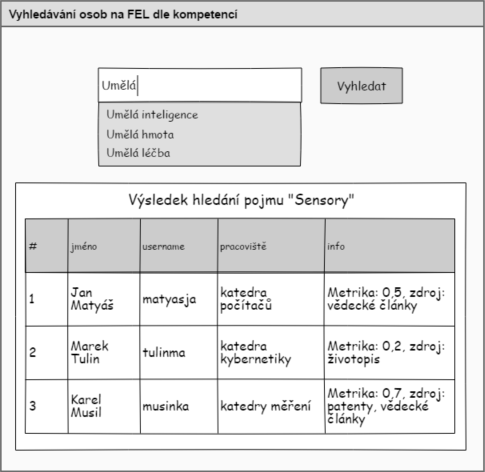
\includegraphics[width=0.9\linewidth]{img/W-UC1.png}
	\caption{Obrázek k W-UC1 (zdroj autor)}
	\label{fig:w-uc1}
\end{figure}
 \noindent \textbf{Vyhledávací pole} - zajišťuje uživatelský vstup, může být implementováno jako prosté textové pole s omezením na délku, či jako výběr s možností vyhledání\par
\paragraph{Tabulka s výsledkem obsahuje sloupce:}
\begin{itemize}
    \item Jméno - celé jméno osoby včetně titulů
    \item Username - username v rámci FEL ČVUT (slouží též jako email, po přidání domény)
    \item Pracoviště - název a kód pracoviště
    \item Info - libovolné informace, relevantní pro podložení vyhledaných informací a podobně
\end{itemize}

\section{Architektura aplikace}
Zkoumaný problém není složitý počtem funkcí, ale náročností jednotlivých celků. Tato náročnost se dosti odráží na architektuře celé aplikace. Aplikace může být integrována s různými typy úložišť a modularita musí zajistit jednoduché nahrazování jednotlivých částí (vyplývá z FURPS+ analýzy (\ref{furps})).
\subsection{Klient, Server}
Infrastruktura FEL ČVUT sestává primárně z webových aplikací. Tato platforma bude dodržena i v našem případě - viz FURPS+ (\ref{furps}).\par
Hlavní část aplikace je koncipována jako server s definovaným rozhraním, skrz které budou dostupné výše zmíněné případy užití. S rozhraním bude komunikováno pomocí HTTP protokolu. V této době jsou nejpoužívanějšími komunikačními přístupy: REST \cite{REST} a GraphQL \cite{GRAPHQL}, volba záleží na konkrétní realizaci.\par
Součástí této práce bude i klientská aplikace, na které demonstrujeme průběh komunikace se serverovou částí aplikace.
\subsection{Architektura}
Slovo architektura se v dnešní době používá v nesčetně významech. V praxi to často jde tak daleko, že již není ani zjevné, co má řečník opravdu na mysli.\par
Jak píše Martin Fowler, i když cynicky, ve své knize \textit{Patterns of Enterprise Application Architecture}, slovo architektura se používá, když lidé chtějí upozornit na něco, co je opravdu důležité. \cite{fowler-patterns}\par
Fowler poukazuje na to, že architektura je ve své podstatě rozpad systému na části a následné nastavení pravidel komunikace mezi těmito částmi. Možných architektonických vzorů je nespočet a klíčovým parametrem je nejčastěji dispozice ke změnám. Jinými slovy je klíčové, jestli se daná část aplikace bude v průběhu času měnit a jestli je tomu vybraná architektura dobře přizpůsobená. \cite{fowler-patterns}\par
V jedné aplikaci může být použito více architektonických vzorů \cite{fowler-patterns}. Dá se říct, že v tomto případě funguje přísloví \textit{účel světí prostředky}, pokud tedy daný vzor v dané situaci funguje správně, byl použit správně. Neexistuje samozřejmě jen jedno možné řešení, obzvlášť vezmeme-li v úvahu, jak rychle se technologie vyvíjí.\par
Architektura je subjektivní a je vždy závislá na systému i vývojovém týmu, který daný systém vyvíjí. \cite{fowler-patterns} Motivací, proč řešit architekturu, je nejčastěji potřeba vyhnout se pozdějším změnám, které jsou často časově náročné až likvidační.
\subsection{Výběr architektury}
Než přistoupíme k architektuře, která se nejvíce hodí pro náš systém, musíme shrnout úkoly, které aplikace bude plnit a data, která bude zpracovávat.
\paragraph{Data:}
\begin{itemize}
    \item Aplikační data - uživatelé aplikace, jejich práva, další data týkající se přídavných funkcí vyhledávače (historie hledání a podobně) 
    \item Zpracovávaná data - znalosti, osoby, pracoviště
\end{itemize}
\paragraph{Úkoly:}
\begin{itemize}
    \item Autorizace, autentizace, účty, cachování, další možnosti pro uživatele případně správce vyhledávače
    \item Poskytování všech druhů dat (CRUD operace)
    \item Uchovávání dat
    \item Zpracování znalostí, osob, pracovišť - agregace, reprezentace, operace při vyhledávání a jiné
    \item Získávání znalostí, osob, pracovišť
\end{itemize}
Ne všechny výše zmíněné úkony musí plnit první verze aplikace, dokonce nemusí existovat jen jediná aplikace, která celý problém bude řešit. Nicméně, jak jsme výše zmínili, je třeba počítat s budoucím nahrazováním jednotlivých částí a hledáním nových způsobů. Při volbě architektury tedy musíme počítat se všemi funkcemi, které nyní jsme schopni odhadnout.\par
Z FURPS+ analýzy (\ref{furps}) plynou zároveň požadavky na architekturu týkající se hlavně technologie a modularity vybraného řešení.\par
Systém není příliš složitý, co se týká počtu funkcí. Naproti tomu se však staví jeho komplexita vzhledem k integracím s jinými systémy (různé druhy databází, získávání dat z jiných API), která bude při volbě architektury klíčová. Z hlediska komplexity systému bychom tedy naší aplikaci nepovažovali za enterprise aplikaci v plném rozsahu, jak jí definuje Fowler ve své knize. Fowler píše, že enterprise aplikace obvykle zahrnují větší množství dat a paralelní přístup mnoha uživatelů  \cite{fowler-patterns}, což u naší aplikace nepředpokládáme. Naopak v ohledu integrace s jinými systémy se jedná o komplexní (enterprise) aplikaci a je třeba jí tímto způsobem navrhnout a spravovat.\par
Při tvorbě komplexnějších aplikací je jedním ze základních přístupů tzv. vrstvení (angl. layering) \cite{fowler-patterns}, rozhodli jsme se jej použít i v našem případě. Nejedná se o architektonický vzor, spíše o styl nebo přístup k tvorbě aplikací. Hlavním úkolem při tvoření vrstev je samozřejmě definice toho, za co každá vrstva zodpovídá \cite{fowler-patterns} a jak jsou nastavené závislosti mezi jednotlivými vrstvami.\par
Z počátku jsme zamýšleli použít vrstevnatou architekturi dle Browna (tabulka č. \ref{tab:brown}). 
\begin{table}[htbp!]
\begin{ctucolortab}
\begin{tabularx}{0.3\linewidth}{l}
                Prezentace \\ \hline
                Kontroler, mediator \\ \hline
                Doména \\ \hline
                Mapování \\ \hline
                Zdroj
\end{tabularx}
\end{ctucolortab}
	\caption{Tabulka vrstev architektury dle Browna (zdroj \cite{fowler-patterns}, přeložil autor)}
	\label{tab:brown}
\end{table}
Jak píše Fowler, v případě \textit{Brownovy architektury} můžeme vzít v úvahu další varianty. Můžeme vzít hlavní tři vrstvy a mezivrstvy dodávat v případě přílišné komplexity systému. \cite{fowler-patterns}\par
V takto vrstevnaté architektuře je komunikace mezi vrstvami typicky nastavena jedním směrem, tzn. že vrstvy mohou volat buď všechny vrstvy níže, nebo jen jednu o patro níž. 
% [obrázek beyond - classic layered architecture]
\par
\textit{Brownovu architekturu} můžeme klasifikovat jako klasickou vrstevnatou. Architektury tohoto typu mají jednu značnou nevýhodu, kterou je přílišné provázání celého systému (angl. coupling) s datovými zdroji. Datové zdroje (databáze, soubory, webové služby) jsou totiž typicky svázány přímo s aplikační logikou, přes definované mapování (viz předposlední vrstva v tabulce č. \ref{tab:brown}).\par
\noindent Na tento nedostatek poukázal ve své práci Jeffrey Palermo, který konkrétně zmiňuje:
\begin{quote}
    Kámen úrazu je v tomto případě fakt, že aplikace je postavená okolo dat a ostatní infrastruktury. Jelikož je aplikace takto provázána, tak pokud se změní přístup k datům, externí služba a podobně, musí se změnit i business logika aplikace. \cite{palermo}  (přeložil autor)
\end{quote}
% [TODO: obrázek od Jeffreyho]
Odstínění částí jako je databáze, které Palermo nazval infrastrukturou, je i pro nás velmi klíčové.
% Je tomu tak, protože není jasné, kolik způsobů bude třeba v budoucnu vyzkoušet, aby náš systém fungoval efektivně. V rámci této práce implementujeme jeden z možných způsobů.
\par
Palermo staví na místo toho jiný typ architektury. Architekturu, kterou nazval cibulová architektura (angl. Onion architecture). Tato architektura podle něj lépe pracuje s provázaností programu \cite{palermo} a tedy se i více hodí pro náš případ. Palermo ve své práci dodává, že se nejedná o zcela nový přístup, on je ale ten, kdo jej pojmenoval a propagoval.\par
\begin{figure}[htbp!]
	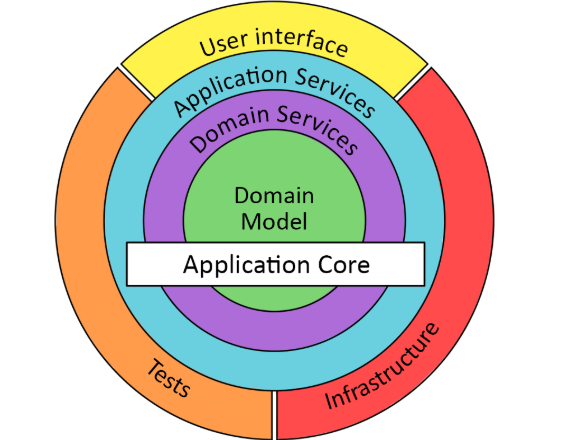
\includegraphics[width=0.7\linewidth]{img/onion.png}
	\caption{Cibulová architektura (zdroj \url{https://dzone.com/})}
% 	 articles/ onion-architecture-is-interesting
	\label{fig:onion}
\end{figure}
Cibulová architektura (obr. č. \ref{fig:onion}) se vyznačuje především tím, že infrastruktura je vždy považována za vnější vrstvu (na obrázku \textit{Tests, User interface a Infrastructure}). Ve středu je tzv. doménový model (na obrázku \textit{Domain Model}), který v podstatě reprezentuje entity reálného světa, které v systému používáme \cite{palermo} ve formě datových struktur (objektů). Doménový model je jediná část aplikace, která je závislá pouze sama na sobě. Na tuto vrstvu navazuje libovolný počet dalších vrstev. Obvykle zde bývá vrstva, která se zabývá manipulací s doménovým modelem - ukládání a získávání (na obrázku \textit{Domain Services}). Tato vrstva se zde vždy nachází ve formě rozhraní, implementace tohoto rozhraní je totiž až součást vyšší vrstvy infrastruktury. Nad těmito vrstvami se může nacházet další vrstva aplikační logiky, kde se již řeší business logika aplikace (na obrázku \textit{Application Services}). Okolo potom stojí infrastruktura (DB, soubory, webové služby), testy, uživatelské rozhraní. Závislosti mezi vrstvami jsou vždy koncipovány, tak aby jedna vrstva závisela pouze na vrstvách, které jsou v obrázku č. \ref{fig:onion} blíže ke středu. \cite{palermo}\par
Při použití této architektury bychom v našem případě mohli vyhovět požadavku na jednoduché provádění změn v infrastruktuře. To je totiž právě důvod, proč je cibulová architektura navržena tímto způsobem. Dle Palerma se totiž nejčastěji mění právě infrastruktura a tato architektura jí proto staví do vnější vrstvy, jejíž změny neovlivní doménu ani business logiku. \cite{palermo}\par
Cibulová architektura je tedy pro náš případ nejvhodnější, proto jsme se rozhodli pro jednu z variant této architektury - tzv. hexagonální architekturu.

\section{Hexagonální architektura - Porty a adaptéry}
Robert C. Martin (Uncle Bob) se ve své práci zmiňuje o několika architekturách, mezi nimi i cibulová a hexagonální, a shrnuje jejich společné znaky. Zmiňuje, že obě architektury mají stejný cíl, a to je oddělení zájmů (angl. separation of concerns), o tom se mimochodem zmiňuje i Jeffrey Palermo \cite{palermo}. Obě architektury tohoto dosahují rozdělením systému do vrstev a obě architektury oddělují business část aplikace od infrastruktury. \cite{uncle-bob} Systém, který staví na těchto principech je obvykle nezávislý na knihovnách, dobře testovatelný, architektonicky nezávislý na typu UI, typu databáze i na jiných externích systémech. \cite{uncle-bob}.\par
Hlavní myšlenku hexagonální architektury zformuloval Alistair Cockburn. Ve svém článku se odkazuje na stejné principy, které jsou zmíněny výše u Palerma. Nejvíce se opírá o myšlenku, že problematika poskytování dat a získávání dat je ve své podstatě totožná a není třeba jí řešit různými způsoby. Cockburn si všiml, že v jiných architekturách (například v Brownově zmíněné výše) je častým jevem, že při návrhu systému se s těmito dvěma problematikami zachází různým způsobem. Architektura se jinak nazývá též porty a adaptéry, protože ty se staly nástrojem, jak se vypořádat s poskytování a získáváním dat. \cite{cockburn}\par

\begin{itemize}
    \item \textbf{Porty} jsou vstupními body, které jádro aplikace poskytuje.\cite{bergen}
    \item \textbf{Adaptéry} slouží jako most mezi aplikací a službami, které jsou potřeba pro její chod. Vždy patří ke specifickému portu. \cite{bergen}
\end{itemize}
Přestože se architektura snaží řešit porty a adaptéry univerzálně, vzhledem k existenci různých aktérů v rámci systému, i porty a adaptéry se dále dělí. \cite{cockburn} \par
Aktéři jsou buď primární či sekundární. Primární aktér řídí aplikaci (typicky uživatel, ale například i test) - na obr. č. \ref{fig:hexagonal} \textit{Driver Side}. Sekundární aktér je řízen aplikací (typicky databáze, resp. databázový repositář) - na obr. č. \ref{fig:hexagonal} \textit{Driven Side}. \cite{cockburn} \cite{hexagonal-this}\par
% Porty a adaptéry se stejným způsobem dělí na primární a sekundární (na obrázku č. \ref{fig:dependency-hexagon} lze vidět, jak fungují v architektuře závislosti, které s dělením portů a adaptérů souvisí).
\begin{figure}[H]
	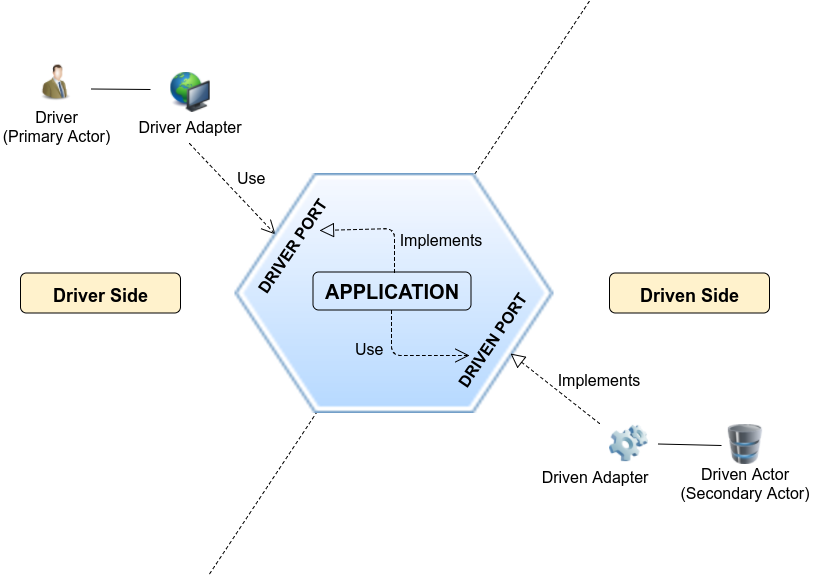
\includegraphics[width=\linewidth]{img/hexagonal-scheme.png}
	\caption{Hexagonální architektura (zdroj \cite{hexagonal-this})}
	\label{fig:hexagonal}
\end{figure}
\newpage
\begin{itemize}
    \item \textbf{Dělení portů}
        \begin{itemize}
            \item Primární - tvoří aplikační rozhraní nabízené aplikací (na obrázku č. \ref{fig:dependency-hexagon} API), jsou volány primárními adaptéry \cite{bergen} \cite{hexagonal-this}
            \item Sekundární - tvoří rozhraní vyžadované aplikací (na obrázku č. \ref{fig:dependency-hexagon} SPI), jsou volány jádrem aplikace \cite{bergen} \cite{hexagonal-this}
        \end{itemize}
    \item \textbf{Dělení adaptérů}
        \begin{itemize}
            \item Primární - volají primární porty, například testy aplikační logiky, kontroler pro komunikaci s UI (na obrázku č. \ref{fig:dependency-hexagon} Controller jako příklad) \cite{bergen}
            \item Sekundární - implementují sekundární porty, například databázové repozitáře, nebo mockovací knihovny (na obrázku č. \ref{fig:dependency-hexagon} Persistence jako příklad)\cite{bergen}
        \end{itemize}
\end{itemize}
Na obrázku č. \ref{fig:dependency-hexagon} je navíc dobře vidět, že celá aplikace je svázána doménovým modelem (na obrázku Domain Objects). \par
% Primárním adaptérům se někdy též říká řídící (angl. driver), naopak sekundárním se říká řízené (angl. driven), viz obr. č. \ref{fig:hexagonal} \cite{cockburn}.\par
\begin{figure}[H]
	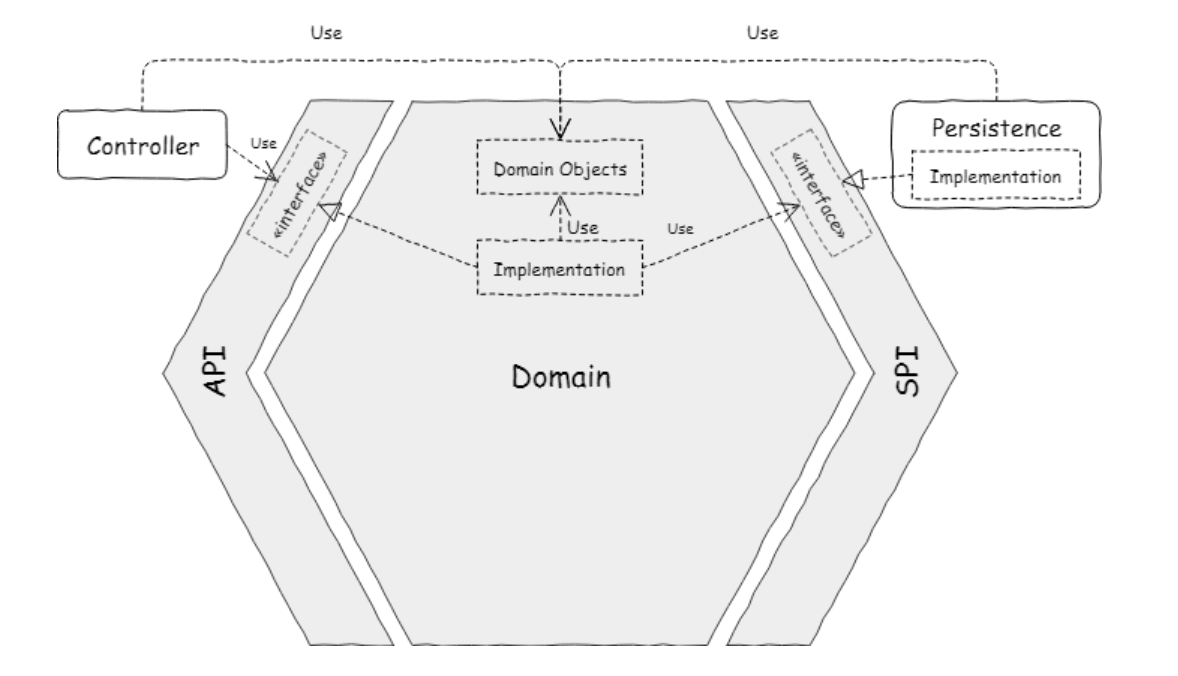
\includegraphics[width=\linewidth]{img/hexagon-dependency.png}
	\caption{Znázornění vzájemných závislostí v hexagonální architektuře (zdroj \cite{beyondxscratch})}
	\label{fig:dependency-hexagon}
\end{figure}
% Vzory typické
% zmínit se o dependency injection pattern - vyžaduje, jelikož se programuje striktně proti interfacům (bergen, campament) + můžu přidat obrázek patternů
Na závěr této sekce je důležité zdůraznit, že přes zmíněné kladné vlastnosti hexagonální architektury existují i záporné. Mezi ně patří především komplexita celého řešení, počet modulů zkrátka roste s počtem portů a adaptérů \cite{hexagonal-this}. Následně můžeme narazit díky komplexitě projektu (závislosti, moduly a podobně) na problémy s výkonem \cite{hexagonal-this} a s komplikovanou správou celého projektu. Jak jsme již zmínili zápory kompenzujeme klady, především dobrou připraveností na změny a testy.

\section{Hexagonální architektura pro náš případ}
V následující sekci shrneme, jak bude v našem případě použita hexagonální architektura. Představíme diagram komponent, doménový model a sekvenční diagramy. Důležité je, že se stále jedná o technologicky nezávislé modely, které popisují obecný návrh systému pro vyhledávání dle kompetencí.\par
\subsection{Komponenty}
Na diagramu komponent, který je součástí přílohy č. \ref{fig:component-model}, vidíme jednotlivé komponenty systému. Závislosti mezi nimi jsou navrženy tak, jak je tomu v hexagonální architektuře.
\subsubsection{Doména}
Jedná se o centrální část systému, která obsahuje doménový model, business logiku aplikace a porty. Na doméně závisí všechny ostatní komponenty aplikace.\par
\paragraph{Doménový model:} Tvoří jádro celého systému, v podstatě se v něm nachází základní entity reálného světa, které jsou v systému namodelovány. Součástí doménového modelu musí být pouze entity, jejich metody a vlastnosti, které nejsou závislé na konkrétním řešení.
Doménový model je součástí přílohy č. \ref{fig:domain-model} a má následující části:
\begin{itemize}
    \item Osoba - entita reprezentující osobu v dané organizaci (v našem případě FEL ČVUT)
    \item Pracoviště - entita reprezentující pracoviště v dané organizaci (v našem případě se jedná o katedry)
    \item Znalost - reprezentuje vazbu mezi osobou a konceptem, přidává jí navíc sílu a poznámku (napříkla jak daná znalost vznikla, resp. odkud jsme jí odvodili)
    \item Koncept - reprezentuje cokoliv, co může být poznáno osobou, jedná se o informace či atomické pojmenované skutečnosti (konkrétní reprezentace je podmíněna konkrétním řešením, domníváme se však, že bez konceptů se v nějaké podobě neobejde žádné řešení); je důležité nezaměňovat tento pojem s ontologickým konceptem, který reprezentuje ontologickou kategorii (viz \ref{ontologies})
    % , v kapitole č. \ref{sec:terms} je tento koncept označen jako \textit{předmět kompetence}
\end{itemize}
V diagramu jsou dále k vidění vazby mezi jednotlivými objekty i s popiskem. 
% Za zmínku stojí hlavně rekurzivní vazba konceptu. Tato vazba nastiňuje existenci sémantické vazby mezi koncepty. Není nutné, aby jí každé řešení muselo mít, v doméně jsme jí však obsáhli - tento druh modelování je v jistém smyslu omezený a není možné vždy striktně oddělit doménu od zbytku systému, který již není tak neměnný. [možná by to chtělo ještě promyslet]
\paragraph{Business logika:}
V této části aplikace jsou typicky k dispozici operace s entitami domény (CRUD) a implementované případy užití (hlavní aplikační logika). Business logika využívá SPI porty a její součástí je implementace API portů.\par
V našem případě se jedná převážně o logiku vyhledávání osob dle kompetencí a operace s tím spojené. V této části se používají SPI adaptéry, které poskytují další služby (například vyhledávání v DB).
\paragraph{Porty a adaptéry:}
Součástí domény jsou API a SPI porty ve formě rozhraní. Dle idey hexagonální architektury je součástí domény zároveň implementace rozhraní API portů.
\subsubsection{API}
V levé části diagramu komponent (\ref{fig:component-model}) je tzv. řídící část hexagonální architektury ve formě API adaptérů. Tyto adaptéry závisí na API portech implementovaných v doméně a volají jejich funkce. V naší aplikaci tyto adaptéry budou představovat typicky REST API případně GraphQL API. Předpokládáme, že tímto způsobem bude aplikace komunikovat s případnými příjemci (v diagramu komponent je takovýto klient také zobrazen). V obrázku lze též vidět, že předpokládáme logické oddělení Knowledge API, umožňující vyhledávání osob a Base API, které umožňuje základní aplikační případy užití (autentizace, případně další týkající se více správy aplikace, než samotného vyhledávání).

\subsubsection{SPI}
Na pravé straně diagramu (\ref{fig:component-model}) je vidět tzv. řízená část hexagonální architektury ve formě SPI adaptérů. Tato část je klíčová z pohledu odolnosti naší architektury vůči změnám použitého řešení. Bez ohledu na to, jaké konkrétní řešení pro vyhledávání dle kompetencí použijeme, domény se to dotkne jen minimálně. Naopak v této části SPI adaptérů, konkrétně u adaptérů zajišťujících samotné vyhledávání, předpokládáme změny. U uživatelských adaptérů (jak jsme je nazvali na obrázku \ref{fig:component-model}), které poskytují spíše aplikační logiku (například přihlašování), opět neočekáváme velké změny, přesto by to bylo možné. V diagramu jsme navrhli několik možných adaptérů, jedná se však pouze o příklady, v konkrétním případě záleží na zvoleném řešení. SPI Adaptéry zajišťují další komunikaci s případnými externími systémy (například databáze, API jiných systémů).\par
% Na diagramu komponent (\ref{fig:component-model}) jsou  na pravé straně zobrazeny databáze (DB), již však není vidět, že tyto databáze nemusí plnit samotná aplikace. U některých řešení se dá předpokládat, že další moduly stávající aplikace, nebo další drobné aplikace případně skripty budou databázi plnit. Plnění databází a celá logika získávání dat pro naše účely je velmi rozsáhlá a komplikovaná, v této práci se jí nezaobíráme. Pochopitelně tato problematika souvisí s transformací dat, kterou jsme zmínili v kapitole č. \ref{chap:processing}.
% [TODO možná moduly lépe namapovat na požadavky z úvodu)]
\subsection{Komunikační sekvence}
Součástí přílohy \ref{appendix:sequence} je diagram sekvencí, na kterém jsme se pokusili demonstrovat, jak bude probíhat komunikace mezi cílovým uživatelem naší aplikace a aplikací samotnou při volání UC1 (\ref{UC1}).
% [odkaz na UC, doplnit asi všude takovéto provázání mezi požadavky, UC apod.]. 
Zároveň je na něm k vidění, jak spolu komunikují jednotlivé komponenty aplikace.\par
Důležité je, že komunikace s aplikací může probíhat synchronně (\ref{fig:sequence-synchronous}) či asynchronně (\ref{fig:sequence-asynchronous}). To jinými slovy znamená, že výsledek hledání může koncový uživatel dostat ihned po dotazu, nebo mu bude navrácen identifikátor hledání a na jeho výsledek se zeptá později. Která varianta bude použita, záleží na zvoleném řešení.\par
% na tom, jak bude zvolené řešení časově náročné. Při delším zpracování není vhodné udržovat mezi oběma stranami synchronní připojení. Existují samozřejmě další faktory, které ovlivňují způsob této komunikace - použití vláken na straně serveru, asynchronní technologie (např. klientský Javascript, který nutně neblokuje webového klienta při další interakci) [TODO: podložit, nebo možná vyhodit, možná tu mluvím o různých věcech]. \par
% Je nezbytné dodat, že diagramy jsou pouze schématické, pro pochopení celého konceptu. Jsou v nich jistě části, které by se dali dotáhnout do větší úrovně detailu, to ale nebylo naším cílem. Naším cílem byla primárně srozumitelnost, jak tomu u diagramů bývá.
% Například SPI adaptérů (na obrázku [odkaz] tzv. adaptéry konkrétního řešení) může být několik a domény s každým z nich může komunikovat zvlášť. Ve většině případů lze vždy ještě nalézt výjimečné stavy (neúspěch při připojení do databáze apod.), které v diagramu pro zvýšení přehlednosti nejsou zohledněné. V neposlední řadě není zmíněno, že při asynchronním zpracování se uživatel může API zeptat na výsledek dříve než jej bude mít k dispozici. V takovém případě API vrátí zvoleným způsobem zprávu "vyhledávání stále probíhá".
\section{Shrnutí}
V této sekci jsme se zabývali návrhem systému pro vyhledávání osob dle jejich kompetencí. Začali jsme od cílů, požadavků a případů užití a pokračovali jsme až k detailnímu popisu zvolené architektury. V následující sekci na náš návrh navážeme popisem implementace prototypu.







% [diagram nasazení - technologicky nezávislý - nejspíš ne]

% - zamyslet se nad platnými pravidly, případně praktikovat reasoning
% - Vytvořit testovací data
% - Vložit do graphDB




% i.	Architektura aplikace – požadavek na modularitu a obecnost (nejdříve obecně, bez technologií
% \section{Hexagonální architektura - Porty a adaptéry}
% Architektura (udělat diagram komponent pro mé konkrétní použití)
% - Hexagonal (Port and Adapter)
% https://github.com/gshaw-pivotal/spring-hexagonal-example
% https://blog.octo.com/en/hexagonal-architecture-three-principles-and-an-implementation-example/
% - vložit obrázek z citovaného zdroje
    \chapter{Implementace} \label{chap:implementation}
V následující kapitole přistoupíme k popisu prototypu, který jsme v rámci této práce implementovali. Tím navážeme na předchozí kapitolu, ve které jsme řešili návrh systému.\par

\section{Rozsah implementovaného prototypu}
% Jedním z cílů této práce je implementace zvoleného řešení pro vyhledávání pracovníků dle kompetencí na FEL ČVUT.\par
\subsection{Server}
V serverové části prototypu je implementován základní případ užití, tedy UC-1 (\ref{UC1}). Prototyp obsahuje funkční zpracování hexagonální architektury, kterou jsme popsali v předchozí kapitole. Vertikální průřez aplikací je funkční, probíhá synchronní dotaz na funkční datové úložiště s testovacími daty, stejně jako je vidět na sekvenčním digramu (příloha \ref{fig:sequence-synchronous}).\par
% [TODO: nejsou zajištěny ani chybové stavy]
% Popis naimplementované části - neobsahuje AAA (vysvětlit proč), neobsahuje vyhledávání pracovišť (jedná se spíše o POC nikoliv o plnohodnotnou aplikaci), neřeším získávání dat, např. vůbec nejsou přítomny adaptéry aplikační logiky (AAA a jiné vychytávky jako je histrorie hledání apod.), je synchronní přesto, že zvolené řešení by možná vyžadovalo opak, API není kompletní
% Identifikovaná omezení
% - je třeba používat offset, limit, případně prefix, je poměrně pomalé vracet velké množství konceptů
\subsection{Klient}
Klientská část prototypu je přítomna pro demonstraci toho, že komunikace se serverovou částí probíhá a klient je schopný data zpracovávat. V tomto klientu lze vidět implementovanou obdobu W-UC1 (obr. č. \ref{fig:w-uc1}).

\section{Diagram komponent}
% [diagram i s vrstvami (?), možná digram nasazení ]
Diagram komponent konkrétního řešení je k vidění v příloze \ref{fig:component-graphDB}. Jelikož vychází z návrhu zmíněného v minulé kapitole, je obdobou obecného digramu komponent z přílohy \ref{fig:component-model}. V následujících sekcích rozebereme jednotlivé komponenty, technologie, které jsme pro jejich vývoj použili a zmíníme případné ukázky.

\section{Hlavní použité technologie}
V této sekci shrneme základní použité technologie, konkrétnější zástupce poté rozebereme u jednotlivých modulů. Soupis všech použitých technologií je poté připojen v příloze \ref{app:technology-list}.
\subsection{Programovací jazyk pro serverovou část}
Z požadavků specifikovaných v sekci \ref{furps} vyplývá, že použité technologie musí být kompatibilní s budoucím správcem aplikace, což by mělo být některé pracoviště FEL ČVUT. Druhým požadavkem je, aby aplikace byla koncipována jako webová (resp. jako webové rozhraní). V tomto kontextu přichází v úvahu jazyk JAVA, která má na FEL základnu. Variantou by mohlo být nespočet dalších jazyků, které umožňují vývoj webových enterprise aplikací. Jako rozhodující faktor, po požadavcích fakulty, v tomto ohledu vnímáme preference autora samotné aplikace. Jazyk JAVA vyhovuje implementačním dovednostem autora této práce, rozhodli jsme se tedy využít ten. \par
% [TODO: srovnání jazyků?]\par
V rámci jazyka JAVA je možné využít několik různých knihoven pro vývoj webových enterprise aplikací. Pro účely naší práce se mezi sebou příliš neliší.
\paragraph{Některé varianty knihoven:}
\begin{itemize}
    \item Implementace standardu JAVA EE
    \item JAVA Spring (případně jeho nadstavba Spring Boot)
\end{itemize}
V tomto ohledu bereme opět ohledy na preference autora. Zvolili jsme tedy, dnes velmi progresivní, variantu knihovny JAVA Spring, Spring Boot (dokumentace dostupná z: \url{https://spring.io/projects/spring-boot}). Hlavní výhodou Spring Boot je rychlost vývoje za podpory této knihovny a množství kódu, který musí koncový programátor napsat. Tato vlastnost se hodí, hlavně kvůli tomu, že nevyvíjeme kompletní aplikaci, ale prototyp.
% [TODO: srovnání knihoven]
\subsection{Programovací jazyk pro část klient}
Klientská část našeho prototypu bude se serverovou částí komunikovat pomocí REST rozhraní (popsáno níže). Jak jsme zmínili již v úvodu této sekce, klientská aplikace není příliš složitá a je přítomna jen pro demonstraci komunikace se serverem, proto výběr technologie nehraje velkou roli. Zvolili jsme tedy přístup bez jakékoliv další knihovny. Pro klientskou část jsme použili programovací jazyk Javascript, který řeší klientskou logiku, strukturu a vzhled poté řeší HTML a CSS.
\subsection{Databáze}
V kapitole č. \ref{chap:processing} jsme již zmínili příklady různých triple-store databází. Na databázi neklademe žádné speciální požadavky, pouze podporu RDF triplů. Námi zvolená databáze je volně dotupná verze GRAPH-DB (dostupná z: \url{http://graphdb.ontotext.com/}). GRAPH-DB mimojiné používá knihovnu RDF4J, která poskytuje rozhraní jazyku JAVA pro práci s RDF a dalšími přidruženými technologiemi (dokumentace dostupná z: \url{http://rdf4j.org/about/}).
% [TODO: argumentace proč, jsem jí zvolil]
\section{Struktura projektu}
Serverová část prototypu je členěna dle zvolené hexagonální architektury na jednotlivé moduly. V následujících sekcích se zaměříme na popis jednotlivých částí aplikace.
\begin{lstlisting}[caption= Schématicky zobrazená struktura projektu, captionpos=b]
knowledge_search/
|-- application/
    |-- config/
    |-- KnowledgeSearchApplication
|-- domain/
    |-- api/
    |-- logic/
    |-- model/
    |-- spi/
|-- gdb_solution/
    |-- adapters/
    |-- model/
    |-- dao/
|-- rest
    |-- controllers/
    |-- model/
\end{lstlisting} 

\section{Doména}
V diagramu komponent (\ref{fig:component-graphDB}) je doména ve střední části, ve struktuře projektu se nazývá \ctulst(none)!domain!. Doména má čtyři části \ctulst(none)!logic!, \ctulst(none)!model!, \ctulst(none)!spi! a \ctulst(none)!api!.\par
V části \ctulst(none)!logic! se nachází business logika celé aplikace. V nynější verzi se v této vrstvě volají spi repozitáře, složitější logika není přítomna.\par
\noindent Část \ctulst(none)!model! obsahuje doménový model aplikace ve formě rozhraní.
\begin{lstlisting}[language=JAVA, caption= Ukázka rozhraní jedné z entit v doménovém modelu, captionpos=b]
public interface Knowledge extends Identifiable{
    Double getMetric();
    String getInfo();
    <T extends Person> T getOwner();
    <T extends Concept> T getConcept();
}
\end{lstlisting}
Modul \ctulst(none)!spi! obsahuje repozitáře ve formě rozhraní, které později implementuje modul \ctulst(none)!gdb_solution!.
\begin{lstlisting}[language=JAVA, caption= Ukázka rozhraní SPI repozitáře, captionpos=b]
public interface PersonRepository {
    Collection<? extends Knowledge>
    searchPeopleByKnowledge(StringconceptId, int offset, int limit);
    Collection<? extends Person> getAllPersons();
}
\end{lstlisting}
Poslední modul domény je \ctulst(none)!api!, třídy v tomto modulu obsahují rozhraní a implementaci api portů. Tyto porty jsou později používány api adaptéry při volání aplikační logiky.
\section{Spouštěcí modul}
Modul \ctulst(none)!application! má v systému zásadní roli - spouštění a konfigurace aplikace. Spouštění aplikace zajišťuje vstupní bod, třída \ctulst(none)!KnowledgeSearchApplication!. Konfigurace obsahuje adresář \ctulst(none)!config/!. V tomto adresáři jsou definovány tzv. \textit{Spring Bean} třídy, které zajišťují předávání námi zvolené instance určitého objektu Spring IoC kontejneru. Kontejner s instancí dále v běhu aplikace nakládá a vrací jí tam, kde jí potřebujeme.
% [TODO: možná by to chtělo nejaký zdroj] 
V tomto modulu tedy konfigurujeme \textit{Spring Bean} třídy pro všechny ostatní moduly aplikace. Díky tomu máme plnou moc nad tím, kterou implementaci konkrétní části architektury, použijeme. To podporuje náš požadavek na jednoduché změny (viz FURPS+ analýza - \ref{furps}).\par
Mimo výše zmíněného se v této části aplikace nachází další nastavení např. bezpečnostní.
\begin{lstlisting}[language=JAVA, caption= Příklad konfigurace REST kontrolerů, captionpos=b]
@Configuration
public class RestConfiguration {
    @Bean
    public PersonController 
        personController(PersonService personService){
        return new PersonController(personService);
    }

    @Bean
    public ConceptController 
        conceptController(ConceptService conceptService){
        return new ConceptController(conceptService);
    }
}
\end{lstlisting}
\section{API adaptér}
V našem případě se tento modul nazývá \ctulst(none)!rest!, jelikož se jedná o implementaci REST rozhraní. Na diagramu komponent (\ref{fig:component-graphDB}) je tento adaptér k vidění v levé části. Tento modul zprostředkovává komunikaci s klientskou částí prototypu.\par
Ve frameworku \textit{Spring boot} je implementace REST velmi přímočará, je k tomu zapotřebí pouze několik anotací (viz příklad níže). Jedná se o API adaptér, používá tedy API porty implementované v části \ctulst(none)!domain!, v příkladu níže je to například implementace třídy \ctulst(none)!ConceptService!.\par

\begin{lstlisting}[language=JAVA, caption= Příklad REST kontroleru pro operace s koncepty, captionpos=b]
@RestController
@RequestMapping("/concepts")
public class ConceptController {

    private final ConceptService conceptService;

    public ConceptController(ConceptService conceptService) {
        this.conceptService = conceptService;
    }

    @GetMapping("")
    List<ConceptDTO> getAllConcepts() {
        return conceptService.getAllConcepts().stream()
                             .map(ConceptDTO::new)
                             .collect(Collectors.toList());
    }
\end{lstlisting}
V příkladu je navíc vidět, jak jsou koncepty poskytované doménou mapovány na entity vytvořené pro účely klientského použití (anglicky tzv. Data transfer object, zkratka DTO). Toto mapování je zde z toho důvodu, aby nebyla zbytečně přenášena data, která klient nutně nepotřebuje. V našem případě například nepotřebujeme z konceptu nic více než jen název a id. Mapování je v tomto případě jednoduché, je tedy přímo v této třídě. Druhou možností je mít oddělené mapovací třídy.

\section{SPI adaptér}
Klíčovou částí našeho řešení, zajišťující vyhledávání osob dle kompetencí je modul \ctulst(none)!gdb_solution!. Tento modul zajišťuje komunikaci se zvolených datovým uložštěm, v našem případě graphDB. Na diagramu komponent (\ref{fig:component-graphDB}) je tento adaptér k vidění v pravé části.\par
Modul je rozdělen do tří vrstev - \ctulst(none)!adapters!, \ctulst(none)!model! a \ctulst(none)!dao!.
Vrstva \ctulst(none)!adapters! obsahuje implementaci SPI repozitářů, které jsou pomocí rozhraní definovány v doméně. Tyto repozitáře dále využívají třídy vrstvy \ctulst(none)!dao!, která zajišťuje komunikaci s databází.\par
Vrstva \ctulst(none)!dao! obsahuje třídy pro přístup k datům (angicky tzv. data access object). V následující sekci popíšeme, zevrubněji, jak tato vrstva komunikaci s databází zajišťuje.\par
Poslední vrstvou SPI adaptéru je \ctulst(none)!model!, který obsahuje entity. Tyto entity slouží k mapování výsledků databázových dotazů na JAVA objekty. Více se o tomto mapování zmíníme v následující sekci.

\subsection{Přístup k datům}
Jak už jsme výše zmínili, vrstva \ctulst(none)!dao! zodpovídá za komunikaci s databází. Komunikace s GraphDB probíhá pomocí HTTP protokolu a při programovém zpracování této komunikace lze využít dříve zmíněnou knihovnu RDF4J. Mapování výsledků dotazů na vlastní JAVA objekty je poměrně pracné, ostatně proto jsou u relačních databází populární knihovny zajišťující ORM (angl. object-relation mapping) neboli objektově-relační mapování. V našem případě jsme udělali rešerši knihoven podporující OOM neboli ontologicky-relační mapování.
\paragraph{Nalezli jsme následující knihovny:}
\begin{itemize}
    \item Komma (dostupné na: \url{http://komma.enilink.net/docs/framework/objectmapping/index.html})
    \item RDFBeans (dostupné na: \url{https://rdfbeans.github.io/quickstart.html})
    \item JOPA (dostupné na: \url{https://github.com/kbss-cvut/jopa/wiki/})
\end{itemize}
% Další knihovny pro RDF OOMM:
% % https://jena.apache.org/about_jena/contributions.html
% https://www.dataversity.net/empire-rdf-sparql-meet-jpa/#
% http://marmotta.apache.org/sesame.html
Knihovnou, kterou jsme zvolili, je JOPA \cite{JOPA}. Projekt JOPA je, dle repozitáře na github, stále aktivní a shodou okolností je vyvíjen na stejné fakultě, na které vzniká naše práce, FEL ČVUT. V případě problémů bychom tedy mohli jednoduše oslovit tvůrce. Zároveň JOPA umožňuje mapování výsledků dotazů definovaných v \ctulst(none)!dao! (pomocí jazyka SPARQL) na objekty z balíčku \ctulst(none)!gdb_solution/model!, což je přesně to, co potřebujeme.

\begin{lstlisting}[language=JAVA, caption= Příklad definice proměnných polí v entitě PersonGDB za pomoci anotací z knihovny JOPA, captionpos=b]
    @Id
    private URI uri;

    @ParticipationConstraints(nonEmpty = true)
    @OWLDataProperty(iri =
    "http://onto.fel.cvut.cz/koubadom/properties#name")
    private String name;

    @ParticipationConstraints(nonEmpty = true)
    @OWLDataProperty(iri =
    "http://onto.fel.cvut.cz/koubadom/properties#surname")
    private String surname;

    @ParticipationConstraints(nonEmpty = true)
    @OWLDataProperty(iri =
    "http://onto.fel.cvut.cz/koubadom/properties#username")
    private String username;
\end{lstlisting}

\section{Klientská část prototypu}
Klientská část našeho prototypu (na diagramu \ref{fig:component-graphDB} na levé straně) komunikuje se serverovou a demonstruje využitelnost API.\par
Funkční i obsahová stránka klienta není příliš složitá. Součástí klienta je HTML stránka s jednoduchým vyhledávacím polem a tabulkou s výsledkem vyhledávání. Tuto strukturu funkčně obohacuje několik javascriptových tříd. Hlavní funkcí javascriptu je pochopitelně načítaní dat z API, to je realizováno rozhraním funkce \textit{fetch} (dokumentace dostupná na: \url{https://developer.mozilla.org/en-US/docs/Web/API/Fetch_API/Using_Fetch}).
\begin{figure}[htbp!]
	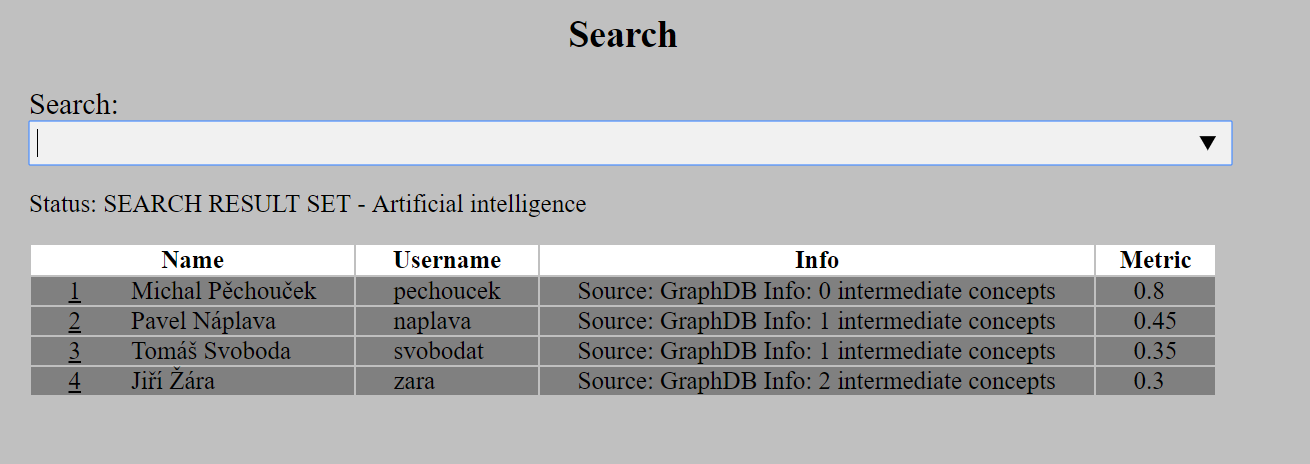
\includegraphics[width=\linewidth]{img/client.png}
	\caption{Snímek klientské části prototypu s načteným výsledkem hledání (zdroj autor)}
	\label{fig:client-screenshot}
\end{figure}

\section{Databáze}
% schema, zmínit mapování na doménový model [TODO možná: doménový model pro naší situaci, pro účely OOM]
Jak jsme zmínili výše, jako triplě-store databázi jsme zvolili GraphDB. V této sekci popíšeme ontologické schéma navržené pro naší databázi.\par
\subsection{Databázové schéma}
Již v kapitole č. \ref{chap:processing} jsme zmínili, že volbu ontologického schematu lze realizovat buď vlastní ontologií, existující ontologií, nebo kombinací obojího.\par
Podrobně naše řešení rozebereme v pozdějších sekcích této kapitoly. Zde však upozorníme na to, k čemu jsme konkrétně použili ontologie. V našem konkrétním řešení používáme ontologii v podstatě jako slovník, ve kterém jsou shromážděny koncepty provázané vazbami. V tomto slovníku poté vyhledáváme koncepty a hlavně jejich souvislosti.\par
Jak jsme již zmínili, tvorba slovníku nebo tezauru je typickým případem užití pro existující ontologii SKOS. Rozhodli jsme se, že pro náš prototyp použijeme tu.\par
Slovník bude obsahovat koncepty, zbývají nám tedy ostatní entity z našeho doménového modelu - znalost, osoba a pracoviště. Tyto budeme ukládat též do ontologií, jelikož toto datové úložiště již máme k dispozici a není třeba zvyšovat komplexnost systému další databází.\par
V příloze \ref{fig:ontology-scheme} je k vidění použité schéma, tzn. původní SKOS schéma (zdroj: \url{https://www.w3.org/2009/08/skos-reference/skos.rdf}) obohacené o další entity (osoba, pracoviště a znalost).
% Pro přehlednost není na obrázku kompletní SKOS schéma.
% [TODO (myslím, že to je pochopitelné a není třeba):Popis: schéma Odkaz na dokumentaci SKOS, krátce popsat entity a vazby]
\subsection{OOM}
Ontologicky-relační mapování probíhá z databáze na entity v balíčku \ctulst(none)!gdb_solution/model!, které jsou implementací rozhraní entit domény z balíčku \ctulst(none)!domain/model!. Tento programový vzor jsme zvolili, jelikož implementace SPI adaptérů se může v čase měnit. Model příslušného řešení tedy musí implementovat rozhraní modelu domény, nicméně může obsahovat další atributy, specifické pro konkrétní řešení. Na obrázku \ref{fig:concept} je celá situace schematicky zobrazena na entitě Koncept. Vidíme, že Koncept z databáze se se mapuje na třídu \ctulst(none)!ConceptGDB! z \ctulst(none)!gdb_solution/model! a s tou dále v \ctulst(none)!domain! pracujeme jako s implementací rozhraní \ctulst(none)!Concept!.
\begin{figure}[htbp!]
	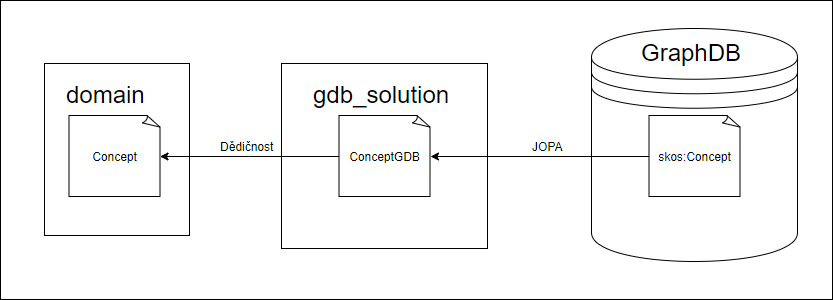
\includegraphics[width=\linewidth]{img/concept.png}
	\caption{Mapování objektů zobrazené schématicky, příklad na objektu Koncept (zdroj autor)}
	\label{fig:concept}
\end{figure}

% \subsubsection{Datový model - ontologie}
% konkrétní diagram tříd, možná schematicky udělat semantickou síť
% Zmínit, že řešení tohoto modulu se může různit, v další kapitole rozebereme naše konkrétní řešení, ale zde zmíníme datový model, ontologický, který použijeme, dá se říct něco o SKOS a alternativách
% Již konkrétní část řešení - konkrétní
% Datový model – návrh ontologie
% Ontologie
% Volba schema databáze
% - varianty SKOS apod. (Denis mi posílal prezentaci), např. http://xmlns.com/foaf/spec/
% - rozšířit SKOS o Person, Knowledge (možná bude potřeba)
% - protege

\section{Popis implementovaného řešení}
Výše jsme rozebrali části, ze kterých se navrhovaný systém skládá. V této sekci rozebereme, v jakých krocích vyhledávání lidí dle kompetencí probíhá a jednotlivé kroky popíšeme.\par
% Před tím než postup rozebereme, je důležité připomenout, že nejdůležitějším požadavek na navrhovaný systém byl požadavek na modularitu (\ref{furps}). Tento požadavek je zde z toho důvodu, že řešený problém je netriviální a je mnoho různých způsobů, jak jej řešit. V následující sekci představíme jedno z možných řešení, jedná se o variantu synchronního průběhu vyhledávání osob dle kompetencí (viz \ref{fig:sequence-synchronous}).\par
\subsection{Jednotlivé kroky vyhledávání}
\begin{enumerate}
    \item \textbf{Seznam konceptů} - klientská část vyšle požadavek na seznam konceptů, na které je možno se dále dotazovat
    \item \textbf{Příjem požadavku a odpověď} - \ctulst(none)!rest! modul požadavek přijme a předá jej \ctulst(none)!domain!, ta poté předá modulu \ctulst(none)!gdb_solution!, který vrací zpět skrz předchozí moduly seznam konceptů s názvem a identifikátorem
    \item \textbf{Vyhledání dle kompetence} - klientská část pošle identifikátor konceptu, pro který je třeba nalézt seznam kompetentních osob
    \item \textbf{Příjem požadavku} - \ctulst(none)!rest! modul požadavek přijme a předá jej \ctulst(none)!domain!, ta poté předá modulu \ctulst(none)!gdb_solution!
    \item \textbf{Zpracování požadavku} - hledaný koncept se využije jako parametr pro použitý databázový dotaz (vysvětleno níže), výsledek dotazu je ještě v komponentě \ctulst(none)!gdb_solution! dále zpracován (vysvětleno níže) a následně vrácen do \ctulst(none)!domain!
    \item \textbf{Návrat dat} - výsledek je vrácen jako seznam osob s vypočtenou sílou znalosti, příklad kompletního výsledku je možno vidět v příloze \ref{app:search-result}
\end{enumerate}

\subsection{SPARQL dotaz}
\subsubsection{Dotaz}
Součástí přílohy \ref{app:sparql-query} je použitý databázový dotaz v jazyce SPARQL. Nejpřímočařejší je popsat dotaz pomocí jeho výsledku. Dotaz vrací výčet konceptů ležících mezi vyhledávaným konceptem a danou osobou a váhu znalosti, kterou osoba k poslednímu z konceptů má. Jako hrana se v tomto průchodu používá relace \textit{semanticRelation}. Tato relace je součástí ontologie SKOS a je nejobecnější vazbou mezi dvěma koncepty, značí, že spolu dva koncepty významově souvisí.\par
Dotaz ve své podstatě prohledává po kružnicích okolí konceptu, ke kterému hledáme znalost, a vyhledává osoby, které se nachází maximálně čtyři \textit{semanticRelation} relace daleko od tohoto konceptu. Číslo čtyři v tomto nemá žádný význam, vzniklo empiricky, jelikož provázanost konceptů přes vazbu \textit{semanticRelation} je tak rozsáhlá, že u pěti již dotaz vrací příliš velký výsledek.
% [Argumentovat použití tohoto dotazu na místo hledán nejkratší cesty]
\subsubsection{Zpracování výsledku dotazu}
Výsledek dotazu je třeba uživateli interpretovat, dotaz vrací sílu znalosti k poslednímu konceptu, který leží mezi osobou a vyhledávaným konceptem, a výčet všech mezilehlých konceptů, neexistuje tedy jednotná metrika, dle které by bylo možné výsledek seřadit. Navíc ve výsledku dotazu se osoby opakují a ve finálním výsledku by se měla každá vyskytovat maximálně jednou.\par
\noindent Výslednou sílu znalosti $W$ jsme vypočítali následujícím vzorcem:
$$W=\frac{w}{n +1}$$
% $$I_K=\sum_{i=1}^{k}\sum_{j=1}^{q}r_i w$$
Kde $w$ je síla znalosti k poslednímu z konceptů a $n$ je počet mezilehlých konceptů.\par
% Vzniklý vzorec není pro naše zkoumání stěžejní, jelikož více než konkrétní výsledky chceme potvrdit, že naše řešení lze využít.\par
Výskyt duplicitních hodnot jsme vyřešili tak, že z celého výsledku bereme pro každou z osob vždy jen záznam s nejvyšším $W$.
% [možná diagram sekvencí - nemusí být]
\section{Rozšiřitelnost}
Z FURPS analýzy (\ref{furps}) vyplývá požadavek na modularitu systému, aby jednotlivé moduly (hlavně \ctulst(none)!gdb_solution!) byly jednoduše nahrazovány jinými implementacemi a podobně.\par
Pokud k takové změně dojde (konkrétně u SPI adaptéru), je třeba implementovat rozhraní potřebných SPI portů. Následně je třeba modifikovat konfiguraci v \ctulst(none)!application! a poskytnout Spring kontejneru příslušné nové implementace SPI adaptérů.
% - největší požadavek
% - ukázat, jak navázat, ukázky kódu
% Rozšiřitelnost projektu a modularita zvoleného řešení
% ukázat na příkladu, jak by šla aplikace rozšířit změnit, jak by se dalo na implementaci navázat
\section{Dokumentace projektu}
Dokumentace implementační části této práce vznikla na několika úrovních:
\begin{itemize}
    \item Javadoc - součástí odevzdaného programu
    \item Dokumentace návrhu a implementačních podrobností - kapitola č. \ref{chap:app-design} a č. \ref{chap:implementation} této práce
    \item Použité knihovny, technologie a nástroje jsou součástí přílohy \ref{app:technology-list}
    % [TODO: součástí příručka - možná]
\end{itemize}
% [TODO: dokumentace API]

\section{Shrnutí}
V této kapitole jsme rozebrali implementační podrobnosti námi realizovaného prototypu systému pro vyhledávání osob dle kompetencí na FEL ČVUT.\par
Prototyp jsme po částech popsali, představili jsme, jak je celý projekt strukturován a připojili jsme i popis technologií. V závěru této kapitoly jsme krok po kroku popsali použitý postup.

% inspirace: https://dspace.cvut.cz/bitstream/handle/10467/24264/F3-DP-2014-Jinoch-Vlastimil-prace.pdf?sequence=3&isAllowed=n

% TripleStore DB:
% https://www.ontotext.com/products/graphdb/editions/ - porovnání edic graphDB (včetně například podpory ellastic search)



%  jednotlivé technologie popsat a citovat, ukázky kódu (nenutit se do toho, je to místy dost strohé), popsat, co na vrstvách má správně probíhat! Technologie - výběr vhodného prostředí - na základě požadavků na program, program stack - frameworks...

    \chapter{Testování} \label{chap:testing}
V následující kapitole rozebereme testování.
% Klientská část slouží pouze pro demonstraci funkčnosti serverové, nejedná se o plnohodnotnou aplikaci, není třeba jí testovat.
Kapitola bude mít dvě části. V první z nich rozebereme obecně, jakým způsobem lze testovat hexagonální architekturu. V druhé části demonstrujeme některé z představených druhů testů na našem prototypu.
\section{Testování hexagonální architektury}
Alistar Cockburn, který hexagonální architekturu nejvíce prosadil, zmiňuje jako jeden z hlavních přínosů této architektury právě izolované testování. Primárně mluví o automatizovaném testování domény, odstíněném od ostatní infrastruktury (databáze, API jiných systémů) \cite{cockburn}. Doména obsahuje hlavní případy užití, je velmi výhodné je testovat izolovaně od všeho ostatního a hlavně automatizovaně.\par
\noindent Testování hexagonální architektury může probíhat na všech částech systému, nejen na doméně.
\paragraph{Rozdělení testování:}
\begin{itemize}
    \item Testování domény
    \item Testování SPI
    \item Testování API
\end{itemize}
\subsection{Testování domény}
Testy domény jsou architektonicky na stejné úrovni jako jsou API adaptéry, ve své podstatě se jedná o API adaptéry \cite{cockburn}. Tyto adaptéry volají implementaci API portů, které obsahují logiku, a tuto logiku testují. Logika (případy užití) je dále nabízena ostatním systémům, je tedy nutné jí otestovat.\par
V případě tohoto druhu testování je důležité doménu izolovat od ostatních vlivů, v podstatě se jedná o jednotkové testování. Ostatními vlivy jsou v tomto kontextu myšleny SPI adaptéry, které můžeme nahradit například mock objekty \cite{cockburn}. Jinými slovy můžeme SPI adaptéry, které slouží integraci s jinými systémy, nahradit dalšími adaptéry, které budou tuto integraci pouze předstírat a budou vracet námi definovaný správný výsledek.
\subsection{Testování SPI}
Poté co zajistíme doménu, je třeba zajistit, že SPI adaptéry budou poskytovat všechna data ve správné podobě (v podobě jako v mock objektech).\par
SPI adaptéry resp. moduly, které obsahují SPI adaptéry, mohou mít libovolnou vnitřní architekturu. Tuto architekturu je třeba testovat tak, jak je pro ní typické, a tak zajistit funkčnost SPI adaptérů.\par
Na klasické vrstevnaté architektuře (obdoba brownovy architektury \ref{tab:brown}) lze například provádět testování po jednotlivých vrstvách jako je tomu zvykem. Obvyklé je využití mock objektů, in-memory databází a obdobných technik.
\subsection{Testování API}
Posledním modulem, který zbývá jsou API adaptéry. Existují různé druhy těchto adaptérů, pro testování bereme v úvahu hlavně REST a GraphQL.\par
Tento druh testování se v případě malé aplikace může provést ručně. V komplikovanějších případech existují různé testovací knihovny a frameworky (například HttpClient - \url{http://hc.apache.org/httpcomponents-client-ga/index.html}). Tyto knihovny typicky volají API systému a kontrolují funkčnost, jako například návratové kódy.

\section{Testování implementované aplikace}
Prototyp aplikace, který jsme v rámci této práce vyvinuli se nejvíce opírá o modul \ctulst(none)!gdb_solution!, na ten je třeba se zaměřit při testování nejintenzivněji.\par
\noindent Oblasti naší aplikace k testování:
\begin{itemize}
    \item Persistentní vrstva modulu \ctulst(none)!gdb_solution!
    \item Logika modulu \ctulst(none)!gdb_solution!
    \item REST API
\end{itemize}
Samozřejmě je možné zapojit další druhy testů, vzhledem k rozsahu prototypu jsou však tyto tři úrovně dostačující.
% Hlavním důvodem, proč jsme další testy neimplementovali je fakt, že další integrace mezi moduly jsou bez jakékoliv složitější logiky vhodné k testování.
\section{Průběh testu}
Testy jsou v naší aplikaci vždy rozděleny na tři části:
\begin{itemize}
    \item \textit{arrange} - příprava akce (inicializace instancí, jiné integrační akce a podobně)
    \item \textit{act} - testovaná akce
    \item \textit{assert} - ověření výsledku
\end{itemize}
\subsection{Testování persistentní vrstvy}
Integrační testy persistentní vrstvy jsou v kontextu naší práce klíčové. Hlavně proto, že nepoužíváme jiné datové úložiště než graphDB. Navíc hlavní dotaz pro vyhledávání osob dle znalosti probíhá pomocí SPARQL na této úrovni.\par
Při testování integrace se používá testovací repozitář GraphDB. Hlavním důvodem je, že integrační testy musí mít izolované prostředí, nezávislé na ostatních (produkčních a podobně).
\subsubsection{Pokrytí testy}
Jelikož je modul \ctulst(none)!gdb_solution/dao! naprogramován genericky, je poměrně přímočaré otestovat společné metody dao objektů (CRUD). Individuálně se testují jen specifické funkce jednotlivých dao objektů, v našem případě jen \ctulst(none)!PersonDao!.
\subsubsection{Příklad integračního testu s popisem}
Níže je k vidění příklad integračního testu, který testuje metodu \ctulst(none)!findAll!. Test probíhá nad entitou \ctulst(none)!PersonGDB!, nicméně se jedná o generickou metodu, testujeme tedy i ostatní entity. V části \textit{arrange} připravujeme prostředí, tedy vytváříme tři instance entity osoba a zapisujeme je do testovacího repozitáře graphDB. V části \textit{act} čteme všechny záznamy osob z repozitáře graphDB. V části \textit{assert} kontrolujeme obsah výsledku s obsahem původního seznamu, používáme k tomu funkce \ctulst(none)!assertEquals! a \ctulst(none)!assertTrue! z knihovny JUnit 4 (\url{https://junit.org/junit4/}). 
\begin{lstlisting}[language=JAVA, caption= Příklad integračního testu, captionpos=b]
    @Test
    public void findAllReturnsAllExistingInstances() {
        //arrange
        final List<PersonGDB> persons = new ArrayList<>();
        persons.add(new PersonGDB("Dominik", "Kouda", "koudadom"));
        persons.add(new PersonGDB("Dominik2", "Kouda1", "koudadom1"));
        persons.add(new PersonGDB("Dominik1", "Kouda2", "koudadom2"));
        //act
        personDao.persist(persons);
        final List<PersonGDB> result = personDao.findAll();
        //assert
        assertEquals(persons.size(), result.size());
        boolean found = false;
        for (PersonGDB person : persons) {
            for (PersonGDB person2 : result) {
                if (person.equals(person2)) {
                    found = true;
                    break;
                }
            }
            assertTrue(found);
        }
    }
\end{lstlisting}
% [TODO: možná doplnit test metody getPeopleByKnowledge]
\subsection{Testování logiky}
Logikou je v modulu \ctulst(none)!gdb_solution! myšlena hlavně třída \ctulst(none)!KnowledgeDTOList!. Tato třída reprezentuje množinu znalostí. Množina má navíc tu vlastnost, že v případě vložení duplicitního záznamu, zůstane v množině vždy prvek s větší sílou znalosti. Tato třída se využívá při vyhledávání osob dle znalosti ke kompletaci výsledku SPARQL dotazu.\par
V testu níže lze vidět obdobný postup jako tomu bylo výše. V tomto konkrétním příkladu kontrolujeme, že při přidání jedné osoby vícekrát se aktualizuje její síla znalosti, byla-li přidávána vyšší.
\begin{lstlisting}[language=JAVA, caption= Jednotkový test aplikační logiky modulu gdb\_solution, captionpos=b]
    @Test
    public void addsOnlyHighest() {
        //arrange
        KnowledgeDTOList list = new KnowledgeDTOList();
        PersonGDB p1 = new PersonGDB("Dominik", "Kouda", "koudadom");
        PersonGDB p2 = new PersonGDB("Dominik2", "Kouda1", "koudadom1");
        PersonGDB p3 = new PersonGDB("Dominik1", "Kouda2", "koudadom2");
        //act
        list.add(new KnowledgeDTO(p1, 0.5, new HashSet<>()));
        list.add(new KnowledgeDTO(p2, 0.5, new HashSet<>()));
        list.add(new KnowledgeDTO(p3, 0.6, new HashSet<>()));
        list.add(new KnowledgeDTO(p1, 0.7, new HashSet<>()));
        //assert
        assertEquals(3, list.size());
        boolean success = false;
        for(KnowledgeDTO dto: list.getKnowledgeDTOs()){
            if(dto.getOwner().equals(p1) && 
                    dto.getWeightOfKnowledge() == 0.7){
                success = true;
            }
        }
        assertTrue(success);
    }
}
\end{lstlisting}
Tímto druhem testů je otestována správná funkce této třídy. Konkrétně je to kontrola duplicit v množině a maximalizace síly znalosti každé osoby v množině, při postupném přidávání.
\subsection{Testování REST API}
API má dva základní případy použití - vrácení seznamu všech konceptů a vyhledání osob dle zvoleného konceptu. Vzhledem k tomu, že tato část aplikace není příliš složitá, rozhodli jsme se pro ruční otestování.\par
\subsubsection{Scénáře}
\begin{table}[h!]
\begin{ctucolortab}
% \begin{tabular}{|l|l|m{3cm}|l|m{2,75cm}|}
\begin{tabularx}{0.95\linewidth}{X|X|X}
\bfseries Testovaný případ  & \bfseries Očekávaný výsledek & \bfseries Výsledek testu\\\hline 
    % \hline
    %  & Forma dat & Dostupnost dat & Aktualizováno & Správce \\ \hline
    Dotaz na všechny koncepty & Seznam všech konceptů ve formátu JSON & OK \\\hline
    Vyhledání dle konceptu (existujícího) & Seznam osob ve formátu JSON & OK \\\hline
    Vyhledání dle konceptu (neexistujícího) & Status 404 & Nalezena chyba \\
\end{tabularx}
\end{ctucolortab}
	\caption{Tabulka testovacích případů pro REST API}
	\label{tab:rest-testing}
\end{table}
Testování proběhlo bez větších problémů, byla nalezena chyba při dotazu na neexistující koncept. Chyba byla opravena.
\section{Shrnutí}
V této kapitole jsme shrnuli testování naší aplikace. V úvodu jsme popsali výhody testování hexagonální architektury a používané principy. V druhé části kapitoly jsme popsali testování serverové části našeho prototypu. Vzhledem k rozsahu prototypu jsme nepoužili všechny druhy testů, které je možné pro hexagonální architekturu implementovat.\par
Implementace testů proběhla bez problémů, nalezené chyby jsme opravili. Ruční testování proběhlo též bez komplikací, nalezené chyby jsme opravili.





% \subsection{Další výhody testování}
% Může být například testovací profil jen pro účely UI testování, který nezdržuje žádná databáze apod. zkrátka \cite{cockburn}

% \begin{itemize}
%     \item SPI - infrastrukturu lze nahradit různými způsoby - dummy, mock (viz fowler), jiný zdroj (jiný typ databáze...), skutečná databáze s testovacími daty
%     \item API - Lze nahradit testovací frameworkem (testování domény, je v podstatě na stejné úrovni jako je samotné API, je v podstatě API adaptérem)
% \end{itemize}





% Jak jsme již napsali v předchozí kapitole \ref{chap:implementation}: Účelem implementační části této práce je dokázat, že navržené řešení je možno použít a že skutečně může po dalších rozšířeních fungovat v praxi. K testování toho není mnoho, proto jsme zvolili pouze testovací úrovně, které dle nás mají pro náš rozsah smysl.\par
% Důležité je zmínit, že zvolená hexagonální architektura patří mezi nejlépe testovatelné, obzvlášť díky své modularitě a zapouzdření.
% % testování hexagonální architektury teoreticky (jeden zdroj tam byl)




    \chapter{Budoucí práce} \label{future}
\section{Neprobraná témata}
Během práce jsme narazili na několik témat, které jsme z rozsahu této práce vyloučili. Není však pravda, že tato témata nemají potenciál, proto je zmiňujeme zde.\par
\subsection{Osobnost a dovednosti}
V sekci zabývající se reprezentací dat (kapitola č. \ref{chap:data_representation}), jsme se rozhodli zanedbat část z vlivů na kompetence osoby - osobnost (povaha, motivy). Toto téma je velmi komplexní z hlediska reprezentace těchto dat i z hlediska potenciálních datových zdrojů - vlastní popis sama sebe, reference zaměstnavatele a jiné.\par
Ve stejné sekci jsme vyloučili dovednosti, v této práci jsme je v podstatě sloučili se znalostmi. Znalosti však nejsou totéž co dovednosti. Společně se zkušenostmi by dovednosti měli být dalším důležitým okruhem, který staví na znalostech a popisuje, jak je osoba umí využívat.
\subsection{Vlastní datový zdroj}
V sekci týkající se datových zdrojů (kapitola č. \ref{chap:data-sources-analysis}) jsme rozebrali primárně zdroje, které již existují. Je možné vytvořit vlastní zdroj - např. na základě vstupů od osob (formulář pro tvorbu profilu v databázi kompetencí). Případně je možné vlastní zdroj vytvořit z existujících - anotace existujících dat a podobně.
\subsection{Nestrukturovaná data}
V sekci zpracování dat (kapitola č. \ref{chap:processing}), konkrétně jejich transformace do požadovaných formátů, jsme se zaměřili pouze na serializovaná/strukturovaná data. Data však nejsou vždy k dispozici v takto strojově dobře čitelném formátu. Často jsou nestrukturovaná a nevhodná pro strojové zpracování např. prostý text. Zde se jedná o problematiku sémantické anotace dat, zpracování přirozeného jazyka a podobně.
Jedná se např. o zdroje jako jsou životopisy nebo osobní stránky.
\subsection{Transformace dat}
V rámci návrhu systému v kapitole č. \ref{chap:app-design} jsme pro komplexnost nerozebrali část transformace dat z existujících zdrojů do zvolené reprezentace (nebylo to součástí zadání této práce). Pokud má systém fungovat v praxi, je třeba data vhodným způsobem získávat a transformovat. Toto souvisí s bodem výše, data mohou být buď strukturovaná, nebo bude třeba je vhodným způsobem strukturovat.

\section{Navazující práce}
V rámci této práce jsme potvrdili, že námi zvolený způsob lze po dalších rozšířeních aplikovat v praxi. V této sekci shrneme, v jakých oblastech lze řešení dále posouvat.
\section{Výkon}
Triple-store databázi jsme použili pro uložení veškerých dat - osoby, pracoviště i znalosti. Do budoucna bude lepší ukládat v ní jen znalostní bázi. Osoby, pracoviště a další potřebná data je lepší strukturovat v jiném úložišti.\par
% V rámci našeho řešení jsme nekladli důraz na implementační detaily, jelikož se jedná více o prototyp, který prokazuje funkčnost. Při vyhledávání bude lepší používat parametry jako je offset a limit, pro efektivnější práci s koncepty.
\section{Zvolený potup}
Námi zvolený postup popsaný v kapitole č. \ref{chap:implementation} má jisté nedostatky. Zároveň je také důležité vyzkoušet jiná možná řešení, abychom mohli rozhodnout, které je nejefektivnější.\par
\paragraph{Další oblasti pro rozvoj:}
\begin{itemize}
    \item Fulltext - v GraphDB nebo v jiné databázi; Elastic search - \url{https://www.elastic.co/}
    \item Jiné způsoby agregace dat pro získání výsledných metrik (síla znalosti apod.)
    \item Zapojení dalších druhů databází (např. dokumentové, relační)
    \item Zapojení vyvozování (angl. reasoning) pro validaci konzistence dat a získávání dalších dat v triple-store databázi
\end{itemize}


% - Bez ohledu na řešení BP by bylo dobré zamyslet se nad využitím http://graphdb.ontotext.com/documentation/standard/plug-ins.html - fulltext, mongo, semantic search
% - pomocí OWL mohu data více popisovat - jejich omezení, závislosti apod.
% NÁPADY:
% - Vyhledávat klíčová slova pomocí ELASTIC SEARCH, ty až poté propojovat s koncepty v OntoDB
% -----> UC: 
%           1. Uživatel zadá klíčové slovo
%           2. Systém klíčové slovo vyhledá mezi dostupnými daty (např. v ES datasource) a zjistí k čemu se dané slovo váže (buď to bude v ellastic search přímo takto uloženo, nebo využije některou z externích služeb, než nenalezne slovo, které se váže k zadanému a zároveň pro něj existje koncept v ontoDB)
%           3. Systém vrátí seznam relevantních lidí (dle toho, co našel v ES (třeba jen autorství), nebo toho, co je v ontoDB u konceptu jako vlastník) nějak seřazeno dle váhy záznamu, ve kterém jsme info našli
% - DB dokumentů s klíčovými slovy, zkusit využít SKOS opravdu jen jako slovník, v kterém to vyhledám a pak klíčová slova naleznu někde v mongu v těch dokumentech (např. v těch vědeckých pracích)
% HINTY:
% - skos:Concept is an instance of owl:Class

% BP:
% Myslím, že vyhledávání budu realizovat nějak takhle:

% 1. Uživatel záda klíčová slova (jednoduchý string, případně sousloví oddělené mezerou, reprezentující jeden koncept, např. Umělá inteligence)
%  - toto se dá diskretizovat pomocí našeptávače na straně klienta - (to udělám asi nejdříve, poté se budu zabývat spojitým protorem slov)
% 2. Dle zadaného vyhledám koncept (GRAPHDB má něco pro fulltext search/semantic search, zkusím to)
% 3. Naleznu objekty knowledge v okolí konceptu a dle vzdálenosti a typu vazeb a atributu weight jim přidělím nějakou relevanci (double <0,1>)

% 4. Dle této relevance potom seradim osoby vážící se k objektům knowledge  a jejich seřazený seznam vrátím.

% Udělat si vlastní slovník SKOS - jednodušší
% Postup s DB: (viz papír)
% nejdříve se zeptat relační DB, na přímé vazby mezi hledaným konceptem a lidmi

% 	1. Vyselectovat si podgraf - od osob k hledanému konceptu
% 	2. Vyhledat cesty k hledanému konceptu, vypočítat váhu (zapojit veličinu - délku cesty, váhu znalosti, případně typy vazeb na cestě (defaultně vzít skos:semanticRelation))

% alternativa:
% 	1. Vyselectovat si podgraf okolo hledaného konceptu, třeba 1-5 poloměr
% 	2. Vyhledat blízké objekty knowledge, vypočítat váhu

% V obou případech si ukládat koncepty a lidi do relační DB, prohledávání grafu realizovat mimo DB - vyexportovat si data



 




    % \afterpage{\blankpage}
	\chapter{Závěr}
Tato práce měla tři základní cíle. Prvním cílem bylo \textit{zanalyzovat problematiku vyhledávání osob a pracovišť dle kompetencí}. Tento cíl jsme splnili v první části, kdy jsme celý problém rozdělili na dílčí úkoly, a ty jsme postupně rozebrali. Začali jsme konceptuálním modelem celého problému, ze kterého jsme byli schopni lépe pochopit problematiku. Dále jsme zanalyzovali možnosti reprezentace kompetencí resp. znalostí, postupovali jsme od těch jednodušších (sémantické sítě) k těm složitějším (deskripční logika). V této části jsme jako nejvhodnější reprezentaci pro náš případ zvolili ontologie.  Hlavně proto, že jako jediný formální jazyk pro reprezentaci znalostí mají praktickou podporu technologií jako jsou RDF, OWL a SKOS. \par
Dále jsme zanalyzovali možné datové zdroje, zejména zdroje znalostí osob a znalostní báze. V této části jsme zjistili, že znalosti osob lze v akademickém prostředí nejlépe získat prostřednictvím vědeckých publikací a jiných výstupů vědecké činnosti. V komerčním prostředí se pro naše účely mohou vyskytovat znalostní systémy. Nejrozsáhlejší zdroje znalostní báze jsou na globální úrovni DBpedia a WordNet. Zjistili jsme také, že zdroje strukturovaných dat jsou často velmi omezené a že práce s nestrukturovanými daty jako je prostý text vyžaduje další zpracování (sémantická anotace a podobně).\par
Nakonec jsme se zabývali zpracováním dat. Rozebrali jsme jejich transformaci do ontologií pomocí nástrojů jako je OntoRefine. Následně jsme rozebrali jazyk SPARQL, který je klíčový v oblasti práce s ontologickými daty (RDF triply) a umožňuje provádět CRUD operace. V závěru této sekce jsme ještě zmínili obecný způsob získání síly znalosti, která je klíčovou metrikou při porovnávání znalostí více osob.
\par
Druhý cíl \textit{navrhnout systém pro vyhledávání osob a pracovišť dle kompetencí a provést rešerši dostupných dat} jsme naplnili ve druhé části práce. Nejdříve jsme rozebrali datové zdroje dostupné na FEL ČVUT. Klíčové jsou v tomto ohledu systémy Usermap a V3S. Systém Usermap může díky svému API sloužit jako zdroj osob a pracovišť. Systém V3S obsahuje rozsáhlou databázi vědecké činnosti na ČVUT. Dalším zjištěním v této části práce bylo, že na ČVUT neexistuje žádné jednotné rozhraní pro získávání nevědeckých dat o zaměstnancích - životopisy, osobní stránky a podobně.\par
Na analýzu datových zdrojů jsme navázali návrhem systému pro vyhledávání dle kompetencí. Systém jsme rozebrali počínaje požadavky, hlavním z nich je funkční požadavek na samotné vyhledávání, další důležitý je implementační požadavek na modularitu celého systému. Důraz na modularitu klademe, protože vyhledávání dle kompetencí je komplikovaný problém a není zjevné, kolik možných řešení existuje a jak je lze kombinovat.\par
Dále jsme postupovali přes případy užití a wireframy k výběru architektury. Požadavek na modularitu systému byl hlavním důvodem, proč jsme se odklonili od klasické vrstevnaté architektury. Nejdříve jsme rozebrali cibulovou architekturu, která je vzhledem ke svému nízkému provázání (angl. decoupling) vhodným kandidátem pro systémy jako je ten náš. Nakonec jsme zvolili variantu této architektury, totiž architekturu hexagonální. Tato architektura navíc ještě definuje způsob komunikace pomocí portů a adaptérů, což se v našem případě hodí. Hexagonální architekturu jsme tedy zevrubně představili a následně jí aplikovali na náš případ.\par
V poslední části práce jsme rozebrali prototyp navržené aplikace, který jsme implementovali. Prototyp má dvě části, server a klient. Demonstrovali jsme na něm funkčnost navržené aplikace. Jako technologii pro serverovou část jsme zvolili programovací jazyk JAVA, který vyhovuje technologickému prostředí ČVUT FEL. Pro ukládání dat pomocí ontologií jsme využili existující \textit{triple-store} GraphDB, jako schéma jsme použili ontologii SKOS rozšířenou o několik našich entit. Nakonec jsme v poslední kapitole rozebrali testování hexagonální architektury, nejdříve obecně a následně jsme některé z technik demonstrovali na našem prototypu.\par
Splnili jsme všechny stanovené cíle. Rozebrali jsme zevrubně celý problém vyhledávání dle kompetencí, navrhli systém, který tuto problematiku řeší a implementovali a otestovali prototyp pro FEL ČVUT. Nakonec jsme v kapitole budoucí práce shrnuli, jak na tuto práci navázat. Největší otázkou pro budoucí práce zůstává transformace existujících dat do zvolených struktur, do RDF triplů, a jejich následné začlenění do systému.






% Tato práce měla tři základní cíle. Prvním cílem bylo \textit{zanalyzovat problematiku vyhledávání osob a pracovišť dle kompetencí}. Tento cíl jsme splnili v první části této práce, kdy jsme celý problém rozdělili na dílčí úkoly a ty jsme postupně zanalyzovali. Klíčovou byla v této části volba reprezentace kompetencí resp. znalostí. Rozhodli jsme se je reprezentovat pomocí ontologického formálního jazyka. Při řešení dalších dílčích úkolů v první části jsme provedli rozbor každého problému a rešerši existujících technologií.\par
% Druhý cíl \textit{navrhnout systém pro vyhledávání osob a pracovišť dle kompetencí a provést rešerši dostupných dat} jsme naplnili v druhé části práce, konkrétně potom v kapitolách \ref{chap:data-sources-analysis} a \ref{chap:app-design}. V těchto kapitolách jsme zevrubně popsali potenciální datové zdroje a popsali jsme návrh systému.\par
% Implementovaný prototyp je přiložen k této práci na CD nosiči (příloha \ref{app:cd-content}). Dokumentace a popis prototypu jsou obsaženy v kapitolách \ref{chap:implementation} a \ref{chap:testing}. Tyto výstupy náleží k poslednímu cíli této práce - \textit{implementovat prototyp systému pro vyhledávání osob a pracovišť dle kompetencí pro FEL ČVUT}.\par
% Způsob jakým na tuto práci navázat a rozvinout její výstupy (implementační i teoretické) jsme shrnuli v kapitole č. \ref{future}.

% [Propojit to nějak s pokyny k vypracování]


% Cílem naší práce bylo vyřešit problematiku vyhledávání osob a pracovišť dle kompetencí na FEL ČVUT.\par
% Celou problematiku jsme v první části práce rozebrali v jednotlivých dílčích krocích. Klíčovou byla v této části volba reprezentace kompetencí resp. znalostí. Rozhodli jsme se je reprezentovat pomocí ontologického formálního jazyka. Při řešení dalších dílčích úkolů v první části jsme provedli rozbor každého problému a rešerši existujících technologií.\par
% Na první část jsme navázali v druhé polovině práce. Zde jsme již přistoupili ke konkrétnímu návrhu systému pro řešení celé agendy. Navrhli jsme obecnou architekturu systému pro vyhledávání osob dle kompetencí. Dále jsme popsali implementační část této práce, jejíž cílem bylo demonstrovat, že návrh je možné implementovat a skutečně funguje. Implementovaný systém pro vyhledávání kompetencí na FEL ČVUT je důkazem funkčnosti a po dalších rozšířeních může sloužit účelu, ke kterému byl navržen.\par
% Způsob jakým na tuto práci navázat a rozvinout její výstupy (implementační i teoretické) jsme shrnuli v příloze \ref{future}.
	
	\bibliographystyle{acm}
	\bibliography{ctubib}
	
	
	
\nomenclature{FEL ČVUT}{Fakulta elektrotechnická Českého vysokého učení technického v Praze}
\nomenclature{FIT ČVUT}{Fakulta informačních technologií Českého vysokého učení technického v Praze}
\nomenclature{FOL}{Logika prvního řádu (angl. First order logic)}
\nomenclature{CRUD}{Operace vytvoření, čtení, změna a vymazaní (angl. create, read, update a delete)}
\nomenclature{SKOS}{Systém pro organizaci znalostí (angl. Simple Knowledge Organization System)}
\nomenclature{OWL}{Webový ontologický jazyk (angl. Web Ontology Language)}
\nomenclature{SPARQL}{Protokol a RDF dotazovací jazyk (angl. Protocol and RDF Query Language)}
\nomenclature{RDF}{Framework pro popis zdrojů (angl. Resource Description Framework)}
\nomenclature{XML}{Rozšiřitelný značkovací jazyk (angl. Extensible Markup Language)}
\nomenclature{UFO}{Unifikovaná základní ontologie (angl. Unified Foundational Ontology)}
\nomenclature{URI}{Uniformní identifikátor zdroje (angl. Uniform Resource Identifier)}
\nomenclature{JSON-LD}{Javascriptová objektová notace pro propojená data (angl. JavaScript Object Notation for Linked Data)}
\nomenclature{UML}{Unifikovaný modelovací jazyk (angl. Unified Modelling Language)}
\nomenclature{API}{Rozhraní pro programování aplikací (angl. Application Programming Interface), v našem kontextu spíše webová služba nebo rozhraní pro poskytování dat}
\nomenclature{SPI}{Rozhraní poskytovatele služby (angl. Service Provider Interface)}
\nomenclature{HTTP}{Hypertext Transfer Protokol}
\nomenclature{REST}{Representational State Transfer (bez překladu)}
\nomenclature{GDPR}{Obecné nařízení o ochraně osobních údajů (angl. General Data Protection Regulation)}
\nomenclature{URL}{Jednotná adresa zdroje (angl. Uniform Resource Locator)}
\nomenclature{IdM}{Správa identit (angl. Identity Management)}
\nomenclature{HTML}{Hypertextový značkovací jazyk (angl. Hypertext Markup Language)}
\nomenclature{CSS}{Kaskádové styly (angl. Cascading Style Sheets)}
\nomenclature{ORM}{Objektově-relační mapování (angl. Object-relational mapping)}
\nomenclature{OOM}{Ontologicko-relační mapování (angl. Object-ontological mapping)}

\printnomenclature

	
	
% 	\printglossary[type=\acronymtype]
	
	
\appendix
\chapter{Konceptuální datový model}
\begin{figure}[htbp!]
	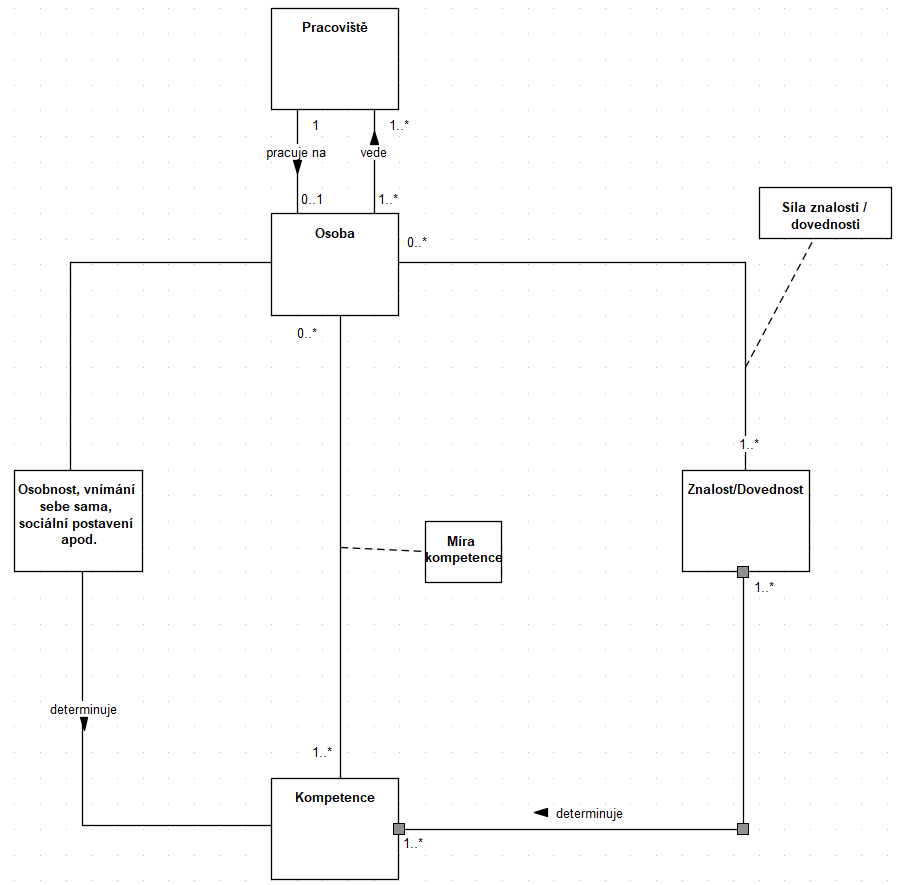
\includegraphics[width=\linewidth]{img/data_diagram.png}
	\caption{Diagram konceptuálního modelu (zdroj autor)}
	\label{fig:conceptual_appendix}
\end{figure}

% \chapter{Příklad ontologie}
% \begin{sidewaysfigure}[htbp!]
% 	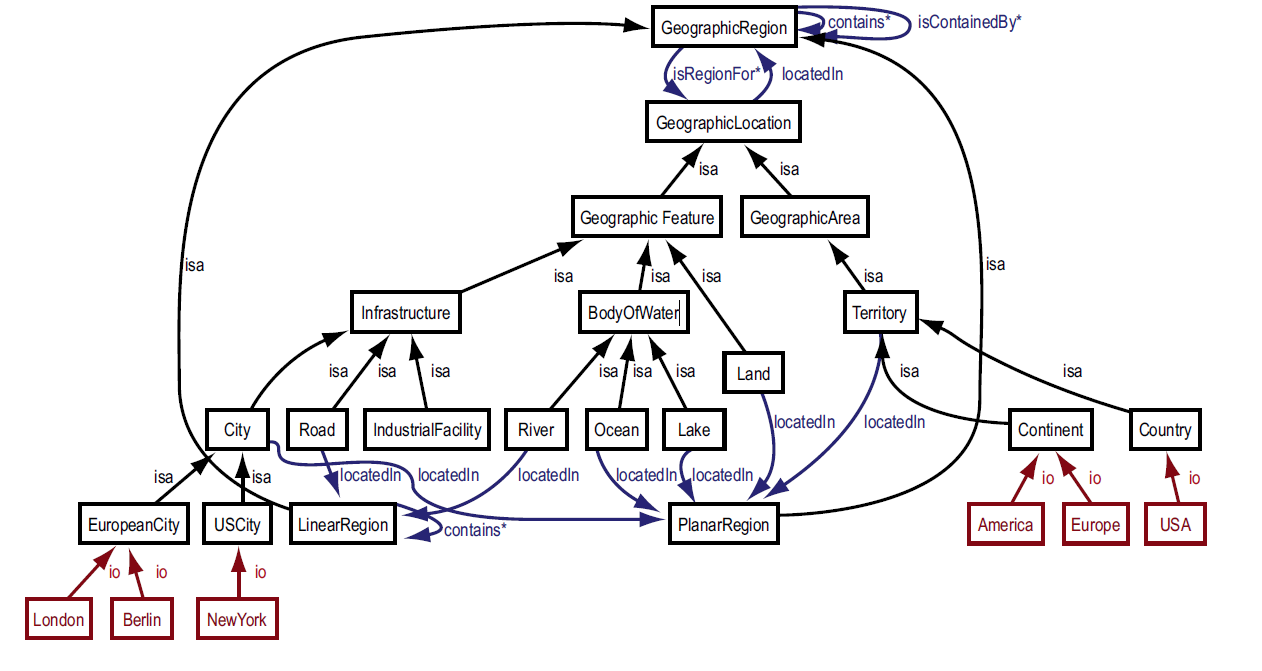
\includegraphics[width=0.75\linewidth]{img/ontology.png}
% 	\caption{Příklad geografické ontologie (zdroj \cite{Stephan2007})}
% 	\label{fig:ontology_example}
% \end{sidewaysfigure}

\chapter{SKOS vizualizace}
\begin{sidewaysfigure}[htbp!]
	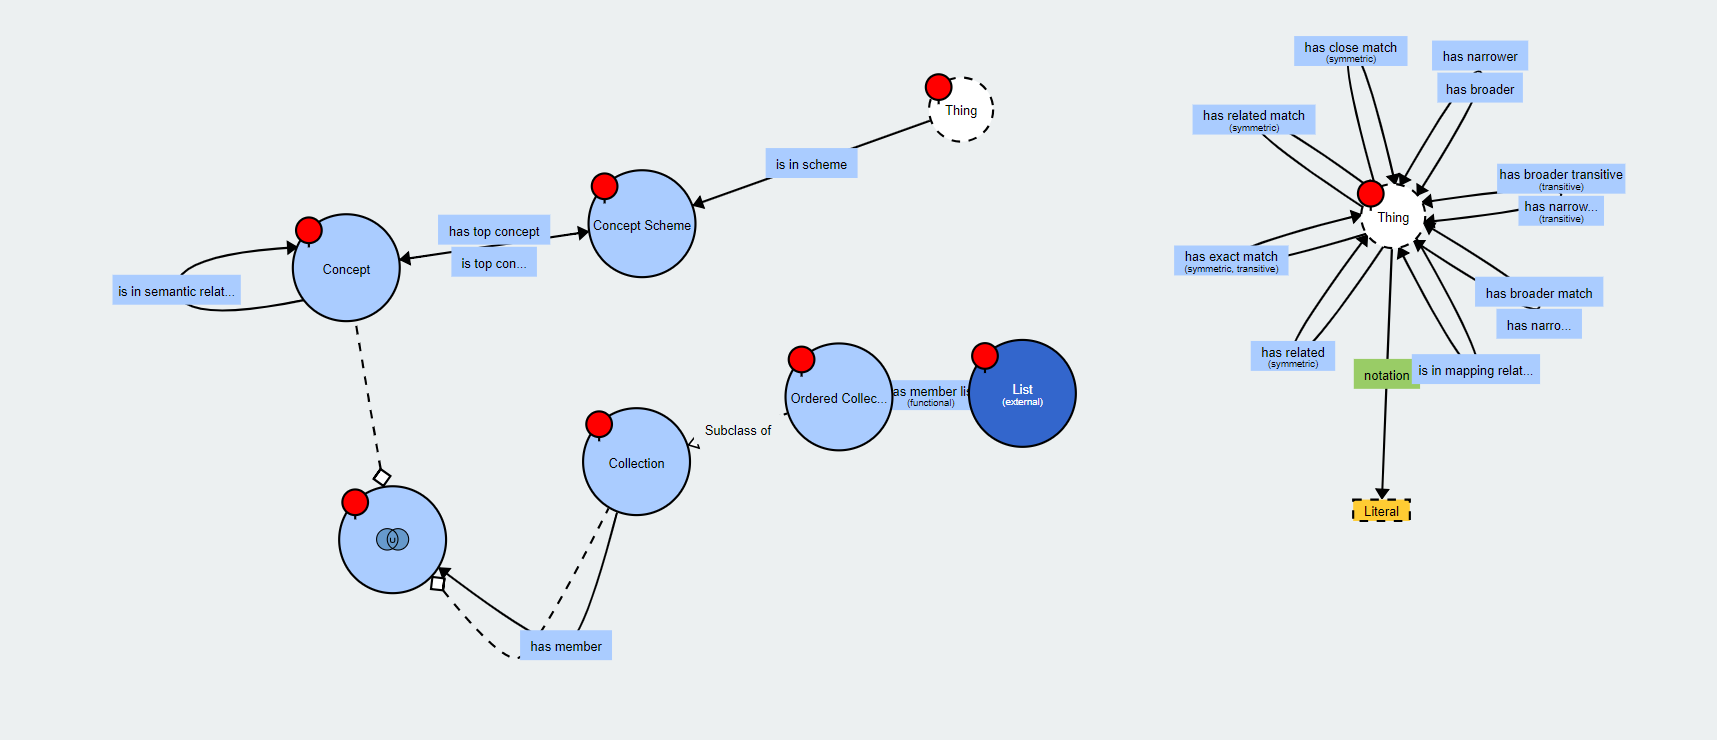
\includegraphics[width=0.9\linewidth]{img/SKOS-ontology.png}
	\caption{Ontologie SKOS (zdroj: \url{https://www.w3.org/2009/08/skos-reference/skos.rdf} použitý nástroj: \url{http://www.visualdataweb.de/webvow})}
	\label{fig:SKOS-ontology}
\end{sidewaysfigure}

\chapter{Diagram komponent}
\begin{sidewaysfigure}[htbp!]
	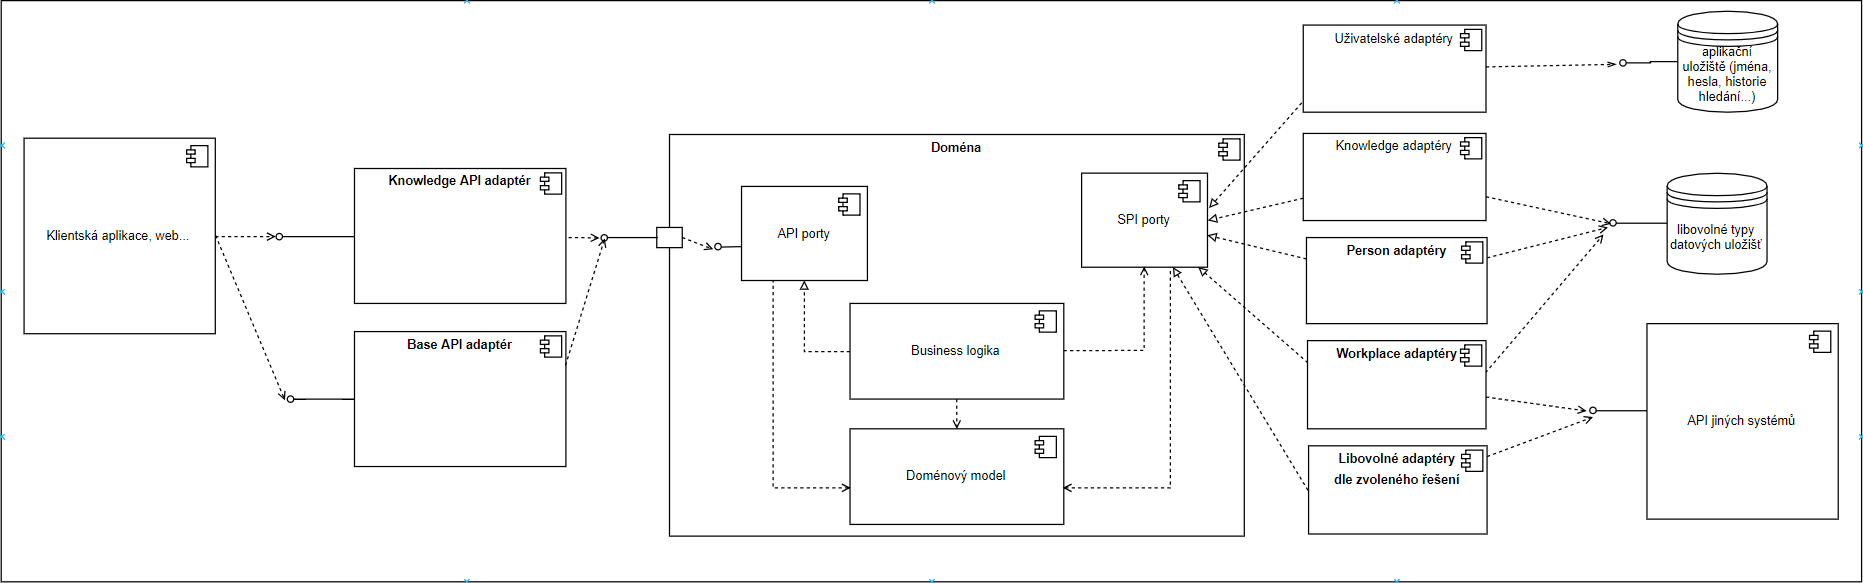
\includegraphics[width=\linewidth]{img/component.png}
	\caption{Diagram komponent (zdroj autor)}
	\label{fig:component-model}
\end{sidewaysfigure}

\chapter{Sekvenční diagram}  \label{appendix:sequence}
\begin{sidewaysfigure}[htbp!]
	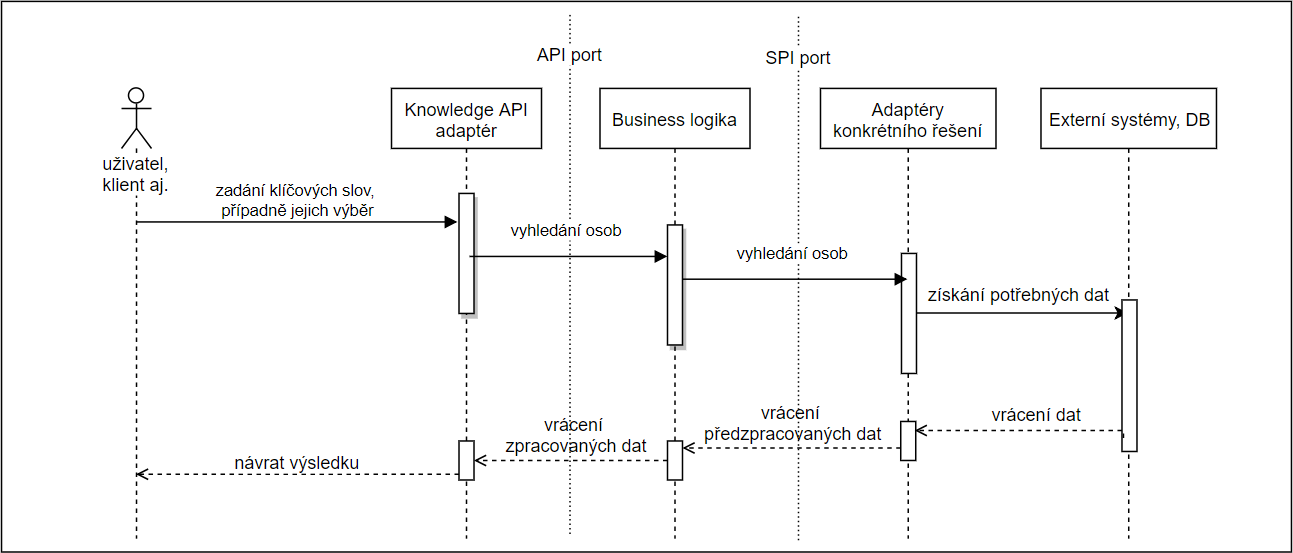
\includegraphics[width=\linewidth]{img/sequence-synchronous.png}
	\caption{Synchronní verze sekvenčního diagramu (zdroj autor)}
	\label{fig:sequence-synchronous}
\end{sidewaysfigure}

\begin{sidewaysfigure}[htbp!]
	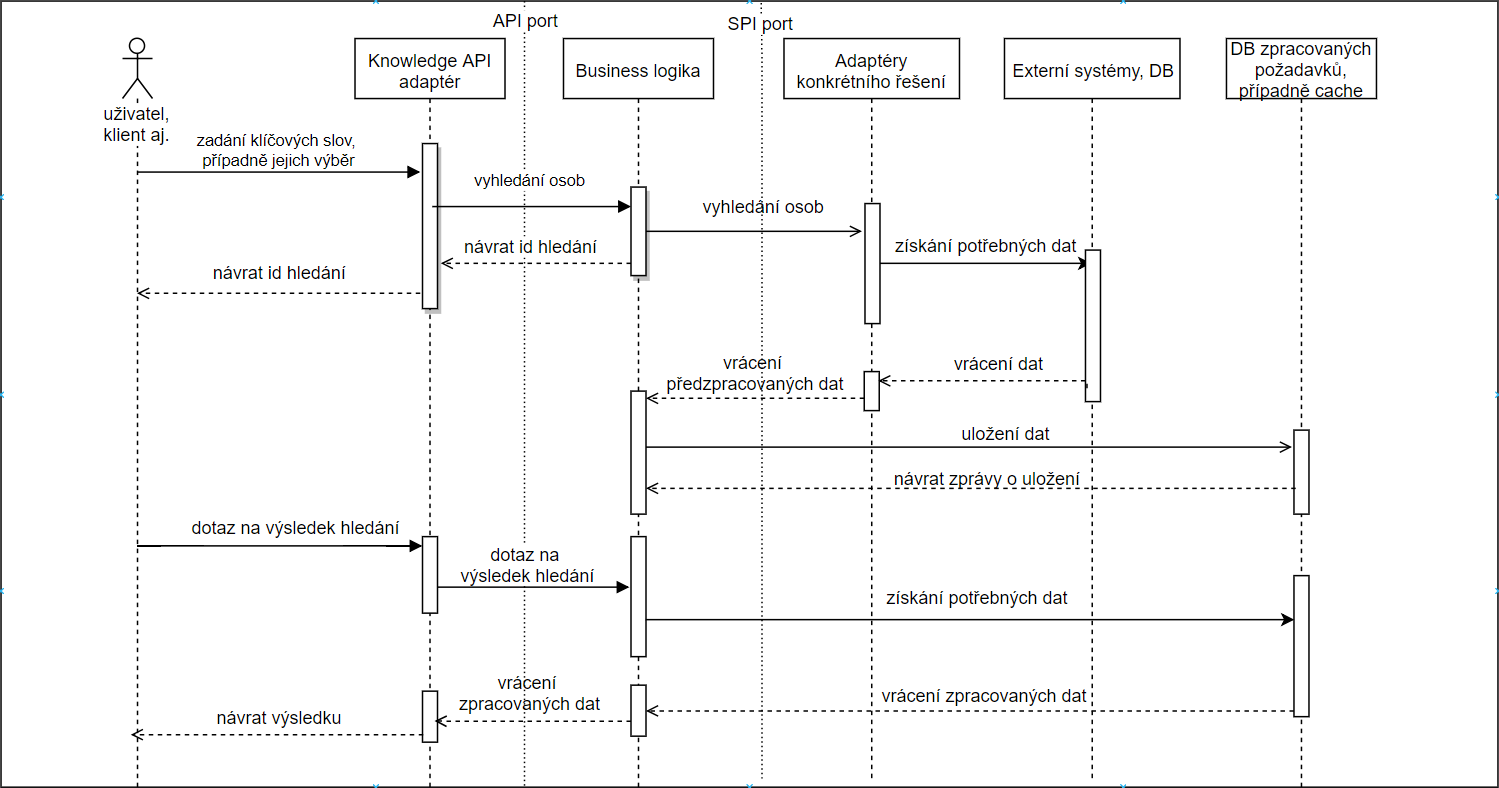
\includegraphics[width=\linewidth]{img/sequence-asynchronous.png}
	\caption{Asynchronní verze sekvenčního diagramu (zdroj autor)}
	\label{fig:sequence-asynchronous}
\end{sidewaysfigure}

\chapter{Doménový model}
\begin{figure}[htbp!]
	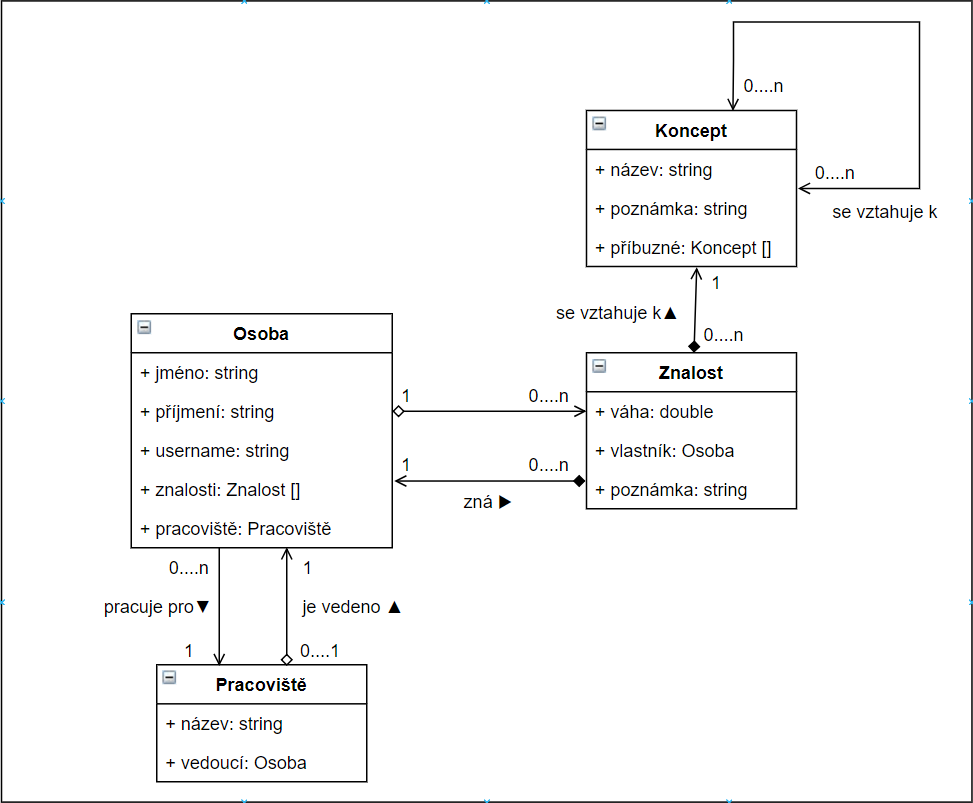
\includegraphics[width=\linewidth]{img/domain.png}
	\caption{Doménový model (zdroj autor)}
	\label{fig:domain-model}
\end{figure}

\chapter{Diagram komponent pro naše řešení FEL ČVUT}
\begin{sidewaysfigure}[htbp!]
	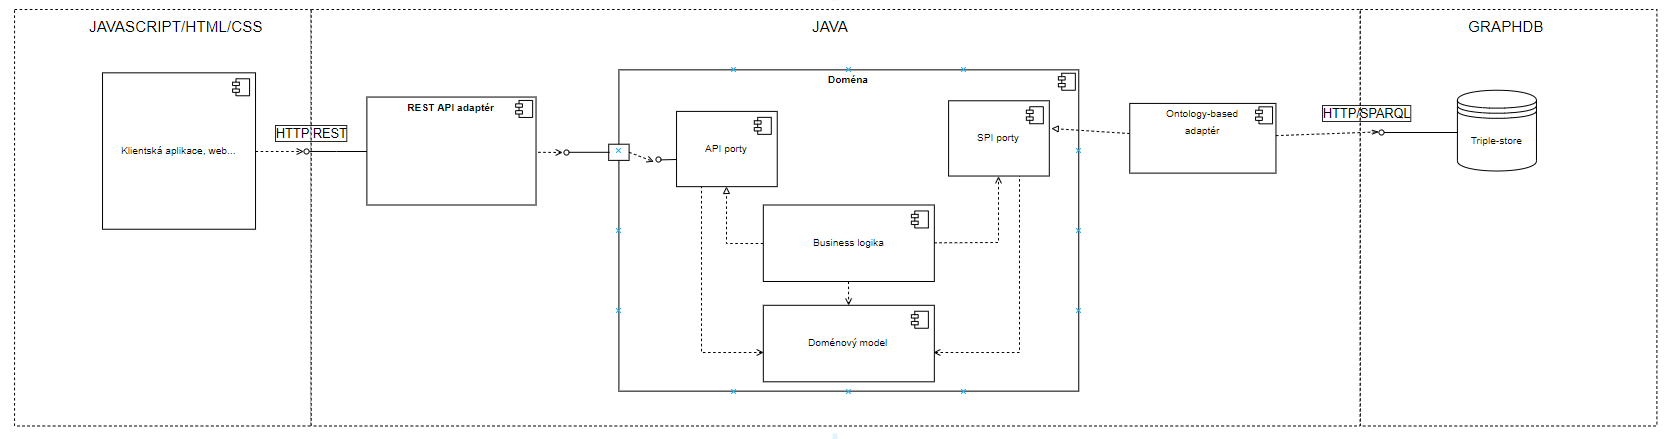
\includegraphics[width=\linewidth]{img/component-model-graphDB.png}
	\caption{Diagram komponent pro naše řešení (zdroj autor)}
	\label{fig:component-graphDB}
\end{sidewaysfigure}

\chapter{Ontologické schéma}
\begin{sidewaysfigure}[htbp!]
	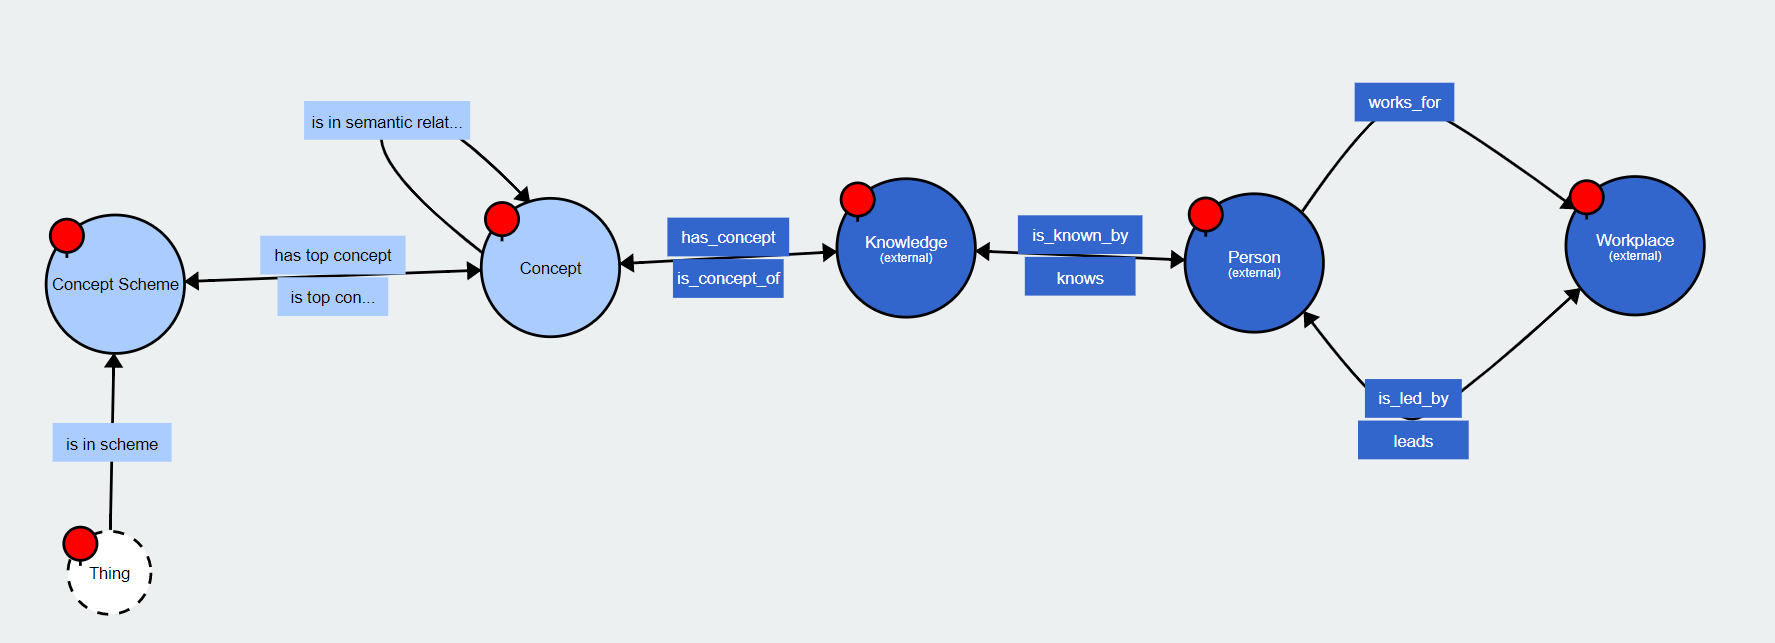
\includegraphics[width=\linewidth]{img/ontology-scheme.png}
	\caption{Použité ontologické schéma (zdroj autor, použitý nástroj \url{http://www.visualdataweb.de/webvowl/})}
	\label{fig:ontology-scheme}
\end{sidewaysfigure}

\chapter{SPARQL dotaz - vyhledávání osob dle kompetencí} \label{app:sparql-query}
\begin{lstlisting}[language=SPARQL, caption= SPARQL dotaz pro vyhledávání osob dle jejich kompetencí, captionpos=b]
    select ?person ?name ?surname ?username ?weight ?sub
    ?sub2 ?sub3 ?sub4 where {
         {
                ?person ?knows              ?k;
                        ?hasName            ?name;
                        ?hasUsername        ?username;
                        ?hasSurname         ?surname .
                ?k      ?hasWeight          ?weight;
                        ?hasConcept         ?concept .
        }
        UNION
        {
                ?person ?knows              ?k;
                        ?hasName            ?name;
                        ?hasUsername        ?username;
                        ?hasSurname         ?surname .
                ?k      ?hasWeight          ?weight;
                        ?hasConcept         ?sub1 .
                ?sub1   ?semanticRelation   ?concept .
        }
        UNION
        {
                ?person ?knows              ?k;
                        ?hasName            ?name;
                        ?hasUsername        ?username;
                        ?hasSurname         ?surname .
                ?k      ?hasWeight          ?weight;
                        ?hasConcept         ?sub1 .
                ?sub1   ?semanticRelation   ?sub2 .
                ?sub2   ?semanticRelation   ?concept .
        }
        UNION
        {
                ?person ?knows              ?k;
                        ?hasName            ?name;
                        ?hasUsername        ?username;
                        ?hasSurname         ?surname .
                ?k      ?hasWeight          ?weight;
                        ?hasConcept         ?sub1 .
                ?sub1   ?semanticRelation   ?sub2 .
                ?sub2   ?semanticRelation   ?sub3 .
                ?sub3   ?semanticRelation   ?concept .
        }  
        UNION
        {
                ?person ?knows              ?k;
                        ?hasName            ?name;
                        ?hasUsername        ?username;
                        ?hasSurname         ?surname .
                ?k      ?hasWeight          ?weight;
                        ?hasConcept         ?sub1 .
                ?sub1   ?semanticRelation   ?sub2 .
                ?sub2   ?semanticRelation   ?sub3 .
                ?sub3   ?semanticRelation   ?sub4 .
                ?sub4   ?semanticRelation   ?concept .
        }   
    }
\end{lstlisting}
\chapter{Výstup systému po vyhledání dle kompetencí} \label{app:search-result}
\begin{lstlisting}[language=JSON, caption= Výstup systému při dotazu na vyhledání dle kompetencí, captionpos=b]
   [
   {
      "person":{
         "name":"Tomáš",
         "surname":"Sobotka",
         "username":"sobotat",
         "id":"http://onto.fel.cvut.cz/koubadom/individuals/persons
         #Tomas_Sobotka"
      },
      "metric":0.5,
      "info":"Source: GraphDB Info: 0 intermediate concepts"
   },
   {
      "person":{
         "name":"Jiří",
         "surname":"Žák",
         "username":"zakji",
         "id":"http://onto.fel.cvut.cz/koubadom/individuals/
         persons#Jiri_Zak"
      },
      "metric":0.3,
      "info":"Source: GraphDB Info: 2 intermediate concepts"
   },
   {
      "person":{
         "name":"Michal",
         "surname":"Sáblík",
         "username":"sablimi",
         "id":"http://onto.fel.cvut.cz/koubadom/individuals/persons
         #Michal_Sablik"
      },
      "metric":0.2,
      "info":"Source: GraphDB Info: 3 intermediate concepts"
   },
   {
      "person":{
         "name":"Pavel",
         "surname":"Zapravda",
         "username":"zaprapa",
         "id":"http://onto.fel.cvut.cz/koubadom/individuals/persons
         #Pavel_Zapravda"
      },
      "metric":0.18,
      "info":"Source: GraphDB Info: 4 intermediate concepts"
   }
]
\end{lstlisting}


\chapter{Seznam použitých technologií, nástrojů a knihoven} \label{app:technology-list}
\paragraph{Serverová část:}
\begin{itemize}
    \item \textbf{Java 8} a její prostředí, SDK v1.8.0\_92 (\url{https://www.java.com/en/})
    \item \textbf{Spring Boot} a přidružené knihovny (\url{https://spring.io/projects/spring-boot})
    \item \textbf{JOPA} (\url{https://github.com/kbss-cvut/jopa})
    \item \textbf{Maven} (\url{https://maven.apache.org/})
    \item \textbf{GraphDB Free} (\url{http://graphdb.ontotext.com/})
\end{itemize}
\paragraph{Klientská část:}
\begin{itemize}
    \item \textbf{Javascript} (implementaci následujícího \url{https://www.ecma-international.org/ecma-262/5.1/} )
    \item \textbf{npm} (\url{https://www.npmjs.com/})
    \item \textbf{Webpack} a přidružené knhovny (\url{https://webpack.js.org/})
    \item \textbf{HTML5} (\url{https://www.w3.org/TR/html52/})
    \item \textbf{CSS3} (\url{https://www.w3.org/TR/css-2018/})
\end{itemize}
\paragraph{Nástroje:}
\begin{itemize}
    \item \textbf{IntelliJ IDEA} (\url{https://www.jetbrains.com/idea/})
    \item \textbf{Webstorm} (\url{https://www.jetbrains.com/webstorm/})
    \item \textbf{Enterprise architect} (studentská verze) (\url{https://sparxsystems.com/})
    \item \textbf{Draw.io} (\url{https://www.draw.io/})
    \item \textbf{Prohlížeč Mozilla Firefox} (\url{https://www.mozilla.org/en-US/})
    \item \textbf{Prohlížeč Google Chrome} (\url{https://www.google.com/chrome/})
    \item \textbf{Protégé} (\url{https://protege.stanford.edu/})
\end{itemize}
\paragraph{Inspirace:}
\begin{itemize}
    \item \textbf{Reporting tool} (\url{https://github.com/kbss-cvut/reporting-tool/})
    \item \textbf{Spring-hexagonal-example}\par (\url{https://github.com/gshaw-pivotal/spring-hexagonal-example})
\end{itemize}
% [TODO: možná dát do přílohy zápis ze schůzky s panem Klímou]

\chapter{Obsah přiloženého CD} \label{app:cd-content}
\begin{itemize}
    \item \ctulst(none)!prototype.zip! - zdrojové soubory prototypu aplikace
    \item \ctulst(none)!db-scheme.zip! - databázové schéma ve formátu turtle
    \item \ctulst(none)!test-dataset.zip! - testovací dataset ve formátu turtle
    \item \ctulst(none)!text-source.zip! - zdrojové soubory textu
    \item \ctulst(none)!thesis.pdf! - elektronická verze tohoto textu
\end{itemize}
	
\end{document}

